\documentclass{article}

\usepackage{staking}
\usepackage{listings}
\lstset{
  language=python,
  % xleftmargin=35pt,
  numbersep=10pt,
  tabsize=2,
  showspaces=false,
  showstringspaces=false,
  backgroundcolor=\color{backcolour},
  commentstyle=\color{codegreen},
  % keywordstyle=\color{codeblack} % \color{magenta},
  stringstyle=\color{codepurple},
  basicstyle=\sffamily\tiny,
  captionpos=b,
}

\usepackage[utf8]{inputenc} % allow utf-8 input
\usepackage[T1]{fontenc}    % use 8-bit T1 fonts
\usepackage{hyperref}       % hyperlinks
\usepackage{url}            % simple URL typesetting
\usepackage{booktabs}       % professional-quality tables
\usepackage{amsfonts}       % blackboard math symbols
\usepackage{nicefrac}       % compact symbols for 1/2, etc.
\usepackage{microtype}      % microtypography
\usepackage{lipsum}
\usepackage{fancyhdr}       % header
\usepackage{graphicx}       % graphics
\usepackage{float}
\usepackage{setspace}
\usepackage{array}
\usepackage[fleqn]{amsmath}
\usepackage{caption}
\captionsetup{
  margin=35pt, 
  font={scriptsize, onehalfspacing}, 
  labelfont=bf, 
  textfont=sf,
  format=plain, 
  % indention=1cm, 
  labelsep=period, 
  parskip=5pt, 
  skip=2pt
}

% \usepackage[style=numeric, sorting=ynt] {biblatex}
\usepackage[backend=biber, sorting=none]{biblatex}
% \addbibresource{refs.bib}
\addbibresource{references.bib}

% \usepackage{natbib}
% \bibliographystyle{plain}

\graphicspath{{media/}}     % organize your images and other figures under media/ folder

%Header
\pagestyle{fancy}
\thispagestyle{empty}
\rhead{ \textit{ }} 
  
%% Title
\title{Optimized Decentralized Reward Distribution(1)}

\author{
  Chun-Hu Cui\\
  \texttt{fleetpro@gmail.com} \\
   \And
  He-Song Cui\\
  \texttt{jsreputation@gmail.com} \\
}


\begin{document}

\onehalfspacing

\maketitle


\begin{abstract}
  In DeFi (Decentralized Finance) applications, and in dApps (Decentralized Application) 
  generally, it is common to periodically pay interest to users as an 
  incentive, or periodically collect a penalty from them as a deterrent. 
  If we view the penalty as a negative reward, both the interest and penalty problems 
  come down to the problem of 
  distributing rewards. Reward distribution is quite accomplishable in financial 
  management where general computers are used, 
  but on a blockchain, where computational resources are inherently expensive 
  and the amount of computation per transaction is absolutely limited with a predefined, 
  uniform quota, not only do the system administrators have to pay heavy gas fees 
  if they handle rewards of many users one by one, but the transaction may also be 
  terminated on the way. 
  The computational quota makes it impossible 
  to guarantee processing an unknown number of users.

  We propose novel algorithms that solve Simple Interest, Simple Burn, Compound Interest, 
  and Compound Burn tasks, which are typical components of DeFi applications. 
  If we put numerical errors aside, these algorithms realize accurate distribution of 
  rewards to an unknown number of users with no approximation, 
  while adhering to the computational quota per transaction.
    For those who might already be using similar algorithms, 
  we prove the algorithms rigorously so that they can be 
  transparently presented to users.
  We also introduce reusable concepts and notations in decentralized reasoning,
  and demonstrate how they can be efficiently used.
  We demonstrate, through simulated tests spanning over 128 simulated years, 
  that the numerical errors do not grow to a dangerous level.

\end{abstract}

% keywords can be removed
\keywords{DeFi \and dApp \and staking reward 
\and reward distribution \and pendency tracker \and activity tracker }

\section{Introduction}
Saving computational resources is a general demand in all computing applications, 
but it has become a vital need in blockchains.
Blockchains impose a unilateral, uniform, and unconditional quota on the amount of 
computation that can be used for a transaction. 
Administrators as well as users must adhere to the quota while also paying 
a significant amount of fees in proportion to the amount of computation consumed.
We cannot trade off the integrity, consistency, and transparency requirements 
of applications to work around the quota problem, because the fact that blockchain is 
selected as the platform in the first place means we cannot compromise on the requirements.

The problem of overcoming the high computational cost and the computational quota 
per transaction arises especially when processing arrays of unknown length.
Suppose, for example, there is a requirement to “pay each user 0.01 \% interest 
every day based on the amount they keep staked.” 
On a general computer platform, it is possible and common to enumerate all users, 
calculate their interest amount, and send the amount to their accounts. However, 
the computational quota per transaction on blockchains make it a necessity to find 
fundamentally different solutions.
An immediate naive solution is to restrict the number of users, which is unacceptable.

The next idea is to process a certain number of users in one transaction and repeat 
a similar transaction several times until covering all users. 
The flaw is that the repetition has to be initiated and controlled 
from the off-chain part by system administrators, or, equivalently, by 
their administration automation tools.
This will prevent the achievement of the integrity, consistency, and transparency goal 
that called for choosing blockchain as the platform in the first place. 
If administrators and off-chain administration tools 
were such reliable, they wouldn't have chosen the expensive blockchain as the platform 
in the first place.

Some algorithms implement reward distribution to an unknown number of users 
without enumerating users. The earliest one is the 
prize distribution algorithm adopted in the MasterChef smart contract of the PancakeSwap 
DeFi application.
Instead of calculating each and every user’s prize share each time a new total 
prize is collectively available to users, 
they maintain the accumulated prize dividend index for each unit 
of total share (so, of each users' share) each time before the total share 
(so a user's share) changes its value.
The prize per share is used by all other users to calculate their 
pending prize.
This allows administrators to pretend to have processed users’ prize without 
actually having processed them all.
This \textit{virtual} processing method has been a model for many applications. 
We also gain inspiration from this method.

We formulate our methodology in Section~\ref{sec:Methodology}.
We first identify reward distribution tasks that we handle in this paper, 
(see Section~\ref{sec:Tasks}),
in terms of firstly how much rewards should theoretically be available for the dApp 
to distribute to users, 
and secondly whether the rewards are added to the same account as their principal account 
or to a separate asset account.
Simple Interest, Simple Burn, Compound Interest, and Compound Burn are the types of 
reward distribution tasks that we identify and aim to find algorithms for in this paper.
See Table~\ref{tbl:PendencyAndActivity} for the task types and their algorithm names.

We then introduce the Consistency Criteria for a reward distribution algorithm, 
as well as Relative Errors as a derived concept.
See Section~\ref{sec:Criteria} for the Consistency Criteria and 
Relative Errors.
Relative Errors are then used to assess the accuracy and 
numerical errors of our algorithms.

We finally discuss several imaginary types of reward distribution tasks 
and identify the position of our aimed reward distribution tasks among 
those concepts. See Section~\ref{sec:Position} for more.

We present and prove our algorithms in Section~\ref{sec:Algorithms}.
We depict them in UML State Machine diagrams for quick 
reference and comprehension. 
We find two alternative algorithms for each 
aimed reward distribution task: pendency tracker and activity tracker. 
See Table~\ref{tbl:PendencyAndActivity} for the classification of algorithms.

\begin{table}[H]
  % \begin{center}
    \begin{spacing}{1.8}\centering
      \fontsize{8pt}{8pt}\selectfont
      \begin{tabular} {|m{3cm} |m{5cm} |}
      \hline
      {\textbf{Task type}} & {\textbf{Algorithms that do not handle errors}} \\
      \hline
      {\textbf{Simple Interest}} & 
      {Simple Interest Pendency tracker} \newline {Simple Interest Activity tracker} \\[3mm]
      \hline
      {\textbf{Simple Burn}} &
      {Simple Burn Pendency tracker} \newline {Simple Burn Activity tracker} \\[3mm]
      \hline
      {\textbf{Compound Interest}} &
      {Compound Interest Pendency tracker} \newline {Compound Interest Activity tracker} \\[3mm]
      \hline
      {\textbf{Compound Burn}} &
      {Compound Burn Pendency tracker} \newline {Compound Burn Activity tracker} \\[3mm]
      \hline
    \end{tabular}
    \end{spacing}
  % \end{center}
  \caption {Classification of algorithms}
  \label{tbl:PendencyAndActivity}
  \end{table}

The term $pendency$ and $activity$ are two alternative variables that 
represent the state of a reward distribution algorithm. 
They both allow tracking an aspect of reward distribution, but it turns 
out that they each have unique pros and cons.
The activity tracker algorithms are proved symbolically by mathematical 
induction. We demonstrate that appropriate concepts and notations 
can help reasoning of decentralized processes.

Section~\ref{sec:RandomAlgorithms} discusses numerical error 
sources of the algorithms. There are two types of numerical error sources 
theoretically. Errors coming from integer expression of the exponentiation 
of fractional numbers are exponentiation errors, 
while errors coming from integer expression of the division of integers 
are division errors. Both types of errors are small enough to ignore, if 
we don't have extensively many transactions in our applications, 
although we propose an idea of how to mitigate division errors.

Section~\ref{sec:Tests} discusses our simulation tests and their results on our 
four reward distribution task types.
Despite that the Relative Errors in some tasks increase linearly, or 
even exponentially, over block numbers, 
they are less than $10^{-11}$ in compound tasks and less than $10^{-22}$ 
in simple tasks in our particular simulated tests, which span 128 simulated 
years and assume quite steep interest/penalty rates and modest frequency 
of transactions.

\section{Methodology}
\label{sec:Methodology}

\subsection{Tasks}
\label{sec:Tasks}
Throughout this paper, we assume decentralized reward distribution applications  
where users' digital assets are stored on a \textit{smart contract}, 
and all changes to the assets are only made through and by access functions 
defined by the smart contract. Without losing generality, we assume 
\textit{solidity} language as our smart contract programming language.
\textit{Reward distribution} is defined, for the purpose of this paper, 
as \textit{making the assets that are theoretically available to users physically 
available to them by crediting the assets to or debiting the assets from their 
destination accounts,} 
or by getting ready to fulfill any compatible asset transfer requests immediately.

We identify types of reward distribution tasks below, in terms of both the 
\textit{amount} and textit{destination} of rewards. We only handle numerical 
amount of assets and don't care of the nature and usage of the assets, 
which is up to particular applications.
We note it is customary to burn up collected penalties and to call the 
penalty a burn in Decentralized Applications.
We follow the custom and may call the penalty simply a burn.
We also note that interest is a positive reward while burn is a negative reward.

For short notations, $U$ denotes the set of all possible users,
throughout this paper.

\begin{itemize}
  \item Simple Interest

  \begin{figure}[H]
    \centering
    % \fbox{\rule[-.5cm]{4cm}{4cm} \rule[-.5cm]{4cm}{0cm}}
    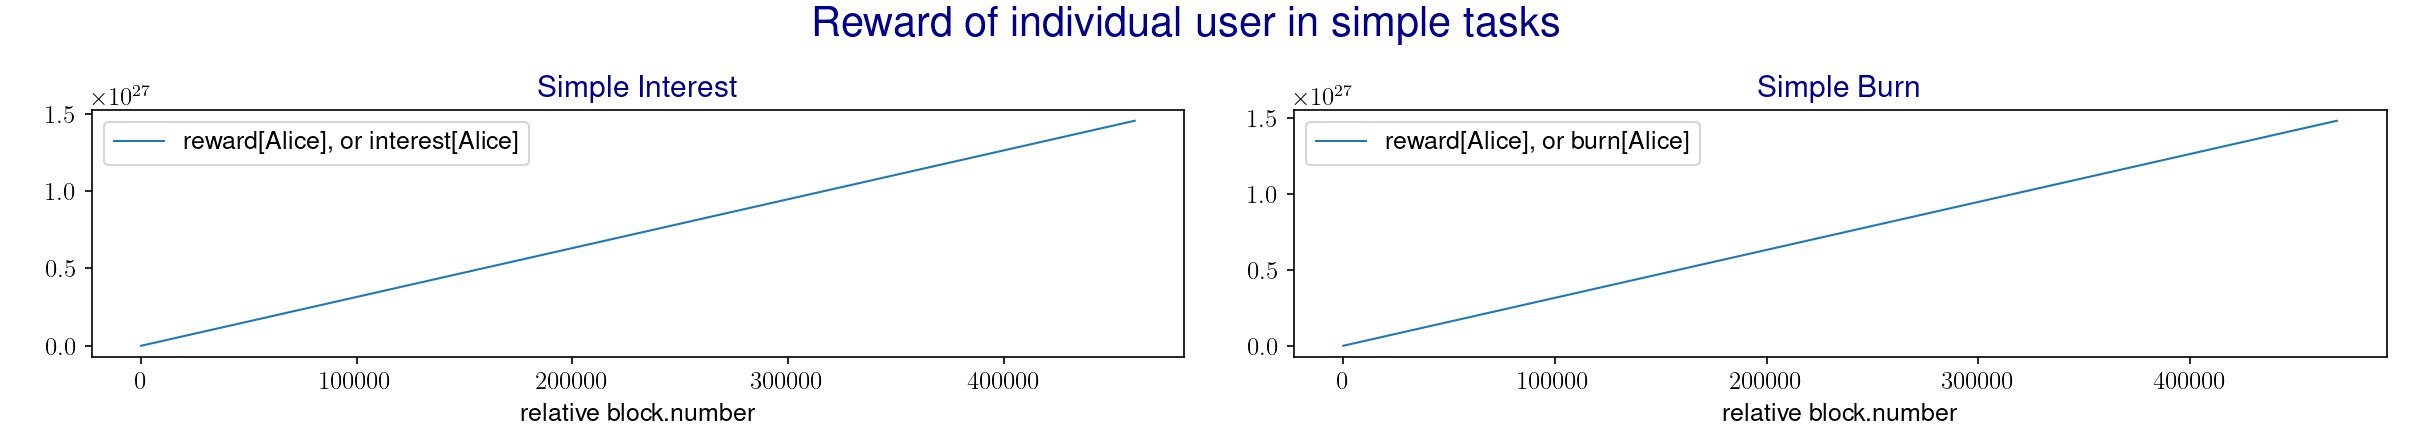
\includegraphics[width=5.3in]{images/_6.3_free_sim_individual_rewards.jpg}
    \caption{In a simple task, 
    $reward(user)$ for any user $user$, as well as $\sum_{u \in U}reward(u)$,
    grows linearly over time, because simple tasks only collect  
    rewards that grow linearly over time and the collected rewards 
    have their own account different from the principal account.
    }
    \label{fig:free_sim_individual_rewards}
  \end{figure} 

  \label{sec:SimpleInterest} 
  Simple Interest is a type of reward distribution task where the amount 
  and destination of rewards are defined by the following programming pseudocode:  
  \begin{equation} \label{eq:SimpleInterest}
    \\reward[user] = reward[user] + principals[user] *  rate  * blocks / cycle
    \end{equation}
    where $user$ is the user to whom the rewards are distributed, $reward[user]$ is the 
    reward destination account that stores $user$'s rewards, $principals[user]$ is 
    $user$'s amount of principal, $blocks$ is the number of blockchain 
    blocks that elapses, $cycle$ is a certain positive integer, 
    and $rate$ is the 
    interest rate formulated: "the interest as much as $rate$ portion of $principal$
    should be paid to the user every $cycle$ blocks that elapses." 
    The meaning and notation of variables 
    are the same throughout this paper, except that $rate$ refers to 
    the penalty rate in burn tasks and is formulated: 
    "the penalty as much as $rate$ portion of $principal$ should be collected from 
    the user every $cycle$ blocks that elapses."

    In this task, the user earns interest proportional to the interest rate and time 
    that elapses on their principal.
    The interest is accumulated to its own account separate from that of the principal, 
    and is \textit{not} credited to the principal account.
    The rewards can even be a different type of asset from the principal. 
    See Figure~\ref{fig:free_sim_individual_rewards} for more.
    We choose block number, rather than block timestamp, as the measure of 
    time for security reasons. The interest being simply additively accumulated in an account 
    does not define how the interest is processed or used in particular applications.

  \item Simple Burn
  \label{sec:SimpleBurn}

  Simple Burn is a type of reward distribution task where the amount 
  and destination of rewards are defined by the following programming pseudocode:
  \begin{equation}  \label{eq:SimpleBurn}
  \\reward[user] = reward[user] + principals[user] * rate * blocks / cycle
  \end{equation}
  In other words, the user is charged with a penalty proportional to the penalty rate 
  and time that elapses on their principal.
  The penalty has its own destination account different from that of principal, and 
  is \textit{not} debited from the principal amount.
  The penalty can even be a different type of asset from the principal. 
  See Figure~\ref{fig:free_sim_individual_rewards} for more.
  The penalties, which are negative rewards, are simply 
  positively accumulated in the reward account, because our algorithms do not 
  extend to taking care of how the penalty is exercised or materialized in particular 
  applications.
    
  \item Compound Interest

  \begin{figure}[H]
    \centering
    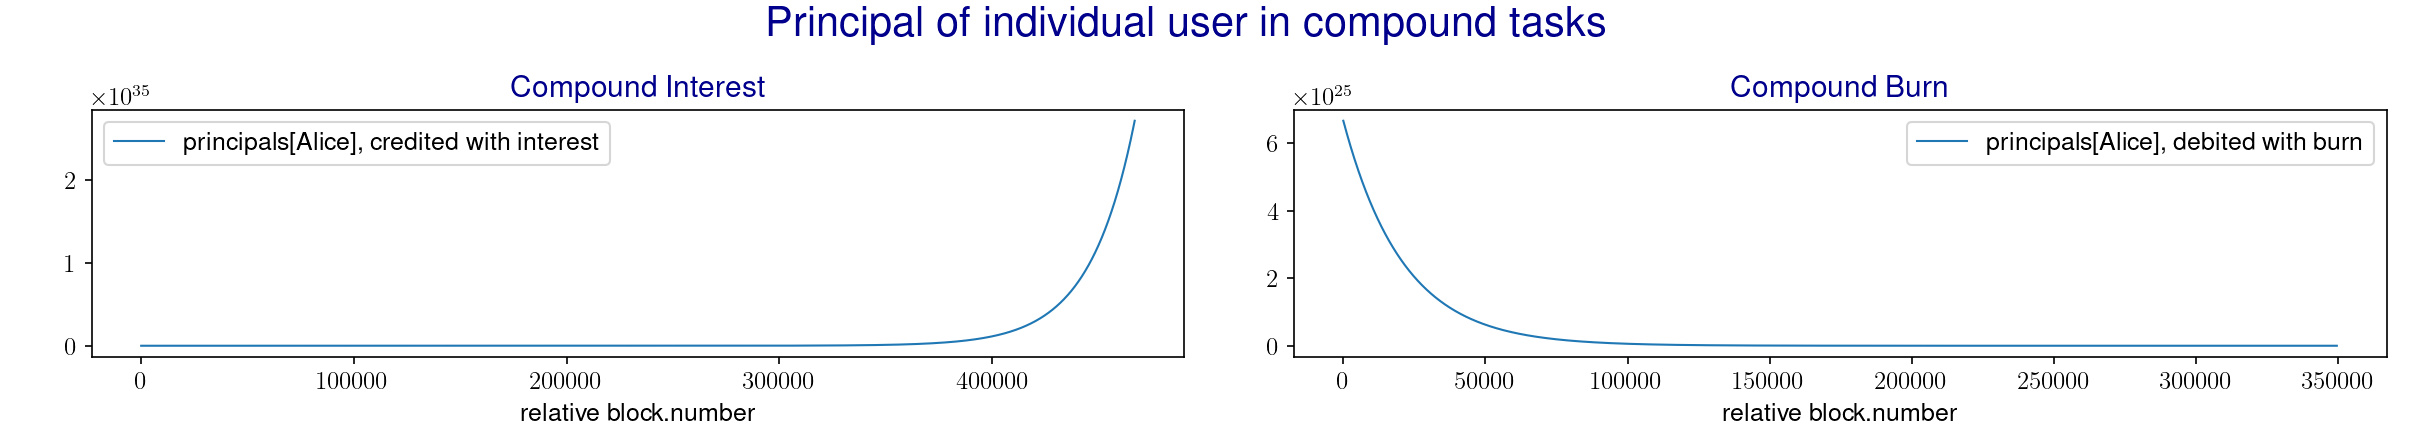
\includegraphics[width=5.3in]{images/_6.3_free_com_individual_principals.jpg}
    \caption{In a compound task,
    $balance(user)$ for any user $user$, which is $user$'s $principal$ plus/minus 
    $user$'s interest/burn, as well as $\sum_{u \in U}balance(u)$, 
    grows/shrinks exponentially from its initial value, because compound tasks 
    only collect interest/burn that is exponential over time and the collected 
    interest/burn is credited to/debited from the principal account.
    }
    \label{fig:free_com_individual_principals}
  \end{figure}

  \label{sec:CompoundInterest}
  Compound Interest is a type of reward distribution task where the amount 
  and destination of rewards are defined by the following programming pseudocode:
  \begin{equation}  \label{eq:CompoundInterest}
  \\principals[user] = principals[user] + principals[user] * ((1+rate)^{blocks/cycle}-1)
  \end{equation}
  In other words, interest is created by the amount $principal[user]$ and credited   
  to the $principal[user]$ account.
  Rigorously,
  the user continuously earns time-linear interest on their principal amount 
  while the earned interest is continuously credited to the principal amount. 
  The continuity is implemented by exponentiation.
  The interest and principal 
  not only share the same asset type with each other but also share the same account.
  See Figure~\ref{fig:free_com_individual_principals} for more.

  \item Compound Burn
  \label{sec:CompoundBurn}

  Compound Burn is a type of reward distribution task where the amount 
  and destination of rewards are defined by the following programming pseudocode:
  \begin{equation}  \label{eq:CompoundBurn}
  \\principals[user] = principals[user] - principals[user] * (1-(1-rate)^{blocks/cycle})
  \end{equation}
  In other words, the burn (penalty) is created by the amount $principal[user]$ and debited  
  from the $principal[user]$ account.
  Rigorously, 
  the user continuously pays a time-linear burn on their principal 
  while the paid burn is continuously debited from the principal amount. 
  The continuity is implemented by exponentiation.
  The penalty and principal 
  not only share the same asset type with each other but also share the same account.
  See Figure~\ref{fig:free_com_individual_principals} for more.

  \item Simple Shared Prize \newline
  \label{sec:SimpleSharedPrize}
  Simple Shared Prize is a type of reward distribution task where the amount 
  and destination of rewards are defined by the following programming pseudocode:
  \begin{equation}  \label{eq:SimpleSharedPrize}
    \\reward[user] = reward[user] + principals[user] / totalPrincipal *  alpha  * blocks / cycle,
  \end{equation}
  where $alpha$ is a constant that determines the total prize created for all users 
  collectively over time.
  The user earns their share of the total prize 
  $alpha  * blocks / cycle$. The earned rewards have a separate account 
  from that of the principal.
\end{itemize}

Simple tasks are simple because the rewards are destined to a separate account and they 
may even be of different asset type, 
whereas compound tasks are compound because the rewards are destined to the principal account, 
either by adding to or subtracting from the existing principal. 

We propose algorithms that solve the former \textit{four} tasks, under the 
conditions that the number of users is unknown and there is a computational 
quota. The 5th task is used as a reference to understand the former four tasks.

\subsection{Position}
\label{sec:Position}

We discuss the position of our aimed task types identified in Section~\ref{sec:Tasks} 
on the map of possible 
reward distribution policies. \newline
We can identify several imaginable types of reward distribution task types that can be 
thought of but unreasonable practically, in order to clarify the position of our aimed types 
of reward distribution tasks, as follows:

\begin{itemize}
  \item Simple Interest Exponential \newline
  \label{sec:SimpleInterestExponential}
  Simple Interest Exponential is an \textit{unreasonable} type of reward distribution task 
  where the amount and destination of rewards are defined by the following programming 
  pseudocode:
  \begin{equation} \label{eq:SimpleInterestExponential}
    \\reward[user] = reward[user] + principals[user] * ((1+rate)^{blocks/cycle}-1)
  \end{equation}
  The more frequently rewards are collected according to this formula, 
  the less total reward the user will earn. Users will not move, unless.
  If this formula is intentionally used to discourage them from collecting their rewards frequently, 
  the algorithm is likely found by tweaking our algorithms.
  
  \item Simple Burn Exponential \newline
  \label{sec:SimpleBurnExponential}
  Simple Burn Exponential is an \textit{unreasonable} type of reward distribution task 
  where the amount and destination of rewards are defined by the following programming 
  pseudocode:  
  \begin{equation} \label{eq:SimpleBurnExponential}
    \\penalty[user] = penalty[user] + principals[user] * ((1-rate)^{blocks/cycle}-1)
  \end{equation}
  The more frequently penalty is paid according to this formula, 
  the less total penalty the user will pay. Users will not rest, unless. 
  If this formula is intentionally used to encourage them to pay penalty frequently, 
  the algorithm is likely found by tweaking our algorithms.
  
  \item Compound Interest Linear \newline
  \label{sec:CompoundleInterestLinear}
  Compound Interest Linear is an \textit{unreasonable} type of reward distribution task 
  where the amount and destination of rewards are defined by the following programming 
  pseudocode:
  \begin{equation} \label{eq:CompoundleInterestLinear}
    \\principals[user] = principals[user] + principals[user] * (alpha * rate * blocks/cycle)
  \end{equation}
  The more frequently the reward is collected according to this formula, 
  the more total reward the user will earn. Users will not rest, unless.
  The algorithm, nonetheless, is likely found by tweaking our algorithms.
  
  \item Compound Burn Linear \newline
  \label{sec:CompoundBurnLinear}
  Compound Burn Linear is an \textit{unreasonable} type of reward distribution task 
  where the amount and destination of rewards are defined by the following programming 
  pseudocode:  
  \begin{equation} \label{eq:SimpCompoundBurnLinearleInterest}
    \\principals[user] = principals[user] - principals[user] * (alpha * rate * blocks/cycle)
  \end{equation}
  The more frequently the penalty is paid according to this formula, 
  the less total penalty the user will pay. Users will not rest, unless.
  The algorithm is likely found by tweaking our algorithms.
\end{itemize}

We exclude Simple Shared Prize type of tasks from our goal, because 
\begin{itemize}
  \item The algorithm created by the Pancakeswap dApp can correctly answer 
  $pending(user)$ for Simple Shared Prize tasks.
  (See Equation~\ref{eq:SimpleSharedPrize} for the formula of Simple Shared Prize.)
  \item We can extend with ease the PancakeSwap algorithm to correctly answer $balance(user)$, 
  $totalPending()$, and $totalBalance()$ for any Simple Shared Prize tasks, 
  by using a similar logic as used for other task types in this paper.
  See Section~\ref{sec:Criteria} for $balance(user)$, $totalPending()$, 
  and $totalBalance()$.
\end{itemize}

Our \textit{goal} is, therefore, to find algorithms that distribute rewards 
that are generated continuously over time to users for Simple Interest, Simple Burn, 
Compound Interest, and Compound Burn tasks, for an unknown number of users and 
adhering to the computational quota.

To the best of our knowledge, virtual distribution was invented by the PancakeSwap 
DeFi application.
Their virtual distribution method is often used as a model to work around the computational 
quota in subsequent Decentralized Applications.
We confirm, however, that our goal can \textit{not} be accomplished by tweaking the 
PancakeSwap’s algorithm.
In their algorithm, a user's rewards are generated by 
the \textit{relative} amount of the user's principal, while on our tasks, 
a user's rewards are generated by the \textit{absolute} amount of the user's principal. 
See Section~\ref{sec:Tasks} for their respective reward formulas.
There have been frequent attempts to solve the Compound Interest and Compound Burn 
tasks, raising several concepts, for example, around Compound Interest: 
periodic compound, manual compound, continuous compound, and automatic compound.
We should make it clear \textit{which} of the concepts relate \textit{how} to our algorithms.
We discuss these concepts one by one, although they are \textit{not} exclusive of 
each other.

To avoid confusion, compounding itself refers to adding interest to the principal that 
created the interest or subtracting a burn (penalty) from the principal that caused 
the burn.
The amount of interest to be compounded can be either 
$principal * ((1+rate)^{period}-1)$ or $principal * rate * period$, which we call 
the time-exponential interest and the time-linear interest, respectively. 
As with burn tasks, they are 
$principal * ((1-(1-rate)^{period}))$ and $principal * rate * period$,
and called time-exponential burn and time-linear burn, respectively.

\begin{itemize}
  \item Periodic Compound

  This task literally compounds periodically, either regularly or irregularly. 
  The compounding must be a part of a blockchain 
  transaction and the transaction must be invoked either by administrators or 
  users. 
  Periodic compounding of time-linear interest by users' transactions 
  may cause a meaningless competition or bank-run between users, because 
  the more frequently they compound, the more interest they earn.
  \textit{Periodic compounding by users is reasonable for time-exponential 
  interest}, as frequency has no effect on compounding time-exponential interest.
  Periodic compounding of time-linear interest by administrators' transactions,
  on the other hand,  
  might hurt users if administrators or administration automation tools fail 
  to call compounding in time, restricting the growth of users' interest.
  Periodic compounding of time-exponential interest by administrators' transactions 
  might cause users to await, if they fail, for the next round of compounding to 
  be unleashed. Administrators don't need to \textit{unreasonably} take compounding 
  over while users can \textit{reasonably} take responsibility for that.
  
  \item Manual Compound

  If manual compounding means compounding with direct personal involvement 
  of people rather than by off-chain automation tools, then we need to note 
  that people are the most unreliable component in a Decentralized Application, 
  unless the people are users compounding for themselves. 
  Users compounding for themselves means users in need of their compounding 
  call compounding at their discretion. \textit{This will allow them to be 
  responsible for their rewards}. 
  If manual compounding means compounding by administrators' transactions,
  rather than by users', and if administrators fail, then compounding may stop 
  while users are still using the system.
  
  \item Automatic Compound

  If automatic compounding means compounding with no direct personal involvement of 
  people but with their automation tools, off-chain tools are second most unreliable 
  component for a Decentralized Applications, unless the tools are operated by users 
  for themselves and at their discretion. 
  If automatic compounding means compounding with no direct involvement of 
  administrators, then it is with the involvement of users and by users' transactions.
  \textit{Compounding will not stop as long as users in need of compounding keep using 
  the system}, if compounding is left to users.
  
  \item Continuous Compound

  We cannot compound continuously, as nobody wants to invoke compounding transactions 
  every block.
  Continuous compounding can be viewed as 
  periodic compounding of time-linear interest with an infinitely small compounding period. 
  This does not necessarily mean calling compounding transactions in every block, 
  which too is not enough to be continuous.
  \textit{Continuous compounding can be implemented by, periodically or intermittently, 
  regularly or irregularly, compounding time-exponential interest.} 
  As mentioned above, frequency has no effect on compounding time-exponential interest. 
  \textit{Continuous compounding, or compounding time-exponential 
  interest, is only reasonable if invoked by users for themselves.}

\end{itemize}

We observe above that the desirable compounding should be by users' transactions 
compounding time-exponential interest for users themselves at their discretion, 
whether it be manual or automatic. (Manual and automatic are not defined clearly.)
A Decentralized Application, after all, should be in operation only while there are 
users using it, not while there are administrators.
Users will, immediately or eventually, have to pay more for more gas, 
but gas fees cannot warrant compounding called by administrators.

We follow this observation and 
\textit{choose, regular or irregular, compounding of time-exponential interest carried out  
by users' transactions for users themselves, whether it be manual or automatic.}

Carrying out compounding by users' transactions leads to getting compounding actions,
which are part of our algorithms, \textit{parasitic on users' transactions}.
Technically, this is implemented by our algorithms hooking user transactions, 
working inside the transactions' context, and collecting pending rewards before the transactors 
perform their intended actions, 
although true dynamic hooking is not possible on a blockchain and in Solidity language.
\textit{Coincidentally, normal users' transactions work better if pending rewards have 
been collected before performing their intended actions}. 
For example, when a user transfers a portion of their net principal to someone else, 
the user wants to collect pending interest into the principal account before transferring.
Generally, compounding actions should get parasitic on \textit{every} principal-changing 
transaction and precede it. Any user transactions that require compounding 
to precede themselves may want compounding actions to get \textit{parasitic} on themselves.
The transactions include: mint, burn, transfer, stake, un-stake, harvest, etc.
See List~\ref{lst:parasitic} for how to implement compounding actions parasitic on 
users' transactions.
\newline

\label{lst:parasitic}
\begin{lstlisting} [
  % float,
  caption={Example of $changePrincipal(user, amount)$ function parasitic on transactions. 
  The $changePrincipal(user)$ function in our algorithms acts as the compounding action 
  that gets parasitic on users' transactions and precedes the transactions' intended actions. 
  This function collects all pending rewards of the user and adds it to their destination account.
  \textit{Furthermore}, the function
  takes over principal-chaining actions from the transactions, as 
  compounding actions and principal-changing actions have high 
  cohesion and should be in the same module, from the software engineering 
  point of view.  }
]
  function mint(user, amount) {
    changePrincipal(user, amount); # Collect user's pending rewards, and credit user's principal
  }
  function transfer(sender, recipient, amount) {
    changePrincipal(sender, -amount); # Collect sender's pending rewards, and debit their principal
    changePrincipal(recipient, amount); # Collect recipient's pending rewards, and credit their principal
  }
\end{lstlisting}

One of the \textit{thumb rules} that we learn from the previous  
and this section is that reasonable simple tasks handle linear rewards 
whereas reasonable compound tasks handle exponential rewards.

\subsection{Consistency criteria}
\label{sec:Criteria}

We clarify the following terms:

\begin{itemize}
  \item If \textit{a distribution is made actually}, all users' entitled 
  rewards are moved to their respective destination accounts.
  \item If \textit{a distribution is made actually and immediately}, 
  the distribution is made actually, as soon as users are entitled to 
  some rewards.
\end{itemize}

Algorithms that distribute rewards to an unknown number of users should act 
\textit{as if all distributions were made actually and immediately}, 
while actual distributions are deferred until suitable moments of time, 
because immediate actual distribution to all users is not guaranteed to 
succeed due to the computational quota and possibly excessively large number of users.
Acting this way is called \textit{making virtual reward distribution}. 

For a query into a reward distribution process, 
we clarify the term \textit{return value} and \textit{true value}:
\begin{itemize}
  \item return value, for a query, is the value returned by an algorithm 
  that is running in a particular program, in response to the query.
  \item true value, for a query, is the value that exists for the query
  purely by accounting principals and independently of algorithms and programs.
\end{itemize}

A reward distribution algorithm that is running in a particular program 
is said to be \textit{consistent} at a moment  
if and only if the \textbf{\textit{Consistency Criteria}}, 
defined below, are satisfied at the moment:

\begin{itemize}
  \item A query $pending(user)$'s return value $pending(user)$ equals 
  its \textit{true value} $\{pending(user)\}$ for any user $user$,
  which is the current amount of reward that $user$ is entitled to 
  but is not yet actually distributed.

  \item A query $balance(user)$'s return value $balance(user)$ equals 
  its \textit{true value} $\{balance(user)\}$ for any user $user$,
  which is the balance of $user$'s reward destination account 
  plus/minus $pending(user)$. (Minus is for burn tasks.)
  Equivalently, it answers to "what would the balance of $user$'s 
  reward account be if all distributions were made actually and immediately."
  We note that in compound tasks the reward account is the same as the principal 
  account, unlike in simple tasks. 
  See Section~\ref{sec:Tasks} for more about task types.
  
  \item A query $totalPending()$'s return value $totalPending()$ equals 
  its \textit{true value} $\{totalPending()\}$,
  which is $\sum_{u \in U} \{pending(user)\}$.
  This query has its own significance, as it may be impossible to sum up across all users.
  Algorithms find this value indirectly.

  \item A query $totalBalance()$'s return value $totalBalance()$ equals 
  its \textit{true value}, $\{totalBalance()\}$,
  which is $\sum_{u \in U}\{balance(user)\}$.
  This query has also its own significance, as it may be impossible to sum up across 
  all users. Algorithms find this value indirectly.

  \item The algorithm allows consistent transfers,
  meaning that the algorithm allows all transfers of any amount of asset  
  from the reward destination account of any user $user$ if the amount is equal to or 
  less than $balance(user)$, unless the application prohibits the transfers.

\end{itemize}

The Consistency Criteria can be simplified as:
\begin{itemize}
  \item $pending(user) = \{pending(user)\}$ for any user $user$
  \item $balance(user) = \{balance(user)\}$ for any user $user$
  \item $totalPending() = \{totalPending()\}$
  \item $totalBalance() = \{totalBalance()\}$
  \item the algorithm allows consistent transfers
\end{itemize}

Algorithms may not be consistent, because they may 
\begin{itemize}
  \item have errors in their logic, unlike our algorithms
  \item have an approximation in their logic, unlike our algorithms
  \item suffer numerical errors of computer operation, \textit{like} 
  our algorithms
\end{itemize}

We prove that our algorithms have no errors in their logic by rigorously 
verifying that \textit{our algorithms are consistent} at any moment, 
in the next section.

As for numerical errors, we discuss the errors theoretically and in 
simulated tests.
We introduce the following \textit{Consistency Errors} as performance measures 
of our algorithms running in a particular program:

  \begin{equation} \label{eq:TrueTotal}
    TrueTotal = \{totalBalance()\} = \sum_{u \in U} \{balance(user)\}
  \end{equation}

  \begin{equation}  \label{eq:AbsoluteErrorA}
    Absolute \hspace{3pt} Error \hspace{3pt} A = |totalBalance() - TrueTotal|
  \end{equation}

  \begin{equation}  \label{eq:AbsoluteErrorB}
    Absolute \hspace{3pt} Error \hspace{3pt} B = |\sum_{u \in U} balance(u) - TrueTotal|
  \end{equation}

  \begin{equation}  \label{eq:RelativeErrorA}
    Relative \hspace{3pt} Error \hspace{3pt} A = |totalBalance() - TrueTotal| / TrueTotal
  \end{equation}

  \begin{equation}  \label{eq:RelativeErrorB}
    Relative \hspace{3pt} Error \hspace{3pt} B = |\sum_{u \in U} balance(u) - TrueTotal| / TrueTotal
  \end{equation}

  Consistency Errors only takes care of $balance(user)$, and not of $pending(user)$, 
  because $balance(user)$ is not independent of $pending(user)$ but is an accumulation of 
  $pending(user)$. Absolute Error and Relative Error may be called Absolute Consistency Error 
  and Relative Consistency Error, respectively.

\section{Algorithms}
\label{sec:Algorithms}

In this section, the eight algorithms for our four task types are proved 
to be consistent at any moment, under the assumption that there are no 
computer numerical errors, as is not the case.
See Table~\ref{tbl:PendencyAndActivity} 
for a classification of the eight algorithms.
Numerical errors are handled in the last 
subsection \ref{sec:RandomAlgorithms}, where random 
algorithms that mitigate some of numerical errors are proposed and discussed.

The algorithms presented below are in the form of UML 
State Machine diagram, without losing rigorosity. 
We choose verbal proof for pendency tracker algorithms,
and choose symbolic proof for activity tracker algorithms, for comparison.

\subsection{Simple Interest pendency tracker algorithm}
\label{sec:SimpleInterestPendency}

\begin{figure}[H]
  \centering
  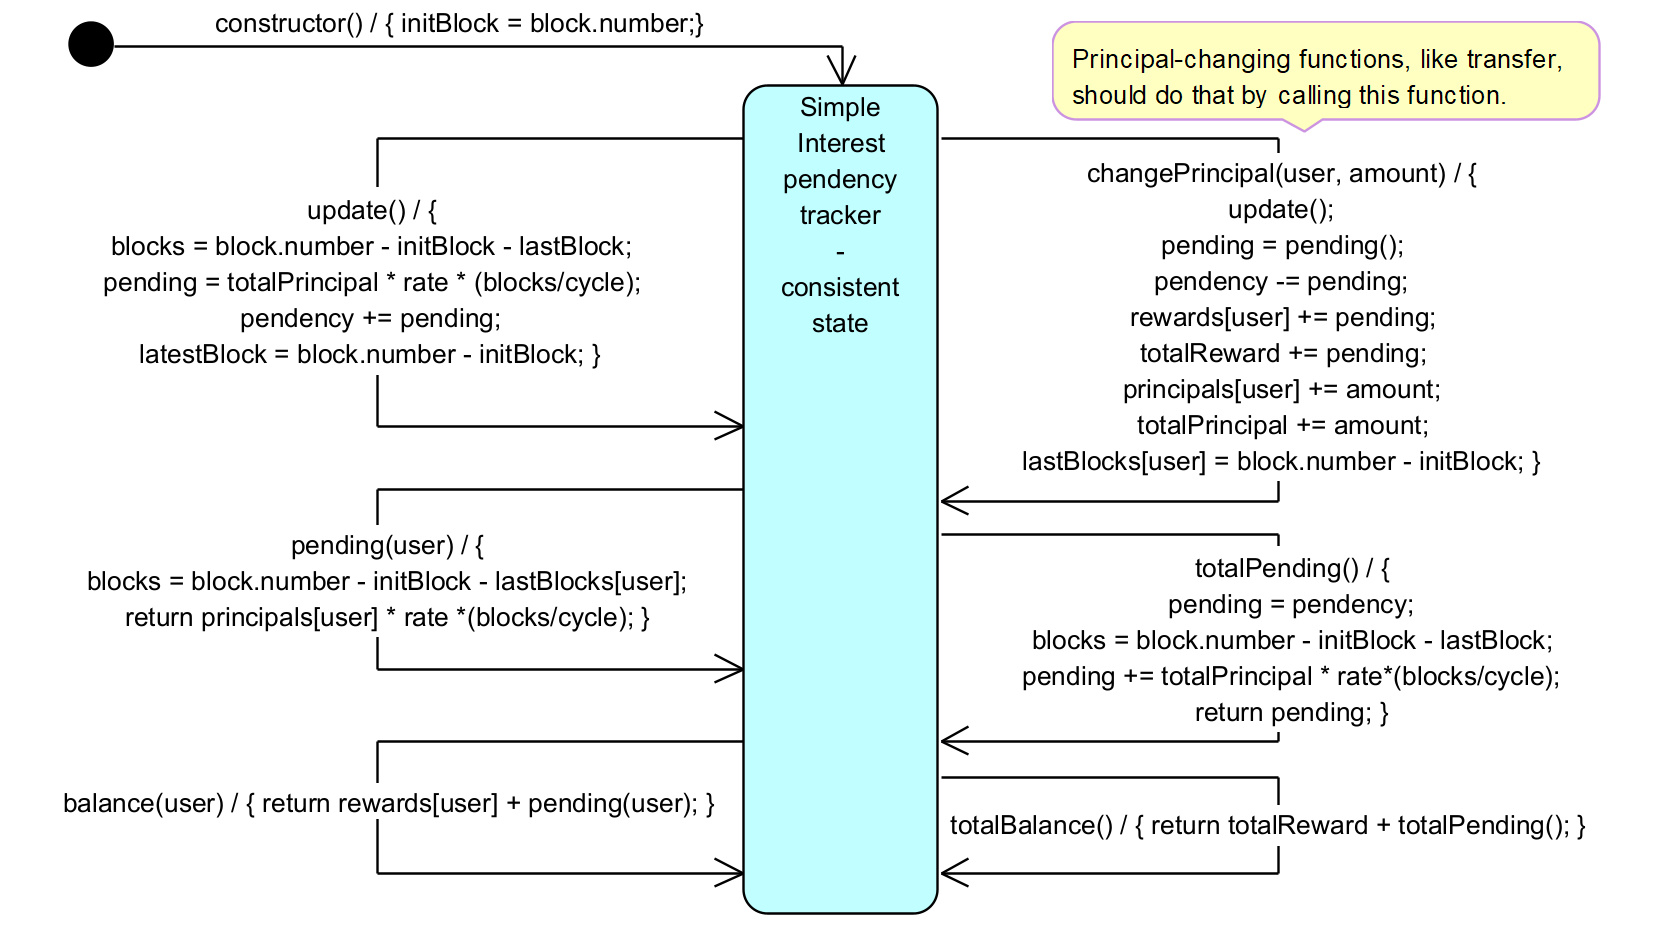
\includegraphics[width=5.3in]{images/SimpleInterestPendency.jpg}
  \caption{The UML State Machine of Simple Interest pendency tracker algorithm. 
  The four functions corresponding to queries in the Consistency Criteria,  
  as well as the $changePrincipal(user,amount)$ function, are represented  
  as events of the state machine.
  When invoked, these events are supposed to let the state machine transition 
  from the \textit{consistent state} back to the same \textit{consistent state}.
  }
  \label{fig:SimpleInterestPendency}
\end{figure}
See Equation~\ref{eq:SimpleInterest} for the formula of Simple Interest tasks.
See Figure~\ref{fig:SimpleInterestPendency} for the state machine of the algorithm.

The algorithm can be proved as follows:

The $changePrincipal(user, amount)$ function collects and compounds all pending
interest of a given user $user$, 
whenever \textit{before} changing the variable $principals[user]$, 
because the interest formula Equation~\ref{eq:SimpleInterest} is a function 
of a \textit{constant} $principals[user]$ 
and the elapsed time period over which the $principals[user]$ 
remained that constant.
After finishing the $changePrincipal(user, amount)$ function, 
the $user$'s pending interest becomes zero. 
This justifies the logic of the 
$pending(user)$ function, which simply returns the rewards created after the 
latest call on the $changePrincipal(user, amount)$ function.

As for the $totalPending()$ function, the variable $pendency$ is tracked by 
the $update()$ and $changePrincipal(user, amount)$ functions for the user 
$user$ who is currently calling a principal-changing transaction, which, in 
turn, calls the current instance of $changePrincipal(user, amount)$ 
function.
The variable $pendency$ is added, in the $update()$ function, 
with the \textit{total interest} newly created 
by the existing total principal $totalPrincipal$ during the period over which 
the total Principal was kept to the current constant, whenever before the total 
principal is changed, so, whenever before a user's principal is changed.
That newly created total interest should represents \textit{all} users' newly 
created interest for the same period.
The variable $pendency$ is then subtracted with \textit{the} user's pending 
interest and the user's reward account is credited with that pending interest, 
effectively distributing the user's pending interest to the user, via $pendency$.
Therefore, the variable $pendency$ indicates the total pending 
interest, as of the latest $changePrincipal(user, amount)$ call, that is not yet 
actually distributed to individual users other than \textit{the} very user.
When asking the $totalPending()$ query, the additional interest created 
after the latest $changePrincipal(user, amount)$ call is returned together with 
the $pendency$.

The $balance(user)$ function is straightforward. The balance of a user is 
the sum of their rewards, which is collected and accumulated interest of the 
user, and their pending interest. The $totalBalance()$ is similar.

This algorithm is called a pendency tracker, because the $totalPending()$ 
function is calculated by using a representation of pending amount, $pendency$.

\subsection{Simple Burn pendency tracker algorithm}
\label{sec:SimpleBurnPendency}

\begin{figure}[H]
  \centering
  % \fbox{\rule[-.5cm]{4cm}{4cm} \rule[-.5cm]{4cm}{0cm}}
  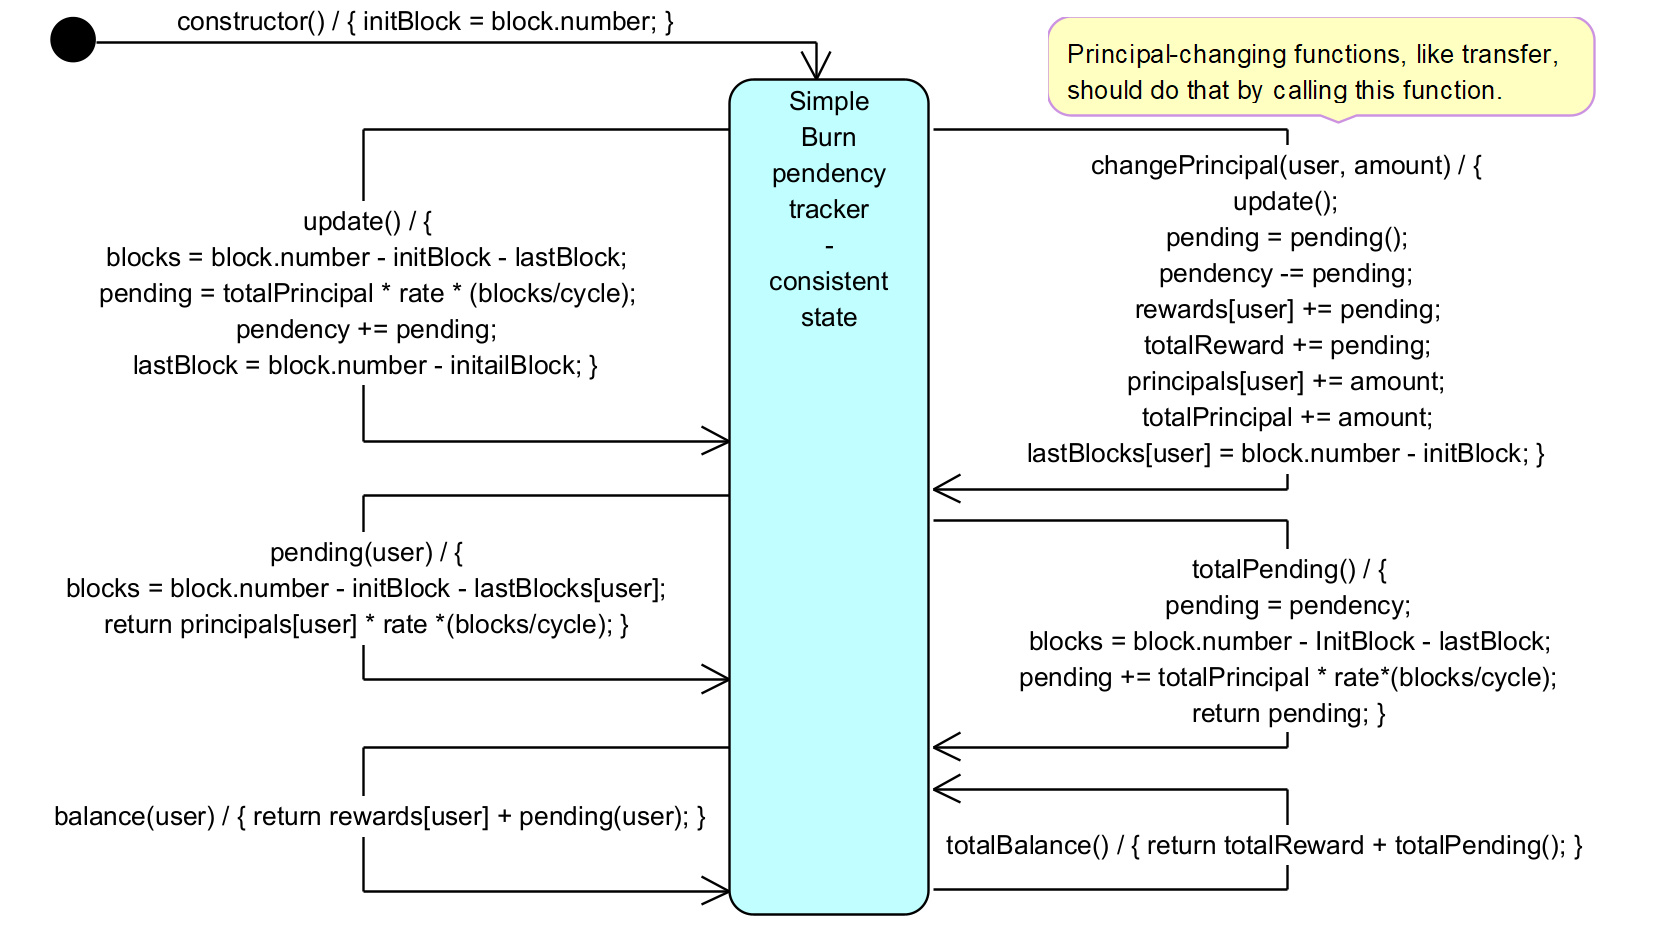
\includegraphics[width=5.3in]{images/SimpleBurnPendency.jpg}
  \caption{The UML State Machine of Simple Burn pendency tracker algorithm.
  }
  \label{fig:SimpleBurnPendency}
\end{figure}
See Equation~\ref{eq:SimpleBurn} for the formula of Simple Burn tasks.
See Figure~\ref{fig:SimpleBurnPendency} for the state machine of the 
algorithm.
\newline
We note in the functions $balance(user)$ and $totalBalance()$, the pending penalty,
which is the penalty theoretically charged but not yet actually distributed, 
is added to, and not subtracted from, the user's reward. 
This is because these algorithms solve only quantitative relationships and do 
not relate to how the assets are materialized, simply accumulating charged penalties 
into the negative reward account.

This algorithm can be proved similarly as in Simple Interest Pendency tracker.

\subsection{Compound Interest pendency tracker algorithm}
\label{sec:CompoundInterestPendency}

\begin{figure}[H]
  \centering
  % \fbox{\rule[-.5cm]{4cm}{4cm} \rule[-.5cm]{4cm}{0cm}}
  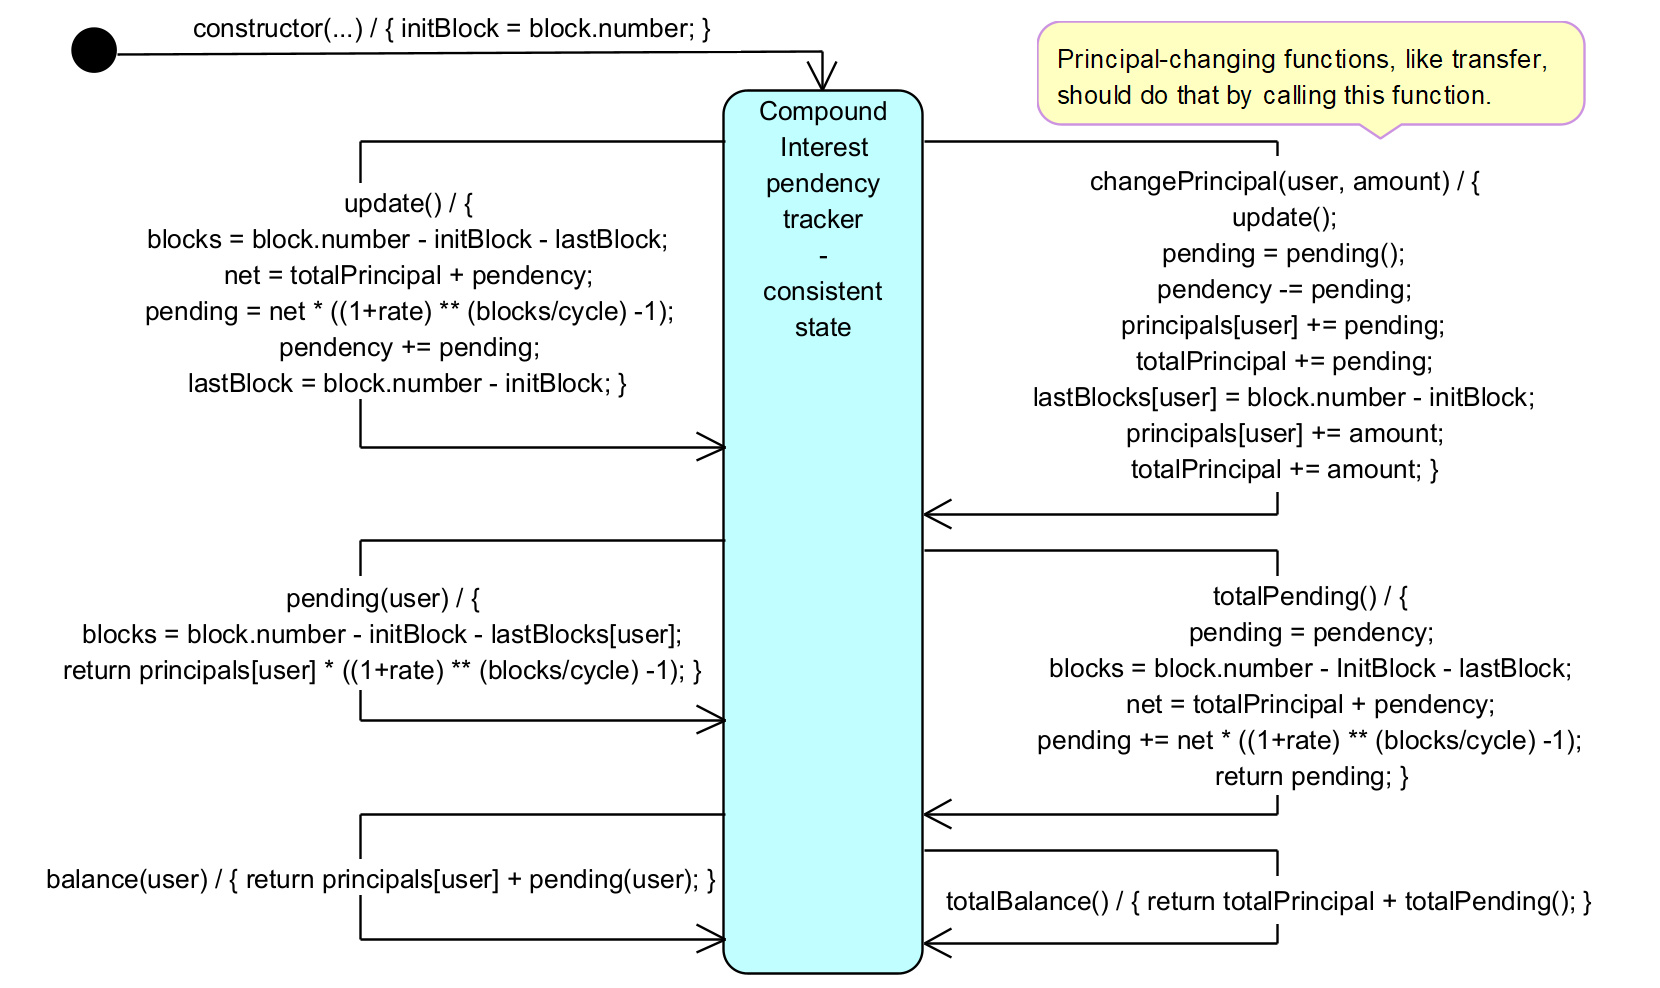
\includegraphics[width=5.3in]{images/CompoundInterestPendency.jpg}
  \caption{The UML State Machine of Compound Interest pendency tracker algorithm.
  }
  \label{fig:CompoundInterestPendency}
\end{figure}
See Equation~\ref{eq:CompoundInterest} for the formula of Compound Interest tasks.
See Figure~\ref{fig:CompoundInterestPendency} for the state machine of the 
algorithm.
% \newpage

\subsection{Compound Burn pendency tracker algorithm}
\label{sec:CompoundBurnPendency}

\begin{figure}[H]
  \centering
  % \fbox{\rule[-.5cm]{4cm}{4cm} \rule[-.5cm]{4cm}{0cm}}
  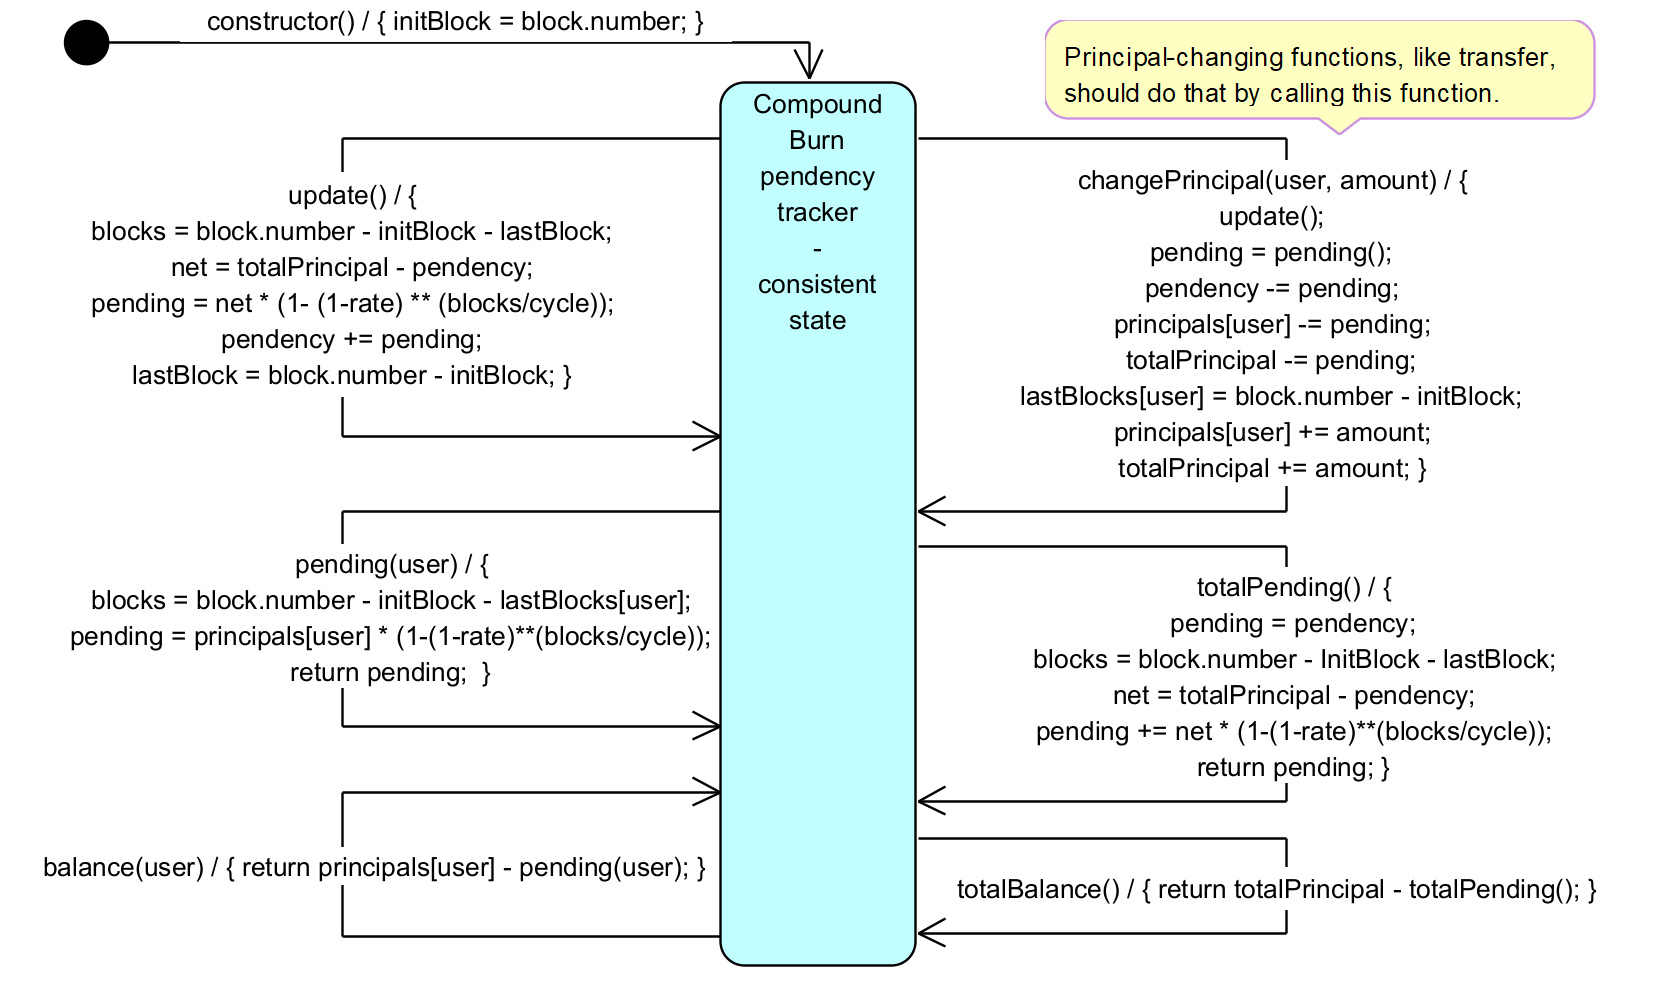
\includegraphics[width=5.3in]{images/CompoundBurnPendency.jpg}
  \caption{The UML State Machine of Compound Burn pendency tracker algorithm.}
  \label{fig:CompoundBurnPendency}
\end{figure}
See Equation~\ref{eq:CompoundBurn} for the formula of Compound Burn tasks.
See Figure~\ref{fig:CompoundBurnPendency} for the state machine of the Compound 
Burn pendency tracker algorithm.

This algorithm can be proved Similarly as in Simple Interest Pendency tracker

\subsection{Simple Interest activity tracker algorithm}
\label{sec:SimpleInterestActivity}

\begin{figure}[H]
  \centering
  % \fbox{\rule[-.5cm]{4cm}{4cm} \rule[-.5cm]{4cm}{0cm}}
  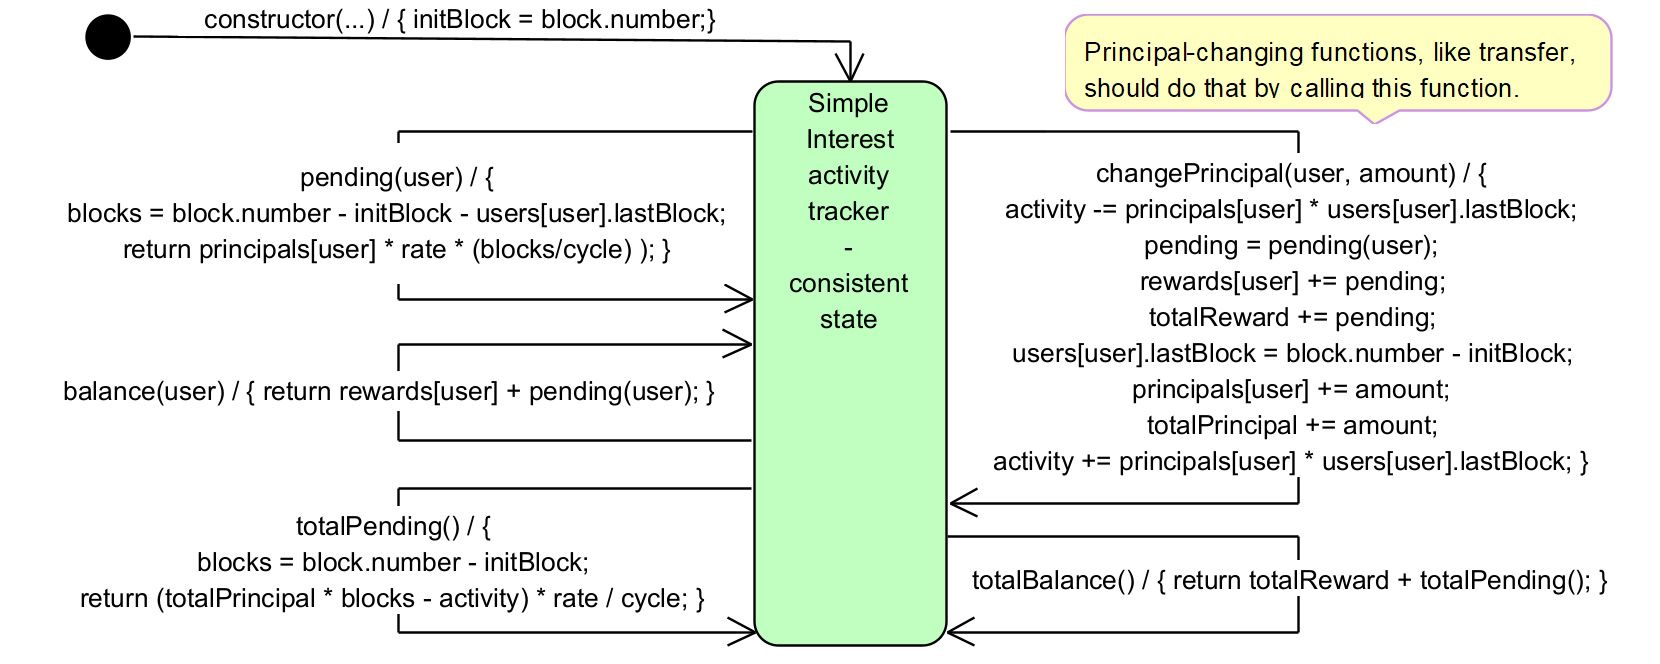
\includegraphics[width=5.3in]{images/SimpleInterestActivity.jpg}
  \caption{The UML State Machine of Simple Interest activity tracker algorithm.}
  \label{fig:SimpleInterestActivity}
\end{figure}

See Equation~\ref{eq:SimpleInterest} for the formula of Simple Interest tasks.
See Figure~\ref{fig:SimpleInterestActivity} for the state machine of the Simple  
Interest \textit{activity} tracker algorithm. 

\label{sec:Pendency_vs_Activity}
Unlike \textit{pendency} tracker algorithms 
presented so far that track the amount of rewards that are not yet distributed,
\textit{activity} tracker algorithms track a representation of
users' activity in terms of how long time users keep how much principal.
Symmetric, they should be equivalent, but it is observed that the two performs 
not the same and not necessarily one is better than the other in all aspects.
Pendency tracker and activity tracker algorithms are alternatives to each other 
and we can choose between them in practice according to specific task requirements.
See Section~\ref{sec:Tests} for more.

We introduce the following definitions and notations, which might be used in  
symbolic reasoning of general blockchain techniques:

\begin{itemize}
  \item {\textbf{History}} is a set of identified events in a particular 
  decentralized application program.
  \begin{itemize}
    \item The identified events primarily may include all transactions in the program.
    \item If the task has a transaction in a block, then the block can also be included in the 
    identified events.
    \item The initial block \textbf{$initBlock$}, where the decentralized 
    application program is deployed on the blockchain, is included, in particular.
    \item We assume there is an event \textbf{$init$} where all variables are initialized 
    from no value to zero at the beginning of $initBlock$.
    \item If we need to identify the evaluation of a block of individual programming 
    statements in a particular transaction, 
    then the evaluation of those statements are also an event in the event history.
    \item Different programs may have different history for the same application class, 
    as each program relates to events of its own interest.
  \end{itemize} 
  \item {\textbf{Left moment of event e}, denoted by $e-$}, is the very start of the event $e$
  and has no duration. \textbf{Right moment of event e}, $e+$, is the very end of event $e$.
  For example, if $e$ is a block, then $e-$ is the start of the block;
  if $e$ is a transaction, then $e+$ is the end of the transaction; etc. 
  We assume $init-$ is equal to $initBlock-$, in particular.
  \item {\textbf{Moments of history $H$}, $M(H)$}, means $ \cup_{e \in H} \{ e-, e+\} $
  \item {\textbf{Ordered moments of history $H$}, $OM(H)$}, is a sequence 
  that consists of elements of the moments of history $H$ and that is arranged 
  in the order of taking place. The ordered moments of history exist uniquely 
  for a given history, and is 
  a finite-length sequence or has the same structure as natural numbers.
  \item {\textbf{Block of moment m}, $B(m)$} for a moment $m$, 
  is the block or block number where the moment takes place.
  \item {\textbf{Quantity Q as of moment m}}, $Q^{[m]}$ for a moment $m$, is the quantity of 
  property $Q$ that exists at the moment $m$.
  \item {\textbf{All users}, $U$}, is the set of all possible account addresses.
\end{itemize}

We also have the following definitions and notations specifically for this paper:

\begin{itemize}
  \item \textbf{Last block of user u at moment m}, 
  $u.lastBlock^{[m]}$, is the block or block number where the user 
  $u$'s principal changed latest before the given moment $m$.
  \item {\textbf{Principal of user u}, $principals[u]$}, is the amount of the principal 
  of user $u$.
  \item {\textbf{Interest/burn rate}, $rate$}, is an interest rate or burn rate 
  in the reward distribution application.
  \item {\textbf{Virtual rewarding period}, $cycle$}, is a certain positive integer 
  such that the interest/burn rate is described as "an interest/burn as much 
  as $rate$ portion of the principal is credited from/debited to its destination 
  account every $cycle$ block(s) that elapses." This is called a virtual because 
  we don't actually collect rewards every $cycle$ blocks.
\end{itemize}

The following abbreviations are used interchangeably 
for the remaining part of this paper:

\begin{itemize}
  \item $P$ for $principals$
  \item $lB$ for $lastBlock$
  \item $C$ for $cycle$
  \item $R$ for $rate$
\end{itemize}

We introduce the following definitions: 

\label{sec:AlgorithmCorrectness}
\begin{itemize}
  \item A reward distribution algorithm is said to be consistent for 
  a principal-changing 
  event $e$ if and only if the algorithm is consistent for any moment $m$ 
  over the moment interval $[e+, en-]$ where $en$ is the next coming 
  Principal-changing event.
  (See Section~\ref{sec:Criteria} for Consistency Criteria.)
  \item A reward distribution algorithm is said to be consistent if and only if 
  the algorithm is consistent for any principal-changing event $e$.
\end{itemize}

We prove that the Simple Interest activity tracker algorithm is consistent, 
by mathematical induction for principal-changing events, as follows:

\begin{itemize}
  \item \textbf{The algorithm is consistent for the initial principal-changing 
  event $init$}.  

  We have to prove that the algorithm is consistent at any moment $m$ over 
  the moment interval $[init+, n-]$ where $n$ is the next coming principal-chaining 
  event.
  Firstly, all the four queries in the Consistency Criteria   
  return zero; which is its true value, because the principals of all users  
  remain zero over the interval $[init+, n-]$, as there were no 
  principal-changing actions at all after all principals were initialized 
  to zero by the event $init$.

  Secondly, the algorithm allows consistent transfers, because $balance(user)$ is a 
  zero for any user $user$, and the algorithm can always transfer/debit a zero amount 
  from the reward destination account of $user$.

  \item \textbf{If we assume that the algorithm is consistent for a principal-changing 
  event $e$, then it is also consistent for the next coming principal-changing event $ne$ }.

  See Section~\ref{sec:Criteria} for Consistency Criteria. 
  Let $\dot u$ be the user whose principal is changed by the event $ne$, 
  then this proposition is proved as follows.

  \begin{itemize}

    \item[$\square$] $pending(u)^{[(u.lastBlock^{[e+]})+]} = 0$ for any user $u$.
    \newline \newline
    % Because for the moment $r = (u.lastBlock^{[e+]})+$,
    % \begin{align*}
    %   &pending(u)^{[r]} \\
    %   &= principals[u]^{[r]} * rate * (B(r) - u.lastBlock^{[r]}) \\
    %   &= P[u]^{[r]} * R * (B((u.lB^{[e+]})+) - u.lB^{[(u.lB^{[e+]})+]}) \\
    %   &= P[u]^{[r]} * R * (u.lB^{[e+]} - u.lB^{[e+]}) \\
    %   &= 0
    % \end{align*}
    Because, $pending(u)^{[r]}$, where $r = (u.lastBlock^{[e+]})+$,
    \newline \newline 
    $ = principals[u]^{[r]} * rate * (B(r) - u.lastBlock^{[r]}) $, by the algorithm
    \newline \newline 
    $ = P[u]^{[r]} * R * (B((u.lB^{[e+]})+) - u.lB^{[(u.lB^{[e+]})+]}) $
    \newline \newline 
    $ = P[u]^{[r]} * R * (u.lB^{[e+]} - u.lB^{[e+]}) $
    \newline \newline 
    $ = 0 $
    \newline

    \item[$\square$] $ activity^{[e+]} = \sum_{u \in U} principals[u]^{[e+]} * u.lastBlock^{[e+]}$.\\
    (See the algorithm state machine in Figure~\ref{fig:SimpleInterestActivity} for $activity$.)
    \newline \newline
    Because, {$ totalPending^{[e+]} $}
    \newline \newline
    $ = \sum_{u \in U} pending(u)^{[e+]} $, because the algorithm is consistent at $e+$,
    \newline \newline
    $ = \sum_{u \in U} \{ pending(u)^{[(u.lB^{[e+]})+]}
    + P[u]^{[(u.lB^{[e+]})+]} * R * (B(e+) - u.lB^{[e+]}) / C \}$
    \newline \newline
    $ = \sum_{u \in U} \{ P[u]^{[e+]} * R * (B(e+) - u.lB^{[e+]}) / C \}$,
    \newline \newline
   because
   \begin{itemize}
      \item[$\circ$] $pending(u)^{[(u.lB^{[e+]})+]} = 0$ for any user $u$; \newline

      \item[$\circ$] if $(B(e+) - u.lB^{[e+]}) = 0$ and, so, $P[u]^{[(u.lB^{[e+]})+]}$ 
      does not yet exist at the moment $e+$, then we can replace the multiplier 
      $P[u]^{[(u.lB^{[e+]})+]}$ with any value; \newline

      \item[$\circ$] if $(B(e+) - u.lB^{[e+]}) > 0$, then the user's principal didn't change 
      since its latest change and 
      \newline \newline
      $P[u]^{[(u.lB^{[e+]})+]} = P[u]^{[e+]}$. \newline
    \end{itemize}

    $ = ( \sum_{u \in U} P[u]^{[e+]} ) * B(e+) * R / C 
    - ( \sum_{u \in U} P[u]^{[e+]} * u.lB^{[e+]} ) * R / C $
    \newline \newline
    $ = (totalPrincipal^{[e+]} * B(e+) - ( \sum_{u \in U} P[u]^{[e+]} * u.lB^{[e+]} )) * R / C $
    \newline \newline
    On the other hand, the algorithm returns the following value to be $ totalPending^{[e+]} $:
    \newline \newline
    $ ( totalPrincipal^{[e+]} * B(e+) - activity^{[e+]} ) * rate / cycle $.
    \newline \newline
    Therefore, $ activity^{[e+]} = \sum_{u \in U} P[u]^{[e+]} * u.lB^{[e+]}$.
    \newline

    \item[$\square$] $ activity^{[ne+]} = \sum_{u \in U} principals[u]^{[ne+]} * u.lastBlock^{[ne+]}$.
    \newline \newline
    Because, $ activity^{[ne+]}$
    \newline \newline
    $ = activity^{[ne-]} - principals[\dot u]^{[ne-]} * \dot{u}.lastBlock^{[ne-]} + principals[\dot u]^{[ne+]} * u.lastBlock^{[ne+]} $
    \newline \newline
    $ = activity^{[e+]} - P[\dot u]^{[e+]} * \dot{u}.lB^{[e+]} + P[\dot u]^{[ne+]} * u.lB^{[ne+]} $
    \newline \newline
    $ = \sum_{u \in U} P[u]^{[e+]} * u.lB^{[e+]} - P[\dot u]^{[e+]} * \dot{u}.lB^{[e+]}
    + P[\dot u]^{[ne+]} * u.lB^{[ne+]} $ 
    \newline \newline
    $ = \sum_{u \in U \setminus \{\dot u\}} P[u]^{[e+]} * u.lB^{[e+]} + P[\dot u]^{[ne+]} * u.lB^{[ne+]} $
    \newline \newline
    $ = \sum_{u \in U \setminus \{\dot u\}} P[u]^{[ne+]} * u.lB^{[ne+]} + P[\dot u]^{[ne+]} * u.lB^{[ne+]} $
    \newline \newline
    $ = \sum_{u \in U} P[u]^{[ne+]} * u.lB^{[ne+]}  $
    \newline \newline
    Below, we assume any moment $r$ over the moment interval $[en+, o-]$ where $o$ is the next 
    coming principal-changing event after $en$, and prove that the algorithm is 
    consistent at the moment $r$.

    \item[$\square$] { $ pending(u)^{[r]}$ returns its true value for any user $u$.}
    \newline \newline
    Because, $ pending(u)^{[r]}$
    \newline \newline
    $ = principals[u]^{[r]} * rate * (B(r)-u.lastBlock^{[r]}) $
    \newline \newline
    $ = P[u]^{[e+]} * R * (B(r)-u.lB^{[r]}) $, for $u \neq \dot u$
    \newline \newline
    $ = P[u]^{[e+]} * R * (B(e+)-u.lB^{[e+]}+B(r)-B(e+))$, for $u \neq \dot u$
    \newline \newline
    $ = pending(u)^{[e+]} + P[u]^{[e+]} * R * (B(r)-B(e+))$, for $u \neq \dot u$
    \newline \newline
    where, from the assumption of induction, $pending(u)^{[e+]}$ returns 
    its true value; 
    and $P[u]^{[e+]} * R * (B(r_)-B(m+))$ is the true reward created 
    after the moment $e+$. Therefore, 
    $ pending(u)^{[r]}$ returns its true value for $u \neq \dot u$.
    \newline \newline
    For the user $\dot u$,
    \newline \newline
    $ principals[\dot u]^{[r]} * rate * (B(r)-u.lastBlock^{[r]}) $
    \newline \newline
    $ = P[\dot u]^{[ne+]} * R (B(r)-B(ne+)) $
    \newline \newline
    $ = pending(\dot u)^{[e+]} - pending(\dot u)^{[e+]} + P[\dot u]^{[ne+]} * R (B(r)-B(ne+)) $
    \newline \newline
    $ = pending(\dot u)^{[e+]} - pending(\dot u)^{[ne-]} + P[\dot u]^{[ne+]} * R (B(r)-B(ne+)) $
    \newline \newline
    where $pending(\dot u)^{[e+]}$ returns its true value, from the assumption of induction;
    $- pending(\dot u)^{[ne-]} $ has occurred by the $changePrincipal(u, amount)$ 
    function collecting the pending reward of the user $\dot u$ at the event $ne$;
    and $principals[\dot u]^{[ne+]} * R (B(r)-B(ne+))$ is 
    the true reward created after the moment $ne+$.
    Therefore, we can say $ pending(\dot u)^{[r]}$ returns its true value.

    \item[$\square$] { $ totalPending^{[r]} $ returns its true value.}
    \newline \newline
    Because, $totalPending^{[r]}$
    \newline \newline
    $ = (totalPrincipal^{[r]} * B(r) - activity^{[r]}) * rate / cycle $
    \newline \newline
    $ = totalPrincipal^{[ne+]} * B(r) * R / C - activity^{[ne+]} * R / C $
    \newline \newline
    $ = ((\sum_{u \in U} P[u]^{[ne+]} * B(r)) - (\sum_{u \in U} P[u]^{[ne+]} * u.lB^{[ne+]})) * R / C$
    \newline \newline
    $ = \sum_{u \in U} P[u]^{[u.lB^{[r]}+]} * (B(r)-u.lB^{[r]}) * R / C $
    \newline \newline
    $ = \sum_{u \in U} pending(u){[r]} $,
    \newline \newline
    where $pending(u){[r]}$ returns its true value for all users $u$.
    Therefore $ totalPending^{[r]} $ also returns its true value.
    
    \item[$\square$] { $ balance(u)^{[r]}$ returns its true value for any user $u$.} \newline
    Because, according to the algorithm, $balance(u)^{[r]} = reward[u]^{[r]} + pending(u)^{[r]}$,
    where $reward[u]^{[r]}$ is its true value 
    because it has been accumulated with historic true values $\{pending(u)\}$; 
    and $pending(u)^{[r]}$ is also proved above to be its true value.

    \item[$\square$] { $ totalBalance^{[r]} $ returns its true value.} \newline
    Because, according to the algorithm, $totalBalance^{[r]} = totalReward^{[r]} + totalPending^{[r]}$,
    where $totalReward^{[r]}$ is its true value 
    because it has been accumulated with historic true values $pending(user)$;
    and $totalPending^{[r]}$ is proved above to be its true value.

    \item[$\square$] The algorithm allows consistent transfers. \newline
    Because the algorithm collects and adds $pending(user)$ to the user's actual balance 
    so that the actual balance becomes the same amount as $balance(user)$ returns, 
    before calling the requested transfer actions, which can now transfer/debit 
    up to $balance(user)$ amount of asset from the actual balance.
  \end{itemize}

\end{itemize}

Thus far, the Simple Interest pendency tracker algorithm is proved to be consistent, 
in the meaning defined in Section~\ref{sec:AlgorithmCorrectness}.

\subsection{Simple Burn activity tracker algorithm}
\label{sec:SimpleBurnActivity}

\begin{figure}[H]
  \centering
  % \fbox{\rule[-.5cm]{4cm}{4cm} \rule[-.5cm]{4cm}{0cm}}
  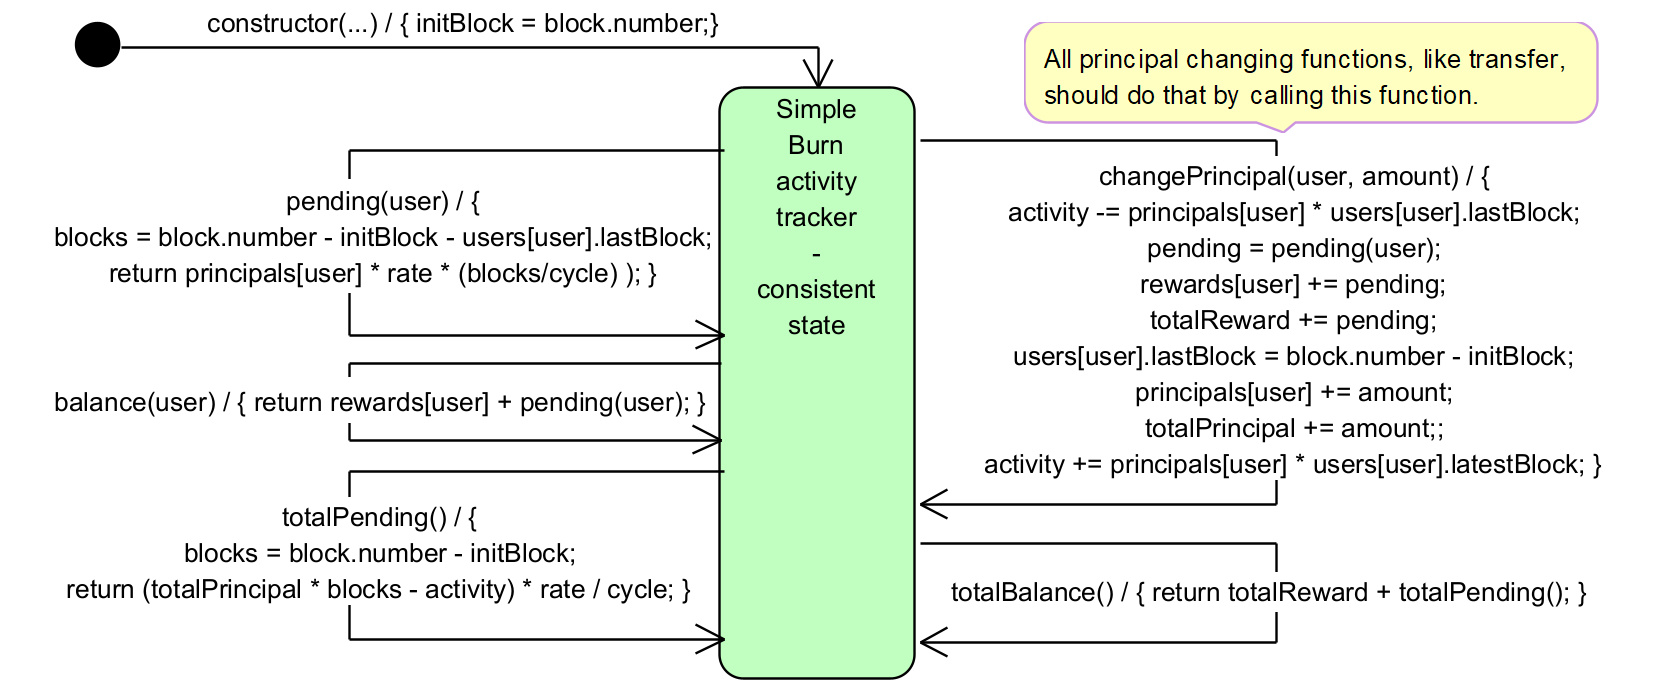
\includegraphics[width=5.3in]{images/SimpleBurnActivity.jpg}
  \caption{The UML State Machine of Simple Burn activity tracker algorithm.}
  \label{fig:SimpleBurnActivity}
\end{figure}
See Equation~\ref{eq:SimpleBurn} for the formula of Simple Burn tasks.

Figure~\ref{fig:SimpleBurnActivity} shows the state machine of the Simple  
Burn \textit{activity} tracker algorithm.

This algorithm has symbolically the same state machine diagram and 
the same proof as the Simple Interest activity tracker algorithm.

% \newpage

\subsection{Compound Interest activity tracker algorithm}
\label{sec:CompoundInterestActivity}

\begin{figure}[H]
  \centering
  % \fbox{\rule[-.5cm]{4cm}{4cm} \rule[-.5cm]{4cm}{0cm}}
  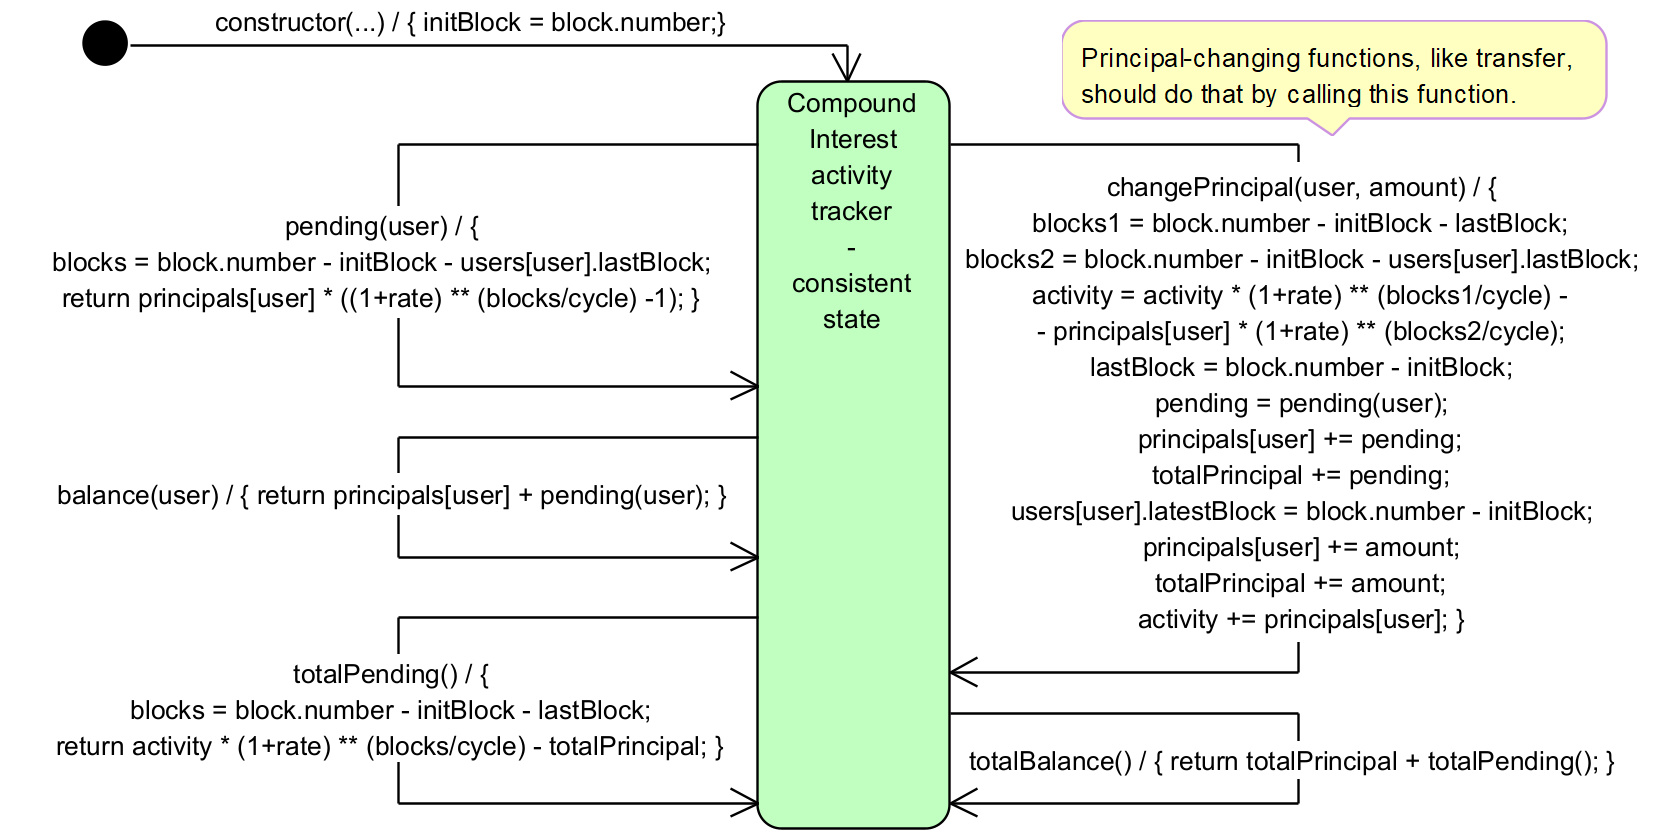
\includegraphics[width=5.3in]{images/CompoundInterestActivity.jpg}
  \caption{The UML State Machine of Compound Interest activity tracker algorithm.}
  \label{fig:CompoundInterestActivity}
\end{figure}
See Equation~\ref{eq:CompoundInterest} for the formula of Compound Interest tasks.

Figure~\ref{fig:CompoundInterestActivity} shows the state machine of the 
Compound Interest \textit{activity} tracker algorithm.

With the same definitions, notations, and assumptions as in Simple Interest 
activity tracker depicted in Figure~\ref{fig:SimpleInterestActivity},
we can prove the main part of the algorithm by mathematical induction for 
principal-chaining moments, as follows:

\begin{itemize}
  \item \textbf{The algorithm is consistent for the initial principal-changing 
  event $init$}.

  (See Section~\ref{sec:Criteria} for Consistency Criteria.)
  We have to prove that the algorithm is consistent for any moment $m$ over 
  the moment interval $[init+, n-]$ where $n$ is the next coming principal-chaining 
  event.
  Firstly, all the four queries in the Consistency Criteria 
  return zero; which is its true value, because the principals of all users  
  remained zero over the interval $[init+, m]$, as there were no 
  principal-changing actions after all principals were initialized 
  to zero at the moment $init+$.

  Secondly, the algorithm allows consistent transfers, because $balance(user)$ is 
  zero and the algorithm can always transfer/debit a zero amount 
  from the asset balance of the user $user$. 

  \item \textbf{If we assume that the algorithm is consistent for a principal-changing 
  event $e$, then it is also consistent for the next coming principal-changing event $ne$ }.

  (See Section~\ref{sec:Criteria} for Consistency Criteria.) 
  If $\dot u$ denotes the user whose principal is changed by the event $ne$, 
  this proposition is proved as follows:\\

  \begin{itemize}

    \item[$\square$] $pending(u)^{[(u.lastBlock^{[e+]})+]} = 0$, for any u $u$.
    \newline \newline
    Because, $pending(u)^{[r]}$, where $r = (u.lastBlock^{[e+]})+$,
    \newline \newline
    $ = principals[u]^{[r]} * ((1+rate)^{(B(r) - u.lastBlock^{[r]})}-1) $, by the algorithm,
    \newline \newline 
    $ P[u]^{[r]} * ((1+R)^{(B((u.lB^{[e+]})+) - u.lB^{[(u.lB^{[e+]})+]})}-1) $
    \newline \newline 
    $ P[u]^{[r]} * ((1+R)^{0}-1) $
    \newline \newline 
    $ = 0 $
    \newline
    \item[$\square$] $ activity^{[e+]} = \sum_{u \in U} principals[u]^{[e+]} * (1+rate )^{(B(e+)-u.lastBlock^{[e+]})/cycle}$.
    \newline
    (See the algorithm state machine in Figure~\ref{fig:CompoundInterestActivity} for $activity$.)
    \newline \newline
    Because, {$ P^{[e+]} $}
    \newline \newline
    $ = \sum_{u \in U} pending(u)^{[e+]} $, as the algorithm is consistent at $e+$,
    \newline \newline
    $ = \sum_{u \in U} \{ pending(u)^{[(u.lB^{[e+]})+]} 
    + P[u]^{[(u.lB^{[e+]})+]} * ( (1+R )^{(B(e+)-u.lB^{[e+]})/C} - 1) \}$
    \newline \newline
    $ = \sum_{u \in U} \{ P[u]^{[e+]} * ( (1+R )^{(B(e+)-u.lB^{[e+]})/C} - 1) \}$,
    \newline \newline
    because \\
    \begin{itemize}
      \item[$\circ$] $pending(u)^{[(u.lB^{[e+]})+]} = 0$, for any u $u$; \newline
      \item[$\circ$] if $(B(e+) - u.lB^{[m+]}) = 0$ and, so, $lB[u]^{[(u.lB^{[e+]})+]}$ \newline
      does not yet exist at the moment $e+$, which is the case for the user $\dot u$, at least, 
      then we can replace the multiplier $lB[u]^{[(u.lB^{[e+]})+]}$ with any value;
      \item[$\circ$] if $(B(e+) - u.lB^{[e+]}) > 0$, then the users principal didn't change and 
      $lB[u]^{[(u.lB^{[e+]})+]} = lB[u]^{[e+]}$. \newline
    \end{itemize}

    $ = \sum_{u \in U} P[u]^{[e+]} * (1+R )^{(B(e+)-u.lB^{[e+]})/C}
    - \sum_{u \in U} P[u]^{[e+]} $
    \newline \newline
    $ = \sum_{u \in U} P[u]^{[e+]} * (1+R )^{(B(e+)-u.lB^{[e+]})/C} - totalPrincipal^{[e+]} $
    \newline \newline
    On the other hand, the algorithm returns the following value to be $ totalPending^{[e+]} $:
    \newline \newline
    $ activity^{[e+]} - totalPrincipal^{[e+]} $.
    \newline \newline
    Therefore, $ activity^{[e+]} = \sum_{u \in U} P[u]^{[e+]} * (1+R )^{(B(e+)-u.lB^{[e+]})/C}$.
    \newline
  
    \item[$\square$] $ activity^{[ne+]} = \sum_{u \in U} principals[u]^{[ne+]} * (1+rate )^{(B(ne+)-u.lB^{[ne+]})/cycle}$.
    \newline \newline
    Because, $ activity^{[ne+]}$
    \newline \newline
    $ = activity^{[ne-]} * (1+R)^{(B(ne-)-B(e+))/C} \\
    - principals[\dot u]^{[ne-]} * (1+R)^{(B(ne-)-{\dot u}.lB^{[ne-]})/C} + principals[\dot u]^{[ne+]} $
    \newline \newline
    $ = (\sum_{u \in U} P[u]^{[e+]} * (1+R)^{(B(e+)-u.lB^{[e+]})/C}) * (1+R)^{(B(ne+)-B(e+))/C} \\
    - P[\dot u]^{[e+]} * (1+R)^{(B(ne+)-{\dot u}.lB^{[e+]})/C} + P[\dot u]^{[ne+]} $
    \newline \newline
    $ = (\sum_{u \in U} P[u]^{[e+]} * (1+R)^{(B(e+)-u.lB^{[e+]})/C} * (1+R)^{(B(ne+)-B(e+))/C}) \\
    - P[\dot u]^{[e+]} * (1+R)^{(B(e+)-{\dot u}.lB^{[e+]})/C} * (1+R)^{(B(ne+)-B(e+))/C}
    + P[\dot u]^{[ne+]} $
    \newline \newline
    $ = (\sum_{u \in U \setminus \{\dot u\}} P[u]^{[e+]} * (1+R)^{(B(e+)-u.lB^{[e+]})/C}) * (1+R)^{(B(ne+)-B(e+))/C}
    + P[\dot u]^{[ne+]} $
    \newline \newline
    $ = (\sum_{u \in U \setminus \{\dot u\}} P[u]^{[ne+]} * (1+R)^{(B(ne+)-u.lB^{[e+]})/C})
    + P[\dot u]^{[ne+]} * (1+R) ^ {(B(ne+)-{\dot u}.lB^{[ne+]})/C} $
    \newline \newline
    $ = (\sum_{u \in U} P[u]^{[ne+]} * (1+R)^{(B(ne+)-u.lB^{[e+]})/C})$
    \newline \newline
    Below, we assume any moment $r$ over the moment interval $[en+, o-]$ where $o$ is the next 
    coming principal-changing event after $en$, and prove that the algorithm is 
    consistent at the moment $r$.

    \item[$\square$] { $ pending(u)^{[r]}$ returns its true value for any user $u$.}
    \newline \newline
    Because, $ pending(u)^{[r]}$
    \newline \newline
    $ = principals[u]^{[r]} * ((1+rate) ^ {B(r)-u.lastBlock^{[r]}}-1)$
    \newline \newline
    $ = P[u]^{[(u.lB^{[r]})+]} * ((1+R) ^ {B(r)-u.lB^{[e+]}}-1)$
    \newline \newline
    $ = (P[u]^{[(u.lB^{[r]})+]} + 0) * ((1+R) ^ {B(r)-u.lB^{[e+]}}-1)$
    \newline \newline
    $ = (P[u]^{[(u.lB^{[r]})+]} + pending(u){[(u.lB^{[r]})+]}) * ((1+R) ^ {B(r)-u.lB^{[e+]}}-1)$
    \newline \newline
    $ = balance[u]^{[(u.lB^{[r]})+]} * ((1+R) ^ {B(r)-u.lB^{[e+]}}-1)$
    \newline \newline
    which is the total interest created after the latest principal-changing block,
    after which the user's interest was not distributed. Therefore, this is the true 
    pending interest of the user. 
    (We note that for the user $\dot u$, the latest principal-changing event is $ne$, 
    and the latest principal-changing block is $B(ne+)$)

    \item[$\square$] { $ totalPending^{[r]} $ returns its true value.}
    \newline \newline
    Because, $ totalPending^{[r]} $
    \newline \newline
    $ = activity^{[r]} * (1+rate)^{(B(r)-B(ne+))/cycle} - totalPrincipal^{[r]} $
    \newline \newline
    $ = activity^{[ne+]} * (1+R)^{B(r)-B(ne+)} - totalPrincipal^{[ne+]} $
    \newline \newline
    $ = (\sum_{u \in U} P[u]^{[ne+]} * (1+R )^{(B(ne+)-u.lB^{[ne+]})/C} * (1+R)^{(B(r)-B(ne+))/C}) - \sum_{u \in U} P[u]^{[ne+]} $
    \newline \newline
    $ = \sum_{u \in U} ( P[u]^{[ne+]} * ((1+R )^{(B(ne+)-u.lB^{[ne+]})/C} * (1+R)^{B(r)-B(ne+)} - 1) )$
    \newline \newline
    $ = \sum_{u \in U} ( P[u]^{[(u.lB^{[ne+]})+]} * ((1+R )^{(B(r)-u.lB^{[ne+]})/C} - 1) )$
    \newline \newline
    $ = \sum_{u \in U} ( P[u]^{[(u.lB^{[r]})+]} * ((1+R )^{(B(r)-u.lB^{[r]})/C} - 1) )$
    \newline \newline
    $ = \sum_{u \in U} pending(u)^{[r]} $
    \newline \newline
    where $pending(u){[r]}$ returns its true value for all users $u$.
    Therefore $ totalPending^{[r]} $ also returns its true value.

    \item[$\square$] { $ balance(u)^{[r]}$ returns its true value for any user $u$.} \newline
    Because, according to the algorithm, $balance(u)^{[r]} = principals[u]^{[r]} + pending(u)^{[r]}$,
    where $principals[u]^{[r]}$ is its true value  
    because it has been accumulated with historic true values $pending(u)$;
    and $pending(u)^{[r]}$ is proved above to be its true value.
   
    \item[$\square$] { $ totalBalance^{[r]} $ returns its true value.} \newline
    Because, according to the algorithm, $totalBalance^{[r]} = totalPrincipal^{[r]} + totalPending^{[r]}$,
    where $totalPrincipal^{[r]}$ is its true value 
    because it has been accumulated with historic true values $pending(user)$;
    and $totalPending^{[r]}$ is proved above to be its true value.

    \item[$\square$] The algorithm allows consistent transfers. \newline    
    Because the algorithm collects and add $pending(user)$ to the user's actual balance 
    so that the actual balance becomes the same amount as $balance(user)$ returns, 
    before calling the requested transfer actions, which can now transfer/debit 
    up to $balance(user)$ amount of asset from the actual balance.

  \end{itemize}

\end{itemize}

% \newpage

\subsection{Compound Burn activity tracker algorithm}
\label{sec:CompoundBurnActivity}

\begin{figure}[H]
  \centering
  % \fbox{\rule[-.5cm]{4cm}{4cm} \rule[-.5cm]{4cm}{0cm}}
  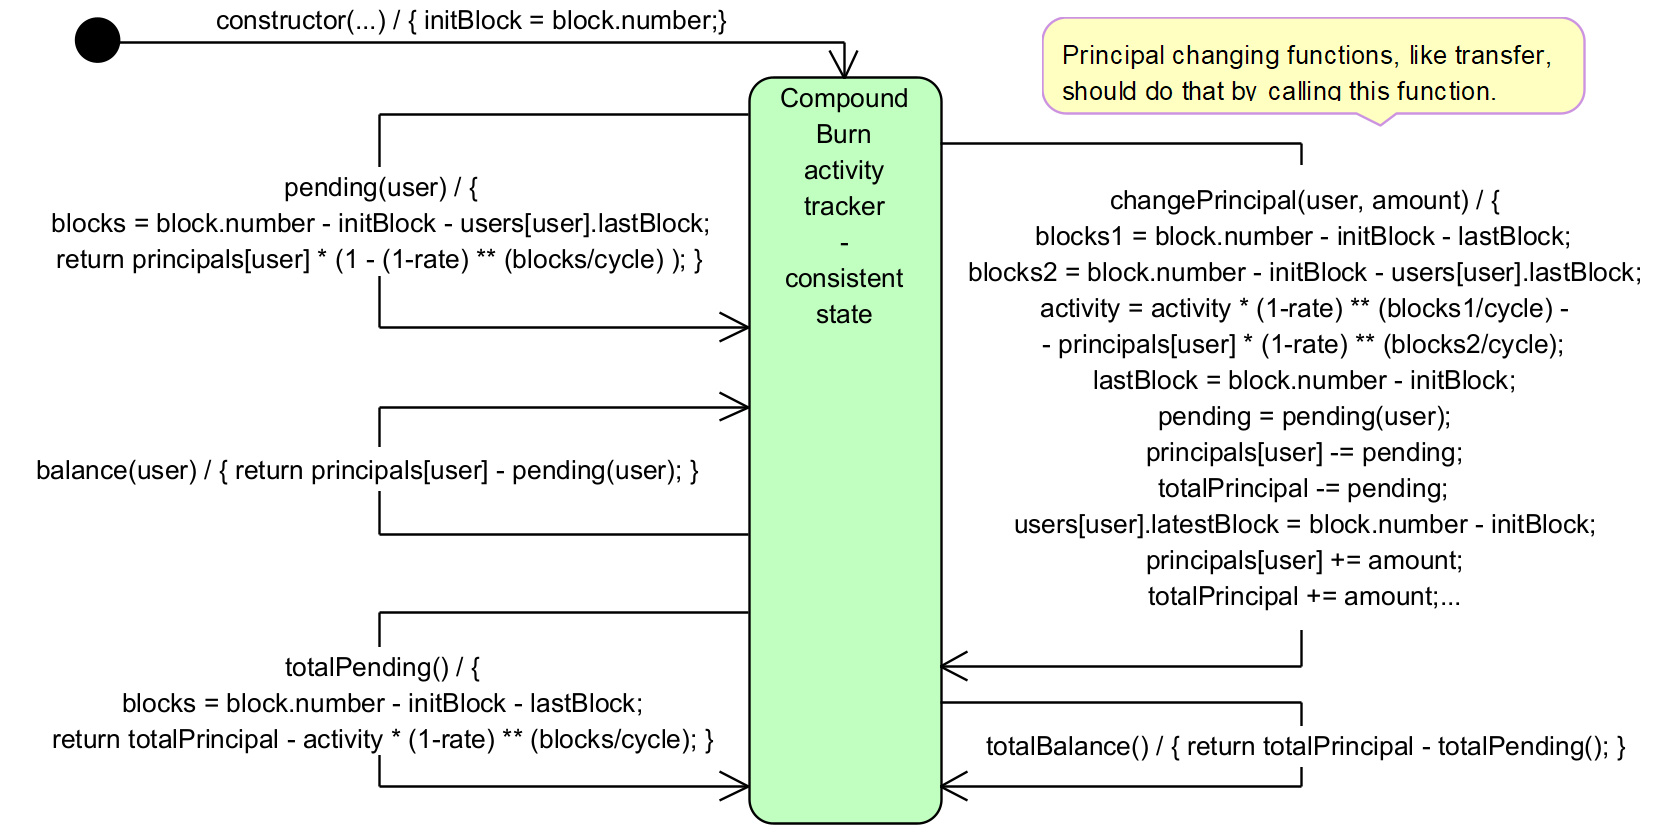
\includegraphics[width=5.3in]{images/CompoundBurnActivity.jpg}
  \caption{The UML State Machine of Compound Burn activity tracker algorithm.}
  \label{fig:CompoundBurnActivity}
\end{figure}
See Equation~\ref{eq:CompoundBurn} for the formula of Compound Burn tasks.

Figure~\ref{fig:CompoundBurnActivity} shows the state machine of the 
Compound Burn \textit{activity} tracker algorithm.

Similarly to the Compound Interest activity tracker, we can prove the following properties: \\

\begin{itemize}

  \item[$\square$] $ activity^{[e+]} = \sum_{u \in U} principals[u]^{[e+]} * (1-rate )^{(B(e+)-u.lastBlock^{[e+]})/cycle}$.
  \newline

  \item[$\square$] $ activity^{[ne+]} = \sum_{u \in U} principals[u]^{[ne+]} * (1-rate )^{(B(ne+)-u.lastBlock^{[ne+]})/cycle}$.
  \newline

  \item[$\square$] { $ pending(user)^{[r]}$ returns its true value for any user $user$.}
  \newline

  \item[$\square$] { $ totalPending^{[r]} $ returns its true value.}
  \newline

\end{itemize}

These propositions can be used to prove the consistency of the algorithm by induction for 
principal-changing moments, as in Section~\ref{sec:CompoundInterestActivity}


\subsection{Random algorithms}
\label{sec:RandomAlgorithms}

The algorithms have been proved to be consistent at any moment assuming there are 
no computer numerical errors, which is not the case.
This section discusses mitigating accumulated computer numerical errors.

Losses coming from fitting exponentiation 
of real numbers into a quotient of unsigned integers are exponentiation errors, 
while losses coming from fitting division of integers into 
an unsigned integer are division errors.
We propose an idea of improved algorithms that can 
mitigate accumulated division errors below.

See Listing~\ref{lst:Biasing} for how we identify and handle numerical errors 
in our Solidity implementation of algorithms.
\newline

\begin{lstlisting}[
  label=lst:Biasing,
  % float,
  caption={Handling division errors in our Solidity implementation of algorithm. 
  We identify two numerical error sources: the exponentiation error and 
  the division error. When $rate = 0.000474$, the whole 377,000 accumulated 
  exponentiation errors are collectively small enough if users change their 
  principal frequently and, so, if their exponents are small.
  As for the division errors, we adopt a technique that alternatingly chooses 
  between a quotient biased to a smaller value and a quotient biased to a larger 
  value, allowing the hidden division errors to cancel each other.
}
]
function pending(address user) public view returns () { 
  uint pending = 0;
  
  uint blocks = block.number - initBlock - users[user].lastBlock
  
  if (blocks > 0) {
      # Exponentiation error source: p/q = (1+r)**(blocks/cycle), r = rate / scale.
      (uint p, uint q) = analyticMath.pow(scale + rate, scale, blocks, cycle);

      # Division error source:
      pending = principals[user] - principals[user] * p / q;

      # We handle the division error source by replacing it with this alternating block.
      if (block.number % 2 == 0) {
          pending = principals[user] - IntegralMath.mulDivF(principals[user], p, q);
      } else {
          pending = principals[user], IntegralMath.mulDivC(principals[user], p, q);
      }
      # mulDivF, or multiply_and_divide_returning_floor, returns left-biased quotients, 
      # while mulDivC, or multiply_and_divide_returning_ceiling, returns right-biased quotients.
  }

  return pending; # The returned values are accumulated to balance(user)
}
\end{lstlisting}

There are two types of numerical errors for our algorithms 
when computers are operating in \textit{integers}, as is the case in Solidity programing language:
\begin{itemize}
  \item Exponentiation. 
  \newline Exponentiation errors come in two folds:
  \begin{itemize}
    \item[$\diamond$] Interest exponentiation errors: $|(1+r)^{blocks/cycle} - \{(1+r)^{blocks/cycle}\}|$
    \item[$\diamond$] Burn exponentiation errors: $|(1-r)^{blocks/cycle} - \{(1-r)^{blocks/cycle}\}|$
  \end{itemize}
  \item Division error.
  \newline
  $|i / j - \{i / j\}|$ for any positive integers $i$ and $j \neq 0$.
\end{itemize}
where $\{operation\}$ means the, theoretically existing, true return value of 
the computer operation $operation$, whereas $operation$ means the actual 
return value of the computer operation $operation$.
The true value is achieved only if there are no numerical errors, 
which is often not the case.
\newline

In order to mitigate exponentiation errors, 
we incorporate a 3rd-party mathematics library, 
called \textit{AnalyticMath}, as shown in Listing~\ref{lst:Biasing}.

The library is used as follows:
\begin{lstlisting}
  (p, q) = analyticMath.pow(a, b, c, d) 
\end{lstlisting}
for unsigned integers $a$, $b$, $c$, $d$, $p$ and $q$,
where $p$ and $q$ are intended to satisfy:
\begin{lstlisting}
  {p / q} is as close to {(a / b) ^ (c / d)} as possible
\end{lstlisting}
The provider of the library analyticMath assures that their 
found $p$ and $q$ only satisfy:
\begin{lstlisting}
If a > b, then {p / q} < {(a / b) ^ (c / d)}
If a < b, then {p / q} > {(a / b) ^ (c / d)}
\end{lstlisting}

Errors that are always less than zero or always larger than zero, 
like exponentiation errors, 
have no chance to cancel each other when they are accumulated.
Our algorithms demonstrate that 377,000 exponentiation errors, 
accumulated through the same number of transactions, 
give an insignificant collective error when exponents are small. 
Exponents are usually small if most users change their principal frequently.

Exponentiation errors are discussed more in Section~\ref{sec:Tests}, where 
test results suggest an intuition of exponentiation error as follows:
\begin{equation} \label{eq:ExponentiationError_intuision}
  | \{p / q\} - \{(a / b) ^ {(c / d)}\} | = \{alpha * (a / b) ^ {(c / d)}\}
\end{equation}
for some small constant $alpha$. 

We leave mitigating exponential errors 
over an extensively long operation and an extremely large number of transactions, 
to future research, because it requires significantly more work.

In order to mitigate division errors:

\begin{itemize}
  \item We choose a 3rd party integer division algorithm, 
  rather than Solidity's unsigned integer division. The $IntegralMath$ library 
  provides $mulDivF$ and $mulDivC$ operations, which, respectively, returns 
  the floor integer and ceiling integer of $\{integerA * integerP / integerQ\}$.
  \item We then alternatingly choose between $mulDivF$ and $mulDivC$, or between 
  a negatively biased value and a positively biased value, 
  so that the errors can cancel each other when they are accumulated 
  to $balance(user)$ throughout the application's operation.
\end{itemize}

After some mathematical work, we can achieve the following equations:

\begin{itemize}
  \item If $\sum_{u \in U} balance(u)$ is evaluated with Solidity's floor-returning integer division, 
  and if N denotes the number of accumulation of $pending(user)$, then
    \begin{equation} \label{eq:NativeDivision}
    N/4 < \mathbb{E} (| \sum_{u \in U} balance(u) - \{ {\sum_{u \in U} balance(u)} \} |) < N
    \end{equation}
    \item If $\sum_{u \in U} balance(u)$ is evaluated with the 3rd-party alternating integer divisions, then
    \begin{equation} \label{eq:3rdPartyDivision}
      \mathbb{E} (| \sum_{u \in U} balance(u) - \{ {\sum_{u \in U} balance(u)} \} |) \le 1
    \end{equation}
\end{itemize}
where $\mathbb{E}$ denotes the expected value and $N$ is the number of principal-changing transactions.
Equation~\ref{eq:NativeDivision} indicates that the floor-returning integer division gives errors 
that diverge slowly linearly, while Equation~\ref{eq:3rdPartyDivision} means the alternating 
integer divisions give errors that converge to zero, both in an appropriate meaning.
As for $totalBalance()$, the proof should be similar as for $\sum_{u \in U} balance(u)$.

Algorithms that mitigate division errors by using the 3rd-party alternating integer divisions 
are called \textbf{random algorithms}. 
In random algorithms, the long-term behavior of 
errors should solely be determined by the exponentiation error source.
See Table~\ref{tbl:AlgorithmsClassified} for the classification of algorithms.
\newline
\begin{table} [H]
% \begin{center}
  \begin{spacing}{1.8}\centering
    \fontsize{8pt}{8pt}\selectfont
    \begin{tabular} {|m{3cm} |m{5cm} |m{6cm} |}
    \hline
    {\textbf{Task type}} & {\textbf{Algorithms that don't handle errors}} & {\textbf{Random algorithms that handle division errors}} \\
    \hline
    {\textbf{Simple Interest}} & 
    {Simple Interest Pendency tracker} \newline {Simple Interest Activity tracker} &  
    {Simple Interest Pendency random tracker} \newline {Simple Interest Activity random tracker} \\[3mm]
    \hline
    {\textbf{Simple Burn}} &
    {Simple Burn Pendency tracker} \newline {Simple Burn Activity tracker} &  
    {Simple Interest Burn random tracker} \newline {Simple Burn Activity random tracker} \\[3mm]
    \hline
    {\textbf{Compound Interest}} &
    {Compound Interest Pendency tracker} \newline {Compound Interest Activity tracker} &  
    {Compound Interest Pendency random tracker} \newline {Compound Interest Activity random tracker} \\[3mm]
    \hline
    {\textbf{Compound Burn}} &
    {Compound Burn Pendency tracker} \newline {Compound Burn Activity tracker} &  
    {Compound Interest Burn random tracker} \newline {Compound Burn Activity random tracker} \\[3mm]
    \hline
  \end{tabular}
  \end{spacing}
% \end{center}
\caption {Classification of algorithms}
\label{tbl:AlgorithmsClassified}
\end{table}

We note, however, $N$, as both 
the number of principal-changing transactions and 
the upper limit of accumulated division errors, 
is 
a \textit{negligibly small} number compared to the magnitude of $totalBalance()$.
Looking at the existing busiest DeFies, 
the total number of transactions during their past existence 
is less than a couple of millions ($10^6$),
while the magnitude of $totalBalance()$, 
which acts as the denominator in Relative Errors A and B, 
is usually over $10^{18+5}$. 
This means the accumulated division errors will have trivial effect 
on \textit{Relative} Consistency Errors, 
which is the main performance measure.
Therefore the random algorithms will \textit{not} 
give a significant improvement of accuracy, 
if we don't have extensively many transactions.
We just propose random algorithms and do not concentrate on them in our test, 
as our future work is expected to concentrate on errors.

\section{Tests}
\label{sec:Tests}

See Section~\ref{sec:Tasks} for the definitions of task types.
See Section~\ref{sec:Pendency_vs_Activity} for the concepts of 
pendency and activity.
See Section~\ref{sec:RandomAlgorithms} for random algorithms.

We perform simple stress tests for them, for the \textit{purpose} of checking 
if the algorithms can operate in \textit{diversified environments} 
for \textit{longer periods} and \textit{consistently.}
The diversity is achieved by using randomly generated transactions 
in various test modes, 
the longevity is tested by running tests a long time, and 
the consistency is checked by using our Consistency Criteria defined 
in Section~\ref{sec:Criteria}.
The single most important concept in testing is Consistency Errors, 
defined in Equation~\ref{eq:TrueTotal} through Equation~\ref{eq:AbsoluteErrorB}.

\subsection{Baseline}
\label{sec:javascriptTruth}

We introduce $javascriptTruth$ and $solidityTruth$ for testing our algorithms.
Our tests aim to assess Consistency Errors, which by and large come from 
accumulating $pending(user)$, $pendency$, and $activity$. Exponentiation errors 
and division errors identified above, which are trivial individually, 
should be concerned because they are accumulated over transactions, 
with their values biased harmfully in a single direction.
For example, $totalBalance()$ is essentially an accumulation formulated as 
\begin{equation} \label{eq:AccumulatedTotalBalance_Compound}
  totalBalance()_{i} = totalBalance()_{i-1} * (1+rate)^{(B(e_{i}+)-B(e_{i-1}+))/cycle},
\end{equation}
in Compound Interest tasks, where $e_{i}$ is $i^{th}$ principal-changing events.
Every round of the successive accumulation brings a numerical error into $balance(user)$ 
and $totalBalance()$, and the errors are harmfully biased in a single direction 
not canceling each other.
If there are no numerical errors, then Equation~\ref{eq:AccumulatedTotalBalance_Compound} 
can be simplified to:
\begin{equation} \label{eq:ShortcutTotalBalance_Compound}
  \begin{split}
  totalBalance()_{i} = totalBalance()_{0} * (1+rate)^{(B(e_{i}+)-B(e_{0}+))/cycle}
  \end{split}
\end{equation}

In Simple Interest tasks, the corresponding two equations are, respectively:
\begin{equation} \label{eq:AccumulatedTotalBalance_Simple}
  totalBalance()_{i} = InitTotal * \sum_{i=1}^{N} (1+rate) * (B(e_{i}+)-B(e_{i-1}+))/cycle
\end{equation}
\begin{equation} \label{eq:ShortcutTotalBalance_Simple}
  \begin{split}
  totalBalance()_{i} = InitTotal * (1+rate) * {(B(e_{N}+)-B(e_{0}+))/cycle}
  \end{split}
\end{equation}

The Equations \ref{eq:AccumulatedTotalBalance_Compound} and \ref{eq:AccumulatedTotalBalance_Simple} 
are a \textit{return value} of the algorithms, while Equations
\ref{eq:ShortcutTotalBalance_Compound} and \ref{eq:ShortcutTotalBalance_Simple}, 
which have no accumulation, 
are almost free of error and very near the \textit{true value} of query $totalBalance()$.
We use Equations
\ref{eq:ShortcutTotalBalance_Compound} and \ref{eq:ShortcutTotalBalance_Simple} 
as a substitute for $TrueTotal$ defined in 
Equation~\ref{eq:TrueTotal}, in their respective task types.
To further reduce errors, we calculate the $TrueTotal$'s substitutes in Javascript 
programing language, rather than in Solidity language, which operates in unsigned integers 
creating larger errors. 
The Javascript version of the $TrueTotal$'s substitutes is called 
$javascripTruth$ below. For the comparison purpose, we also have the Solidity version of 
$TrueTotal$'s substitutes and call them $solidityTruth$.
\newline

\subsection{Testing Procedure}
\label{sec:TestingProcedure}
To generate simulated diversified environments, we create an automatic testing 
program that acts as follows:

\begin{itemize}
  \item Four simulated users - Owner, Alice, Bob, and Carol; are created on a private 
  block chain, each with enough cryptocurrency for gas fee payment.

  \item A smart contract that implements the target algorithm, as well as the 
  four queries in Consistency Criteria, is deployed on the block chainwork, with 18 
  decimal places as usual. See Section~\ref{sec:Criteria} for Consistency Criteria.

  \item The smart contract implements transfer, mint, and burn functions on the principal 
  amount of users, by using the $changePrincipal(user, amount)$ function offered 
  by the algorithm.

  \item The smart contract's constructor mints $10^8$ tokens to Owner as the initial 
  amount for the principal of Owner. An interest/burn rate of 0.0474 \% 
  a simulated day is assumed, which is equivalent to 1 \% interest every 21 days 
  in Compound Interest tasks.
  One simulated day spans 10 blockchain blocks.

  \item $transfer$, $mint$, and $burn$ transactions (called simply a function below) 
  are raised randomly from the off-chain part with randomly chosen arguments, 
  like $user$ and $amount$, while the $mintBlocks$ function is called intermittently 
  to advance the block number (or, the internal time) in the block chain, 
  again with a randomly chosen number of blocks to advance.
  Fixed probability distributions over the functions' occurrences, 
  over $user$, and over $amount$, respectively, are assumed.

  Once a randomly chosen function is called, the function repeatedly tries 
  randomly changing $user$ and $amount$, up to 50 times  
  until it succeeds, thus adhering to the given 
  probability distribution over function occurrences.
  We note the $transfer$ transaction, for example, may well 
  fail, because the principal amounts for all users may become almost zero 
  after a Compound Burn task runs a long time with a significant burn rate.

  \item Typically, 200,000 calls are made in a test. $Transfer$ transactions 
  account for 90 \% of the total calls, and the remaining part is accounted for 
  by $mint$, $burn$, and $mintBlocks$. 
  In each test, up to 468,000 blocks representing 46,800 simulated days or 
  128 simulated years are minted by $mintBlocks$ calls. 
  1 to 50 blocks are minted by a $mintBlocks$ call, representing 1 tenth day to 
  5 days minted by a $mintBlocks$ call.

  \item As random functions are called, the smart contract and testing program 
  cooperate to calculate $solidityTruth$, $javascripTruth$, and Consistency Errors.
  Sec Section~\ref{sec:javascriptTruth} for $solidityTruth$ and $javascripTruth$, 
  and Section~\ref{sec:Criteria} for Consistency Errors.
  \newline
\end{itemize}

The testing program has two modes: Free Total Principal test mode and Fixed Total Principal test mode.

\label{sec:TestModes}

\begin{itemize}
  \item {Free Total Principal test mode}  \newline

  In this mode, the testing program does not call $mint$ and $burn$ transactions, 
  leaving the total principal or reward amount to freely change according 
  to their formulas shown in Section~\ref{sec:Tasks}.

  \begin{figure}[H]
    \centering
    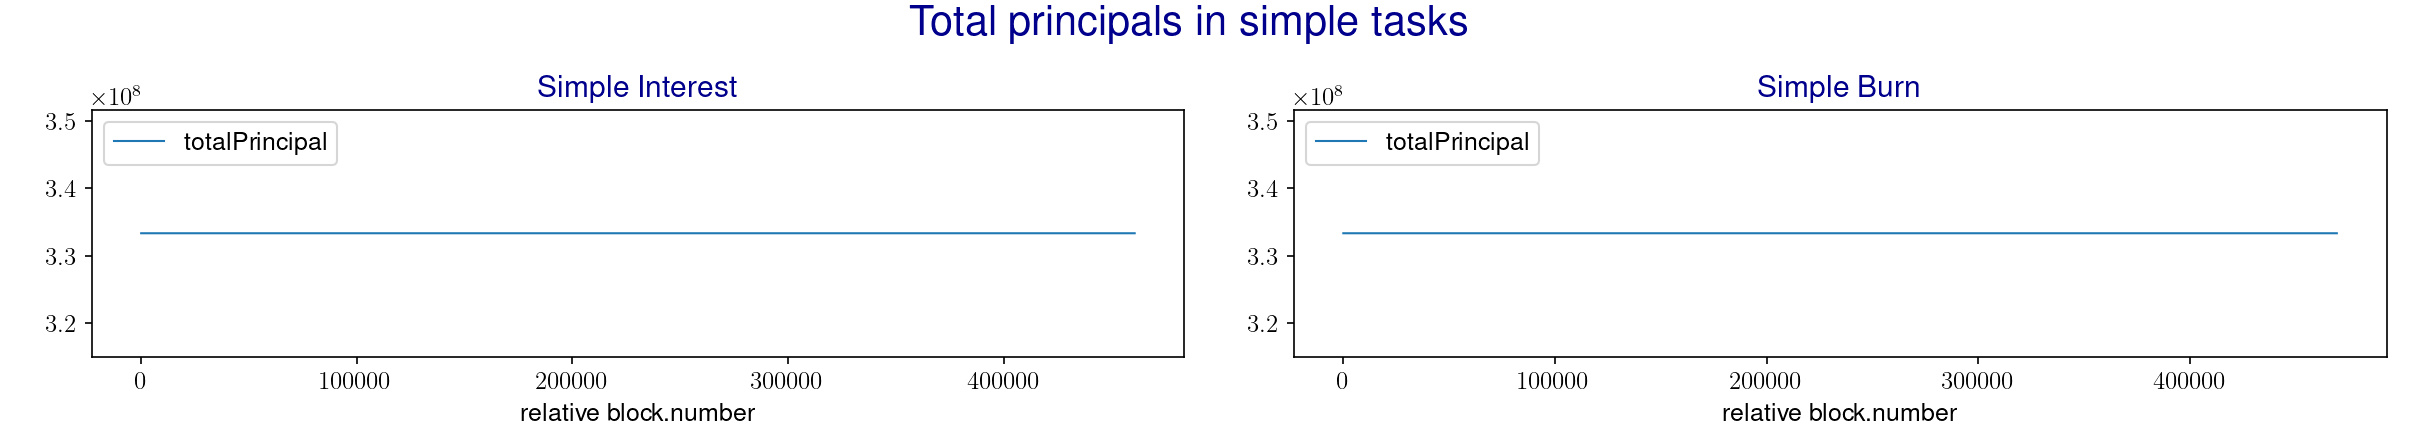
\includegraphics[width=5.3in]{images/_6.3_sim_total_principal.jpg}
    \caption{For a simple task in the Free Total Principal test mode, 
    $totalPrincipal$ keeps constantly to its initial value.
    }
    \label{fig:fixed_sim_pillars_mode_free}
  \end{figure}

  \begin{figure}[H]
    \centering
    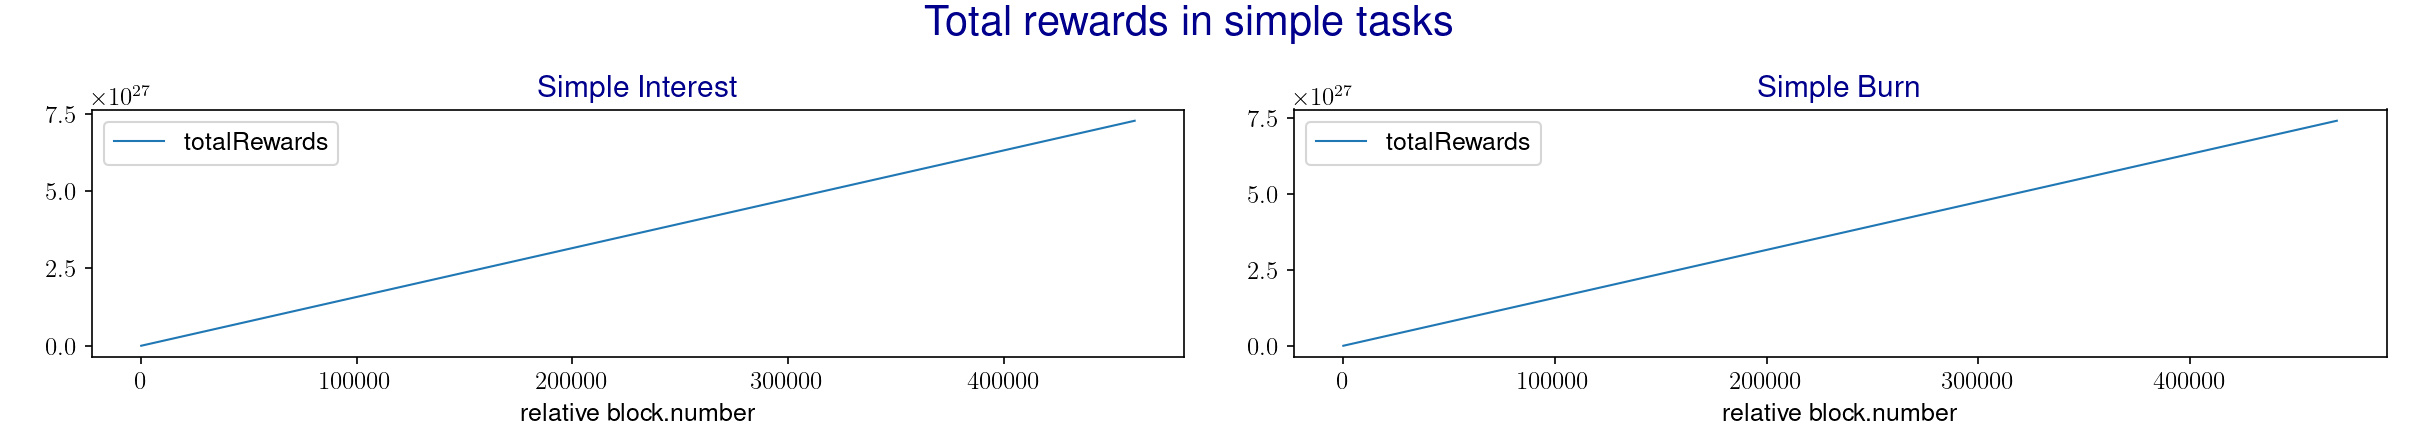
\includegraphics[width=5.3in]{images/_6.3_sim_total_rewards.jpg}
    \caption{For a simple task in the Free Total Principal test mode, 
    $totalRewards$ grows freely linearly, 
    because the time-linear interest or burn is additively 
    accumulated to $reward[user]$.
    }
    \label{fig:fixed_sim_pillars_mode_free}
  \end{figure}

  \begin{figure}[H]
    \centering
    % \fbox{\rule[-.5cm]{4cm}{4cm} \rule[-.5cm]{4cm}{0cm}}
    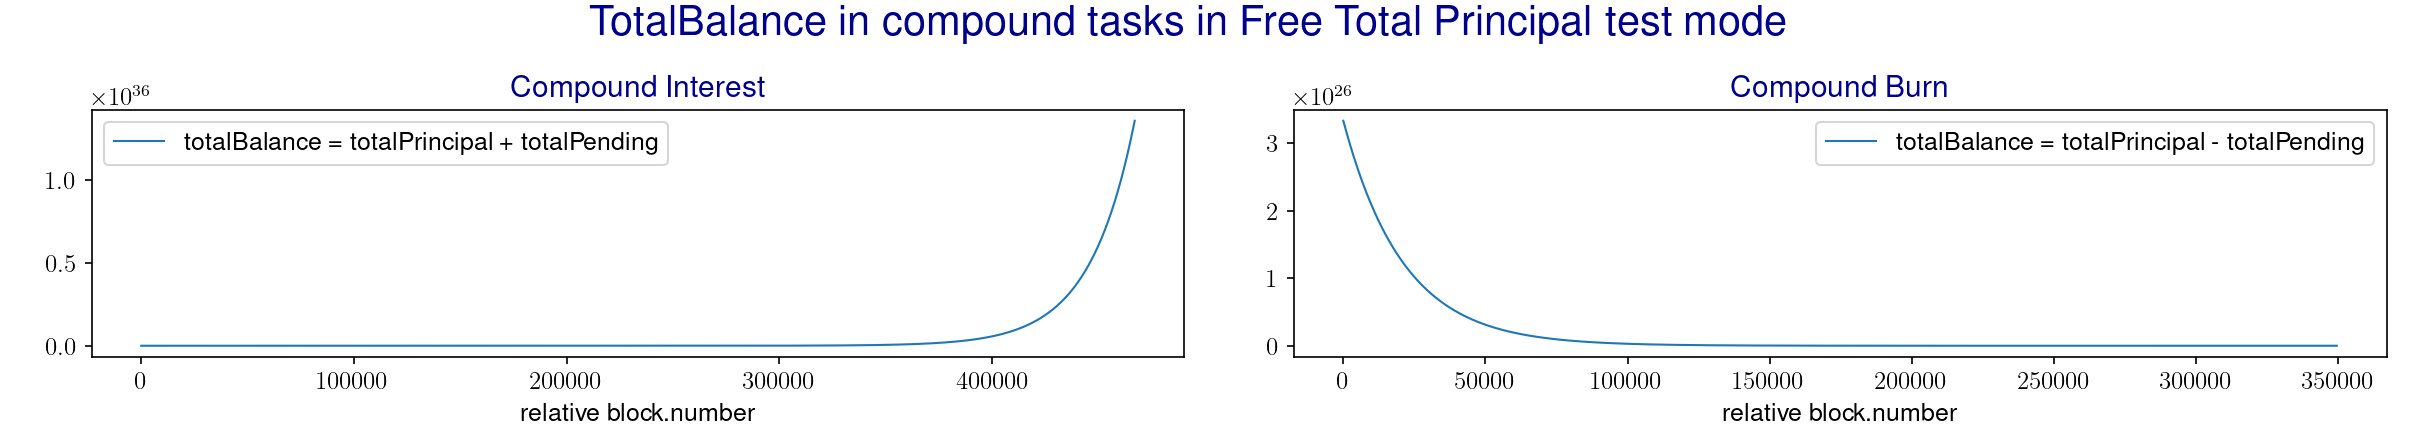
\includegraphics[width=5.3in]{images/_6.3_free_com_total_balance.jpg}
    \caption{$totalBalance()$ for compound tasks in 
    Free Total Principal test mode grows/shrinks freely exponentially 
    from its initial total principal 
    as much as time goes and $rate$ allows,
    because the 
    time-exponential interest/burn \textit{is} compounded to/from $principals[user]$.
    }
    \label{fig:free_com_total_mode}
  \end{figure}
  
  We note $TrueTotal$, defined in Equation~\ref{eq:TrueTotal}, acting as the denominator 
  in Relative Errors A and B, may get extremely large in a Compound Interest tasks
  or get extremely small in a Compound Burn task, 
  affecting the Relative Errors to diminish or diverge (unless their numerators  
  change faster in the same direction.)
  This mode aims to simulate an extreme operation where the total principal is 
  not managed/limited by system administrators and observe how consistent the algorithms 
  are in those harsh conditions.  \newline

  \item {Fixed Total Principal test mode}   \newline

  In this mode, the testing program resists change of total principal by 
  choosing a suitable value for the $amount$ argument of randomly called  
  $mint$ or $burn$ transactions.
  The incremental changes to the total principal amount 
  in Compound Interest tasks or the decremental changes of the total principal 
  in Compound Burn 
  tasks are compensated by the suitable $amount$ arguments 
  passed to the $mint$ or $burn$ transactions, keeping the total principal 
  to its initial value.

  \begin{figure}[H]
    \centering
    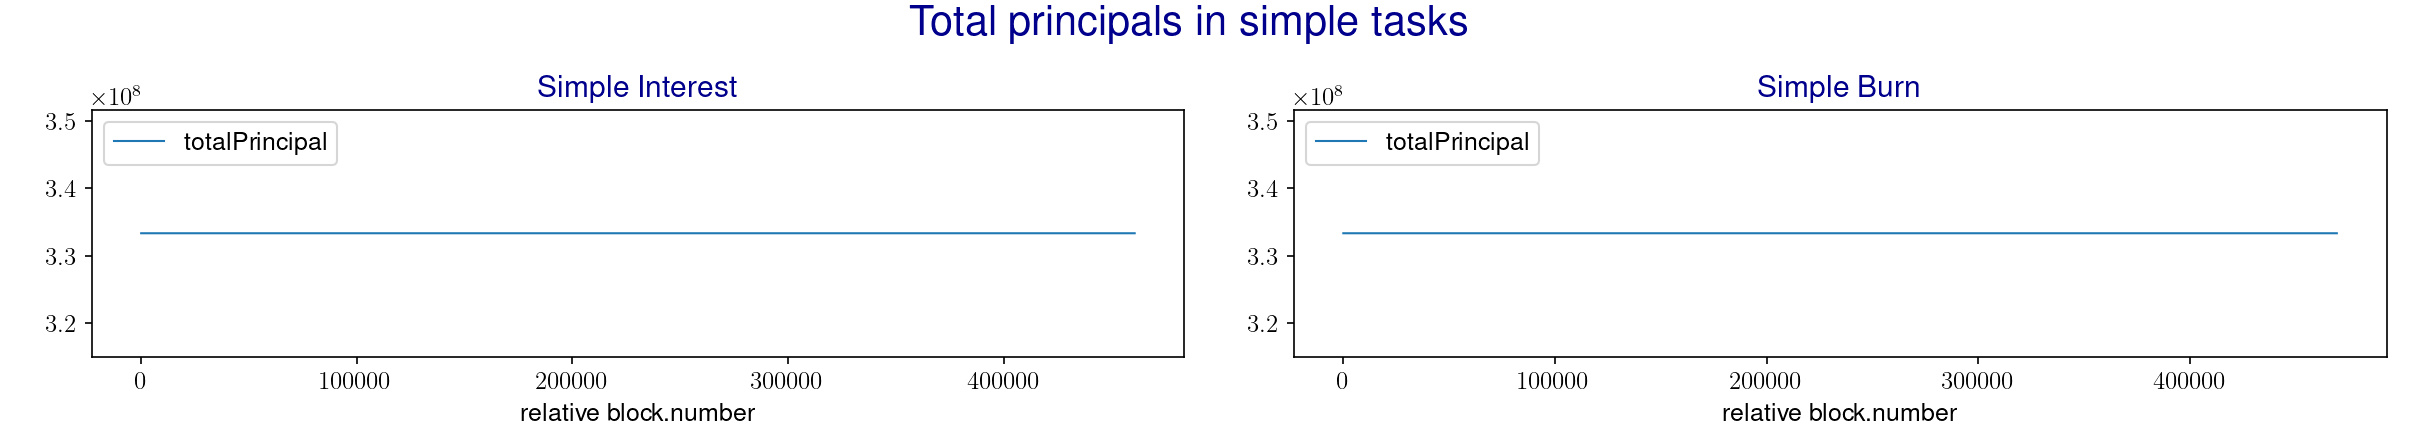
\includegraphics[width=5.3in]{images/_6.3_sim_total_principal.jpg}
    \caption{For a simple task in the Fixed Total Principal test mode, 
    $totalPrincipal$ keeps constant to its initial value.
    While the testing program tries to keep $totalPrincipal$ fixed    
    (with $mint$ or $burn$ transactions from offchain),
    every $principals[user]$, so $totalPrincipal$ too, is already fixed, 
    because the (linear) interest or burn is \textit{not} 
    compounded to $principals[user]$.
    }
    \label{fig:fixed_sim_pillars_mode_fixed}
  \end{figure}

  \begin{figure}[H]
    \centering
    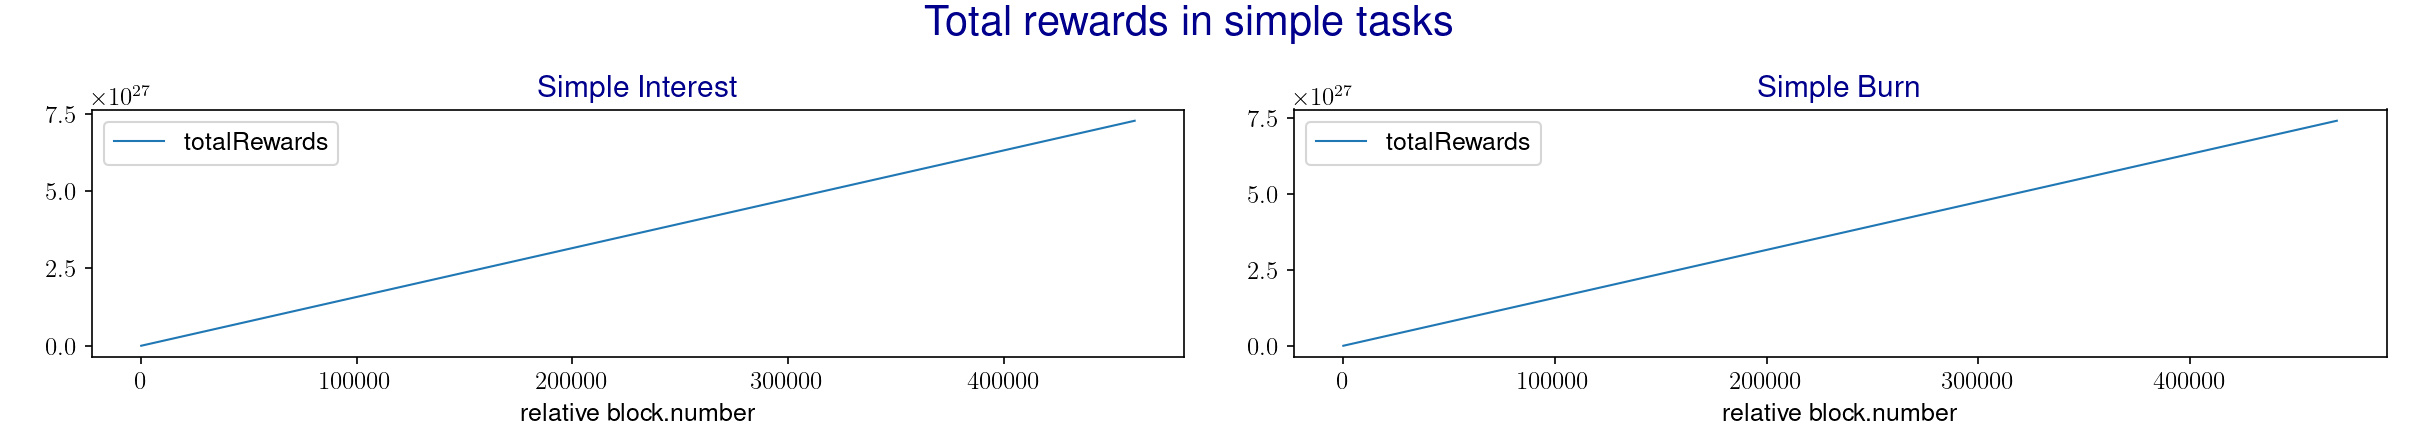
\includegraphics[width=5.3in]{images/_6.3_sim_total_rewards.jpg}
    \caption{For a simple task in the Fixed Total Principal test mode,
    $totalRewards$ grows freely linearly, 
    because the 
    linear interest or burn is additively accumulated to $reward[user]$.
    }
    \label{fig:fixed_sim_pillars_mode_fixed}
  \end{figure}

  \begin{figure}[H]
    \centering
    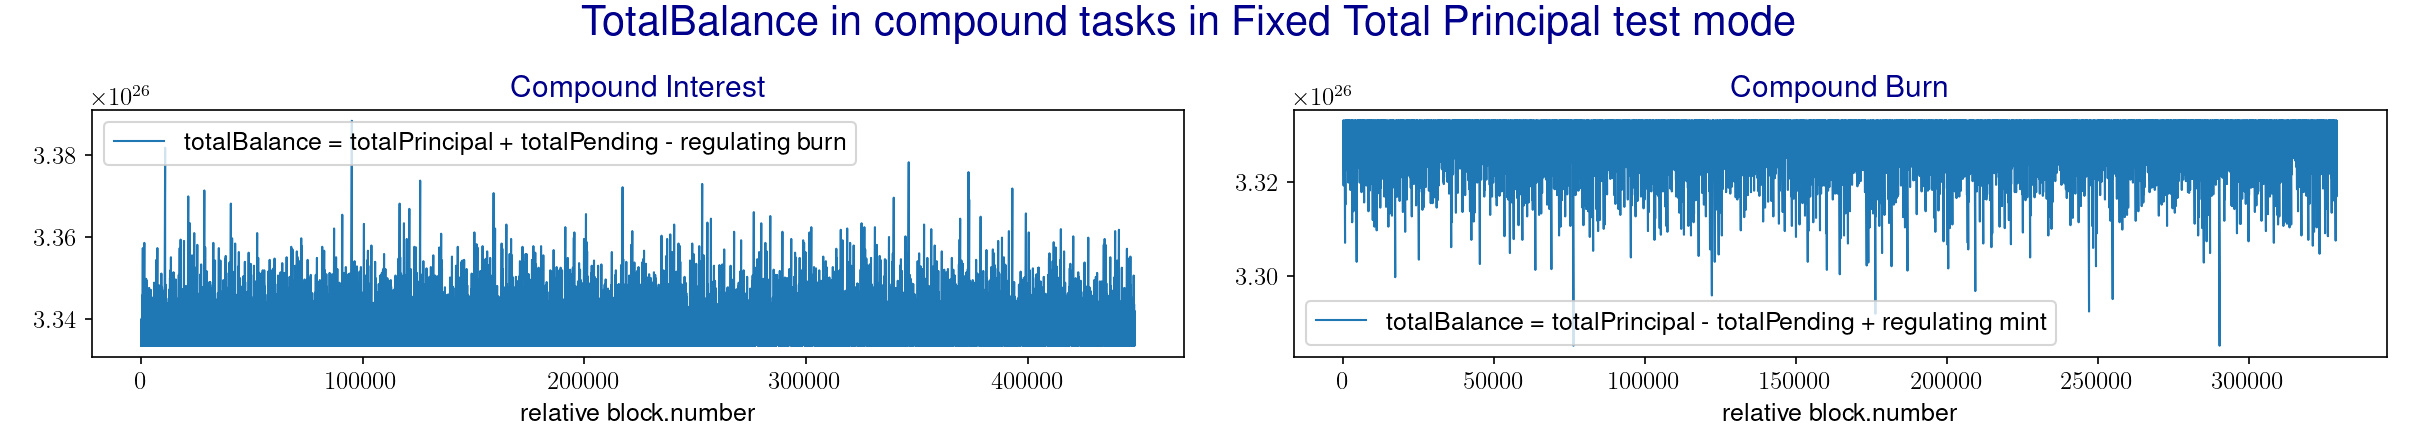
\includegraphics[width=5.3in]{images/_6.3_fixed_com_total_balance.jpg}
    \caption{For compound tasks in the Fixed Total Principal test mode, 
    $totalBalance$  
    is regulated by the testing program with $mint$ or $burn$ transactions, 
    so that $totalBalance$ reverts to its initial value frequently.
    }
    \label{fig:fixed_com_total_mode}
  \end{figure}

  \begin{figure}[H]
    \centering
    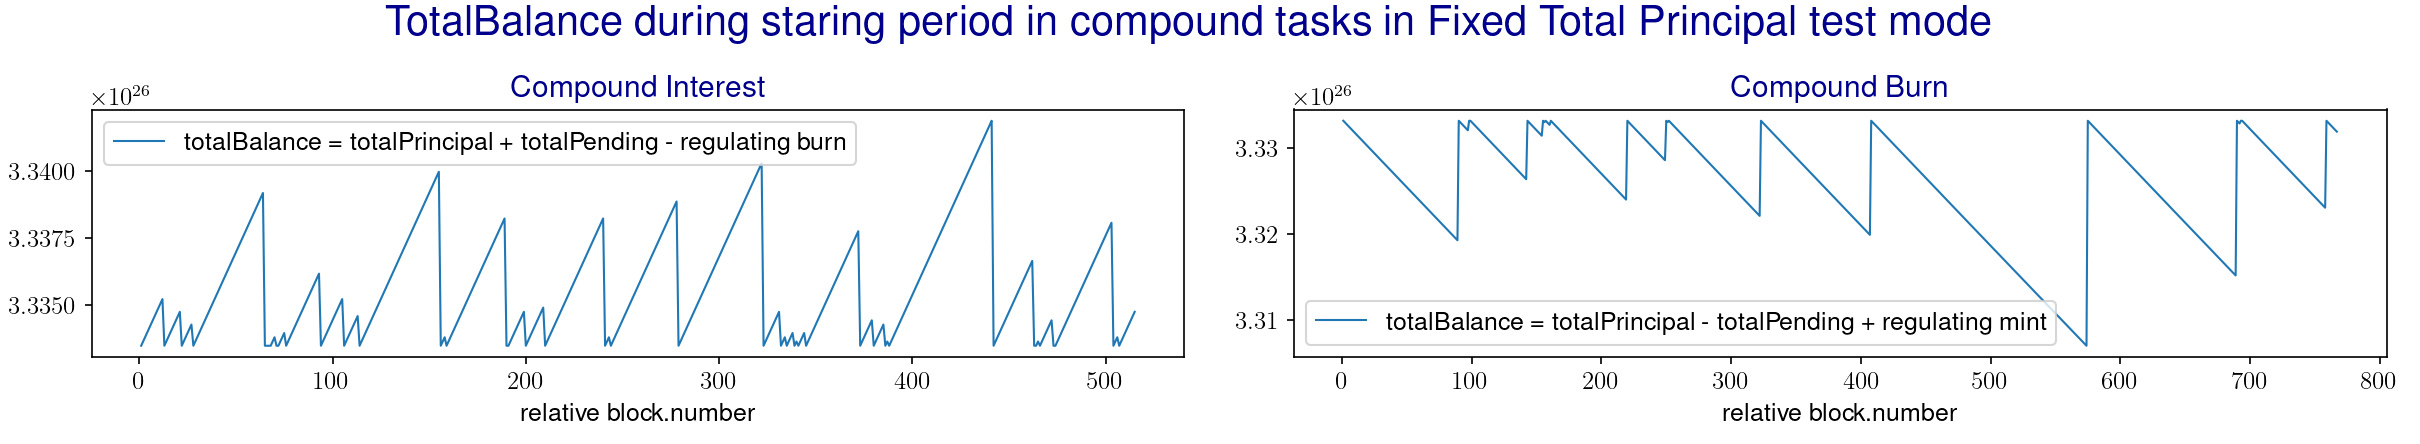
\includegraphics[width=5.3in]{images/_6.3_fixed_com_total_balance_start.jpg}
    \caption{For compound tasks in the Fixed Total Principal test mode, 
    the testing program regulates $totalBalance$, which would otherwise 
    grow/shrink freely as in Figure~\ref{fig:free_com_total_mode}, 
    by pulling it down/up to its initial value intermittently.
    }
    \label{fig:fixed_com_total_start_mode}
  \end{figure}

  This mode aims to simulate a modest operation where the total principal 
  is completely managed to be stable, as will be the case in many applications, 
  by system administrators, and confirm how consistent the algorithms 
  are in those typical conditions.

\end{itemize}

\subsection{Test cases}
\label{sec:TestCases}

Test cases are as follows:
\newline

\begin{itemize}
  \item {Simple tasks in Free Total Principal mode} \newline
  Simple tasks types, which are Simple Interest and Simple Burn, are tested 
  each in its two alternative algorithms: pendency tracker and activity tracker,
  in the Free Total Principal test mode.
  
  \item {Compound tasks in Free Total Principal mode} \newline
  Compound tasks types, which are Compound Interest and Compound Burn, are tested 
  each in its two alternative algorithms: pendency tracker and activity tracker, 
  in the Free Total Principal test mode.

  \item {Simple tasks in Fixed Total Principal mode} \newline
  Simple task types, which are Simple Interest and Simple Burn, are tested 
  each in its two alternative algorithms: pendency tracker and activity tracker, 
  in the Fixed Total Principal test mode.

  \item {Compound tasks in Fixed Total Principal mode} \newline
  Compound task types, which are Compound Interest and Compound Burn, are tested 
  each in its two alternative algorithms: pendency tracker and activity tracker, 
  in the Fixed Total Principal test mode.

\end{itemize}

\subsection{Test case: Simple Tasks in Free Total Principal mode}

\begin{figure}[H]
  \centering
  % \fbox{\rule[-.5cm]{4cm}{4cm} \rule[-.5cm]{4cm}{0cm}}
  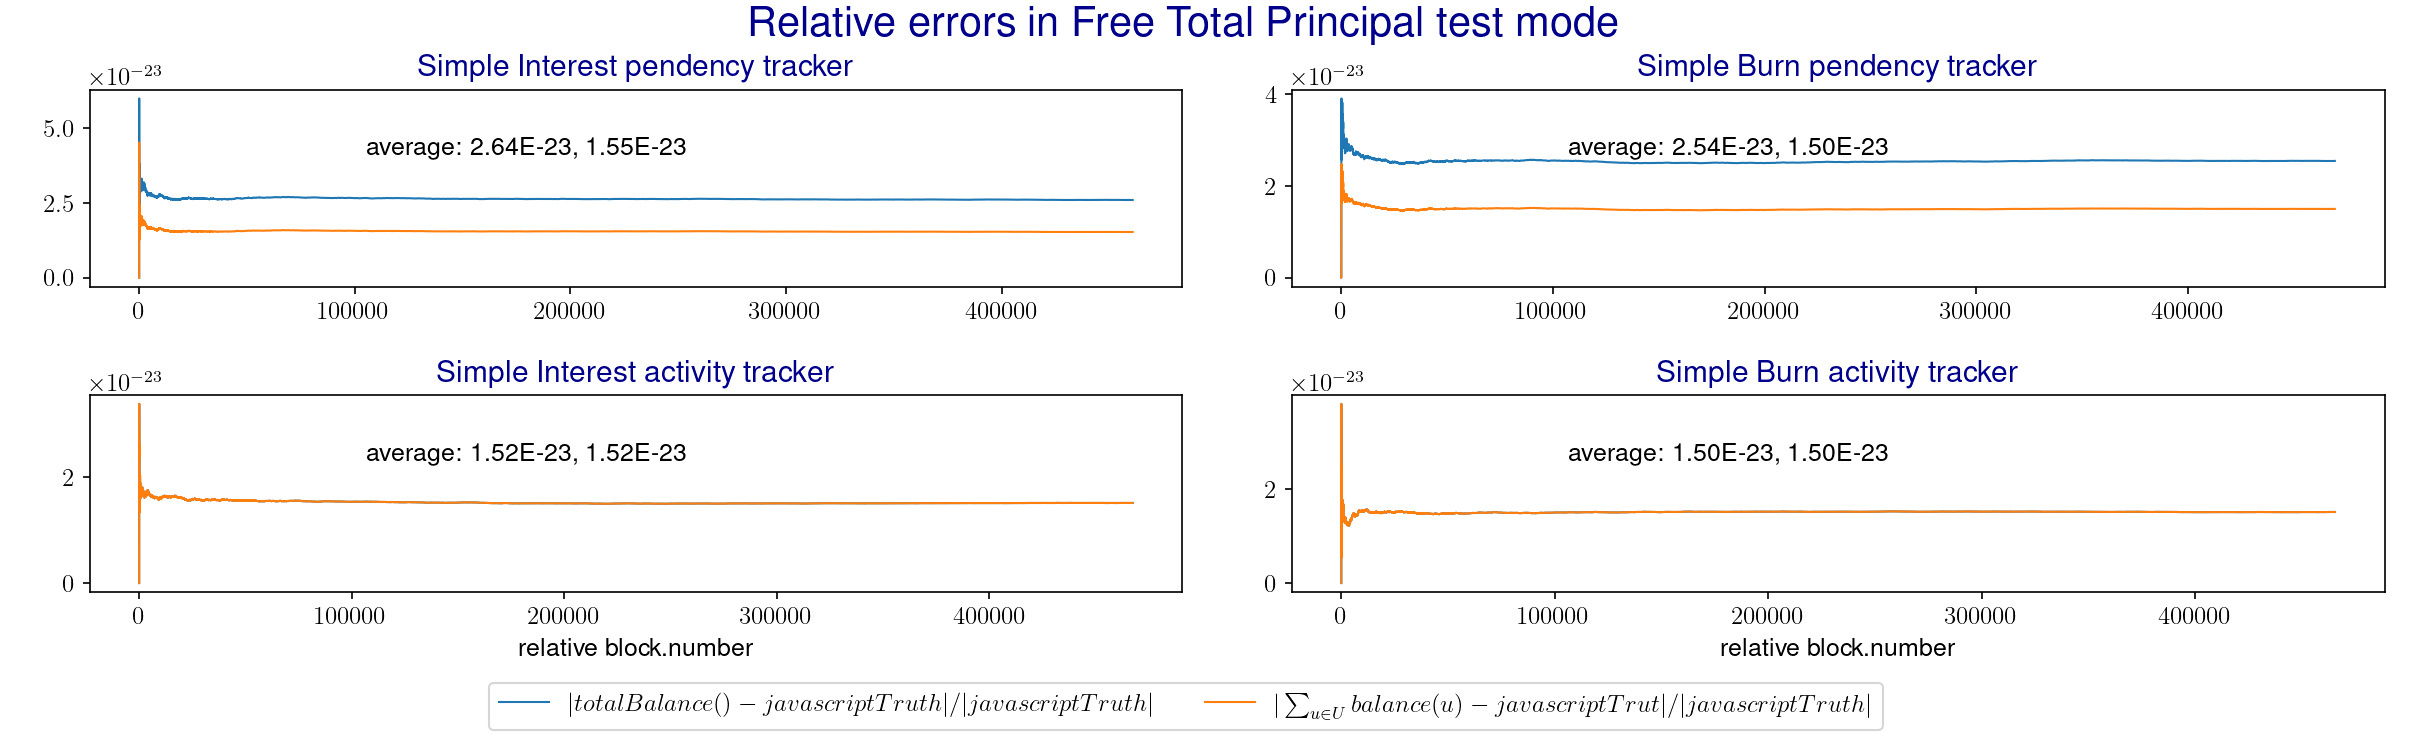
\includegraphics[width=5.3in]{images/6.3_free_sim_relative.jpg}
  \caption{Relative Errors A and B in simple tasks 
  in Free Total Principal test mode.
  The Relative Errors converge 
  and are less than $10^{-22}$ during 128 simulated years and 
  180,000 transfer transactions. 
  }
  \label{fig:free_sim_absolute_case}
\end{figure}

\begin{figure}[H]
  \centering
  % \fbox{\rule[-.5cm]{4cm}{4cm} \rule[-.5cm]{4cm}{0cm}}
  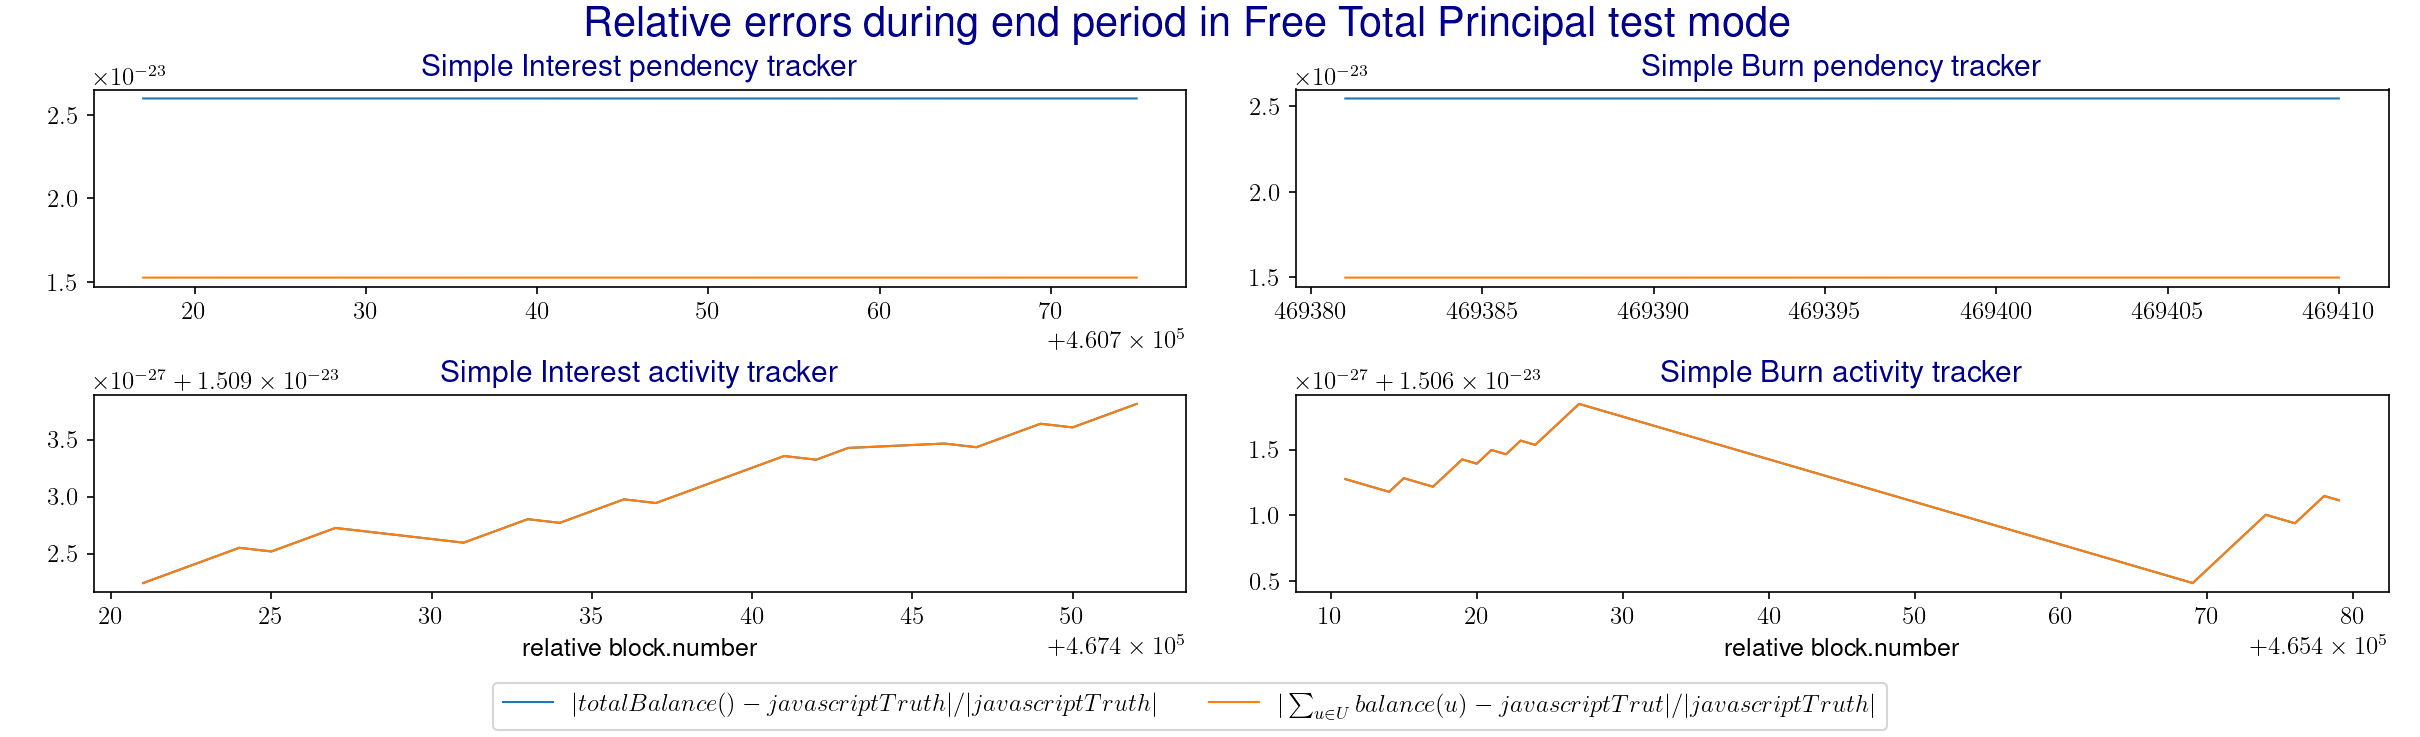
\includegraphics[width=5.3in]{images/6.3_free_sim_relative_end.jpg}
  \caption{Relative Errors A and B, after a long run, for simple tasks 
  in Free Total Principal test mode. For pendency trackers, $totalBalance$ 
  and $\sum_{u \in U}balance(u)$ reveal significant deviation from their 
  shared substitute true value $javascriptTruth$.
  For activity trackers, the two values are fluctuating. 
  }
  \label{fig:free_sim_relative_end_case}
\end{figure}

\subsection{Test case: Compound Tasks in Free Total Principal mode}

\begin{figure}[H]
  \centering
  % \fbox{\rule[-.5cm]{4cm}{4cm} \rule[-.5cm]{4cm}{0cm}}
  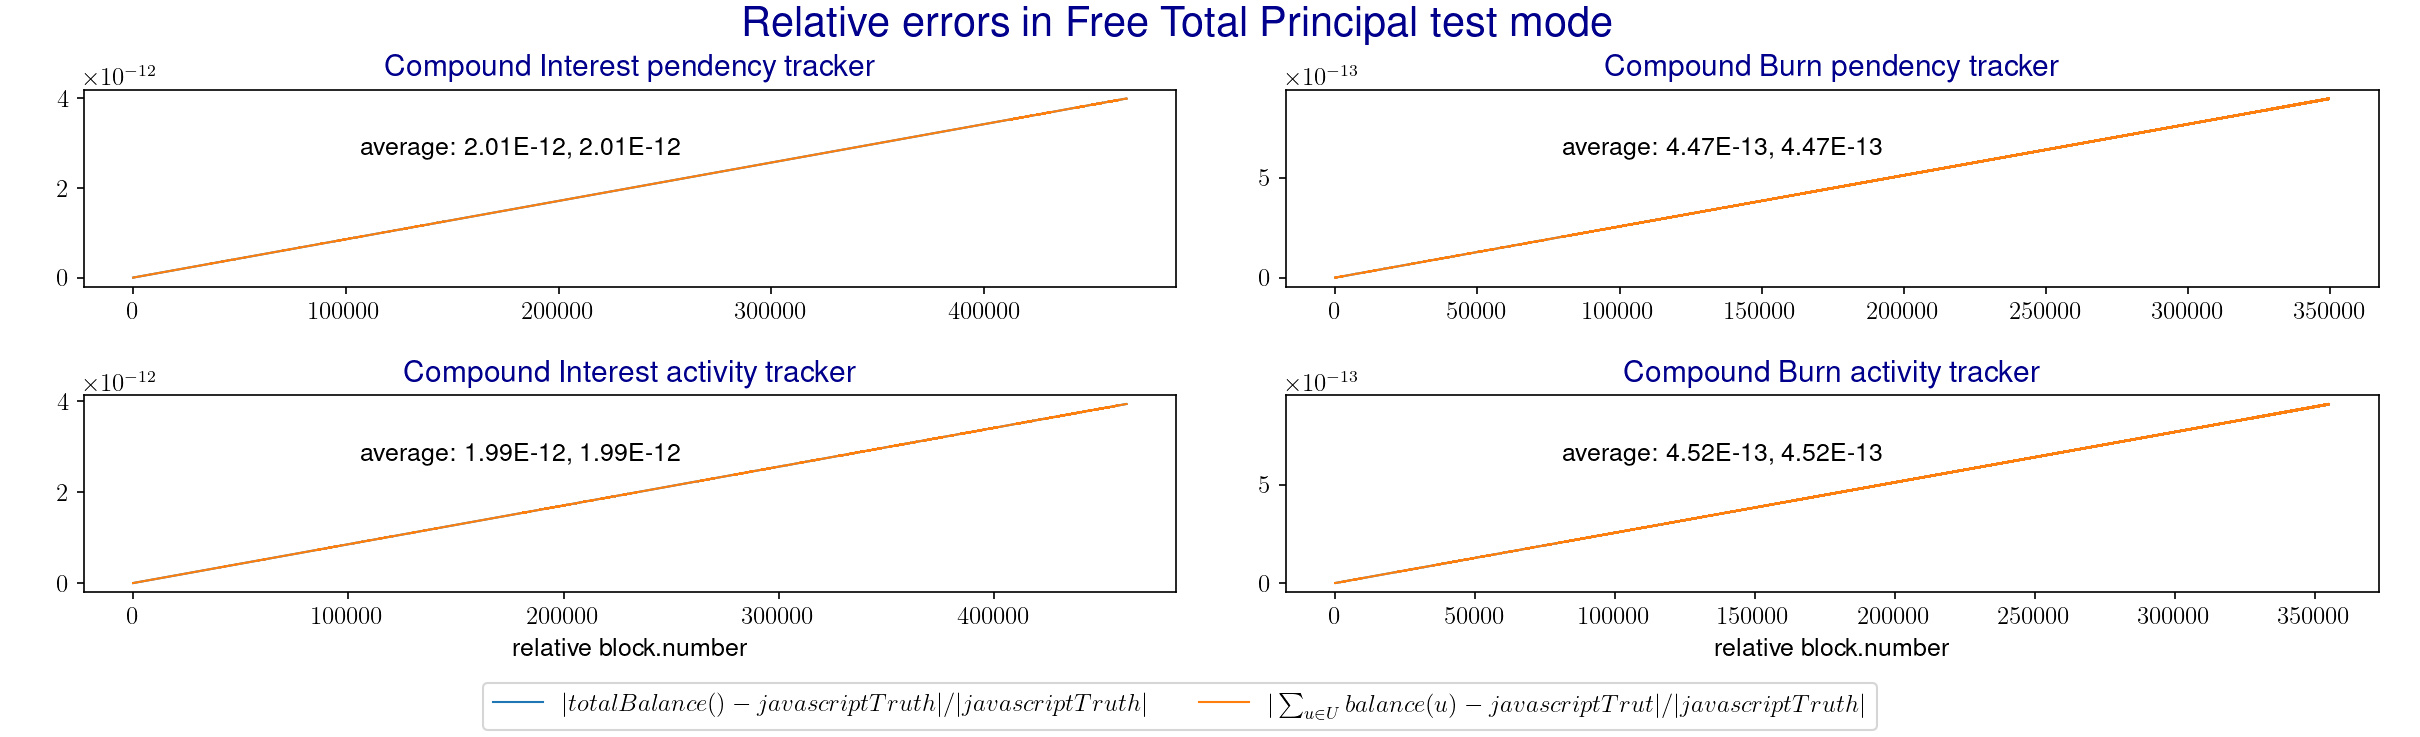
\includegraphics[width=5.3in]{images/6.3_free_com_relative.jpg}
  \caption{Relative Errors A and B for compound tasks 
  in Free Total Principal test mode. 
  The Relative Errors grow linearly over time 
  and are less than $10^{-11}$ during 128 simulated years and 
  180,000 transfer transactions.
  }
  \label{fig:free_com_relative_case}
\end{figure}

\begin{figure}[H]
  \centering
  % \fbox{\rule[-.5cm]{4cm}{4cm} \rule[-.5cm]{4cm}{0cm}}
  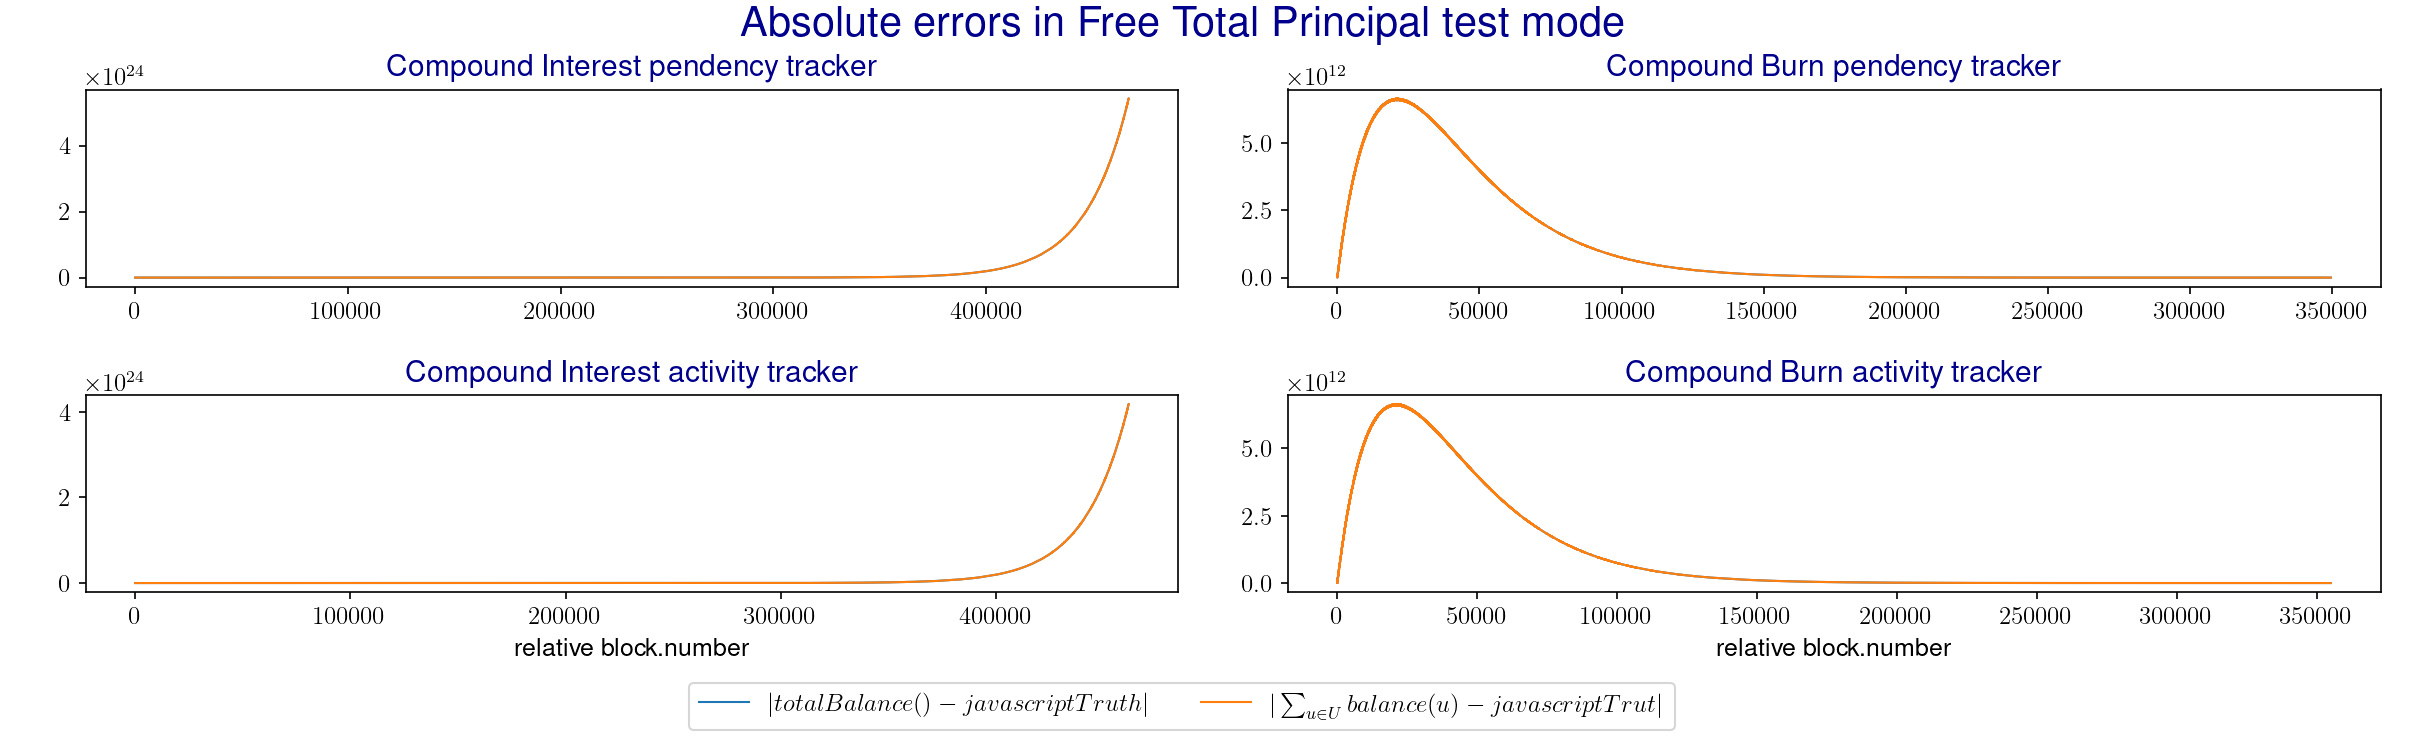
\includegraphics[width=5.3in]{images/6.3_free_com_absolute.jpg}
  \caption{Absolute Consistency Errors for compound tasks 
  in Free Total Principal test mode. They  
  have exponential growth as suggested by the linearity of Relative Errors A and B.
  }
  \label{fig:free_com_absolute_case}
\end{figure}

\begin{figure}[H]
  \centering
  % \fbox{\rule[-.5cm]{4cm}{4cm} \rule[-.5cm]{4cm}{0cm}}
  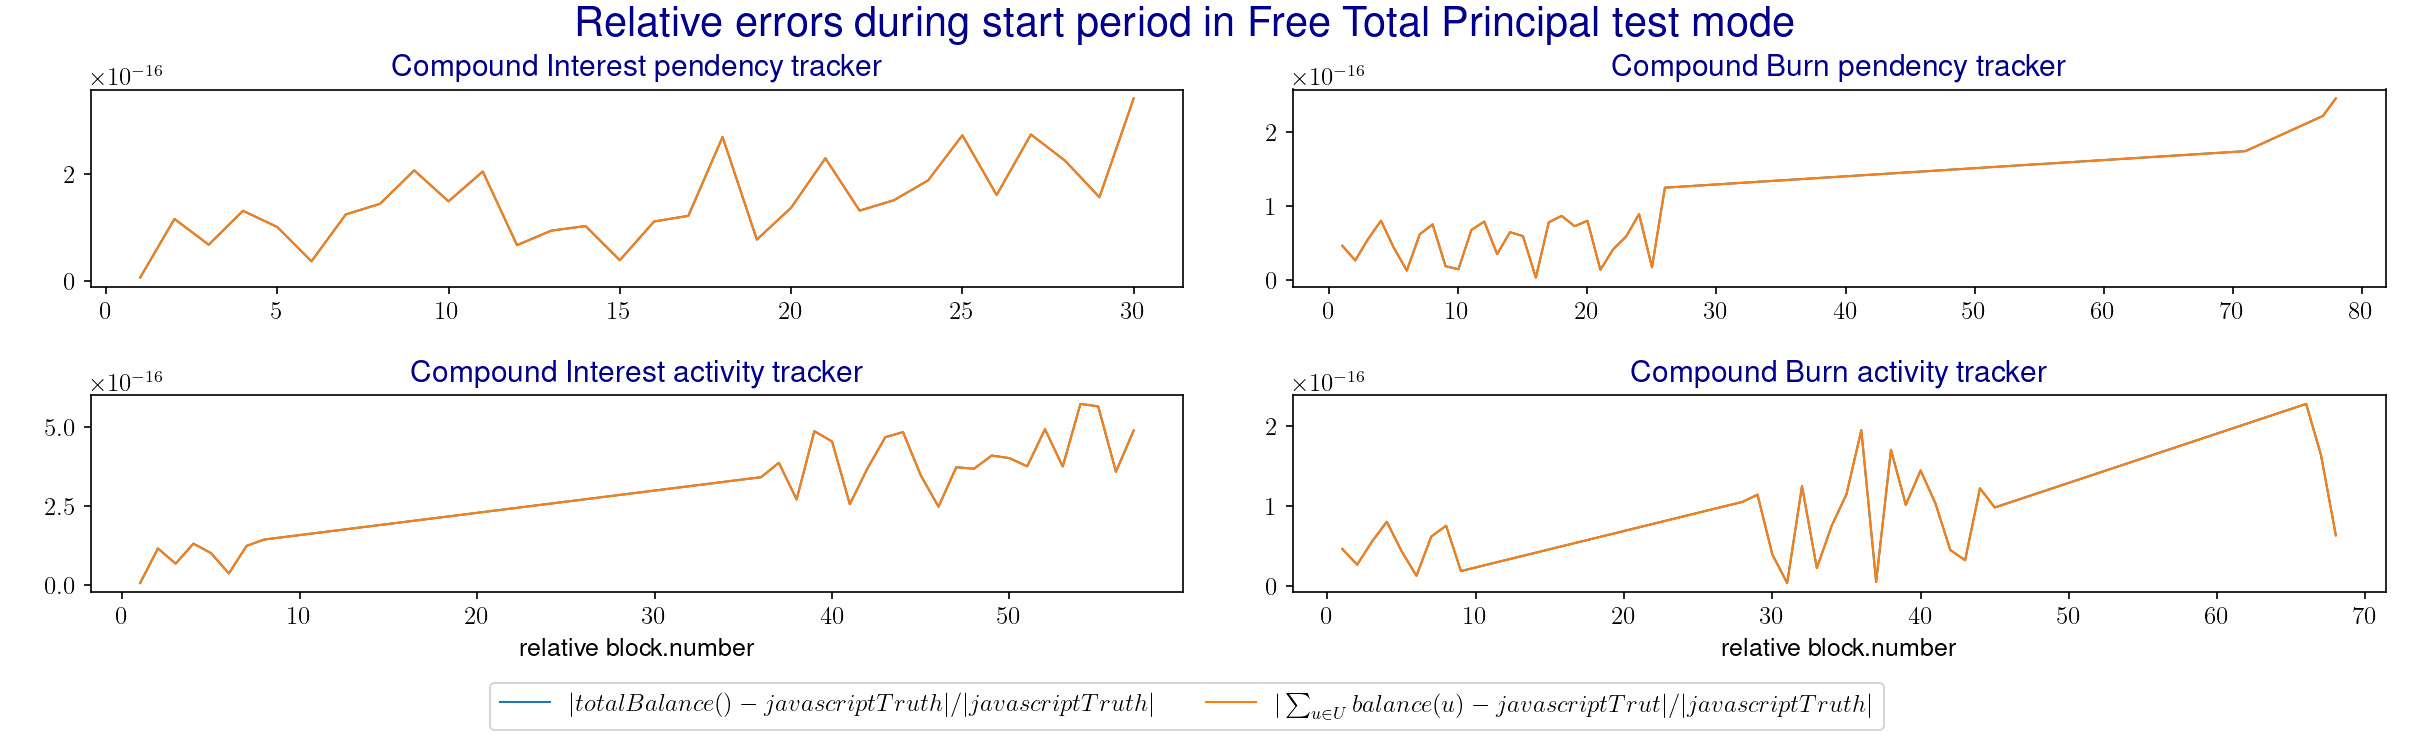
\includegraphics[width=5.3in]{images/6.3_free_com_relative_start.jpg}
  \caption{Relative Errors A and B, during the starting period, 
  for compound tasks in Free Total Principal test mode. 
  The two Relative Errors are not 
  distinguishable from each other on this small-resolution plot.
  }
  \label{fig:free_com_relative_start_case}
\end{figure}

\begin{figure}[H]
  \centering
  % \fbox{\rule[-.5cm]{4cm}{4cm} \rule[-.5cm]{4cm}{0cm}}
  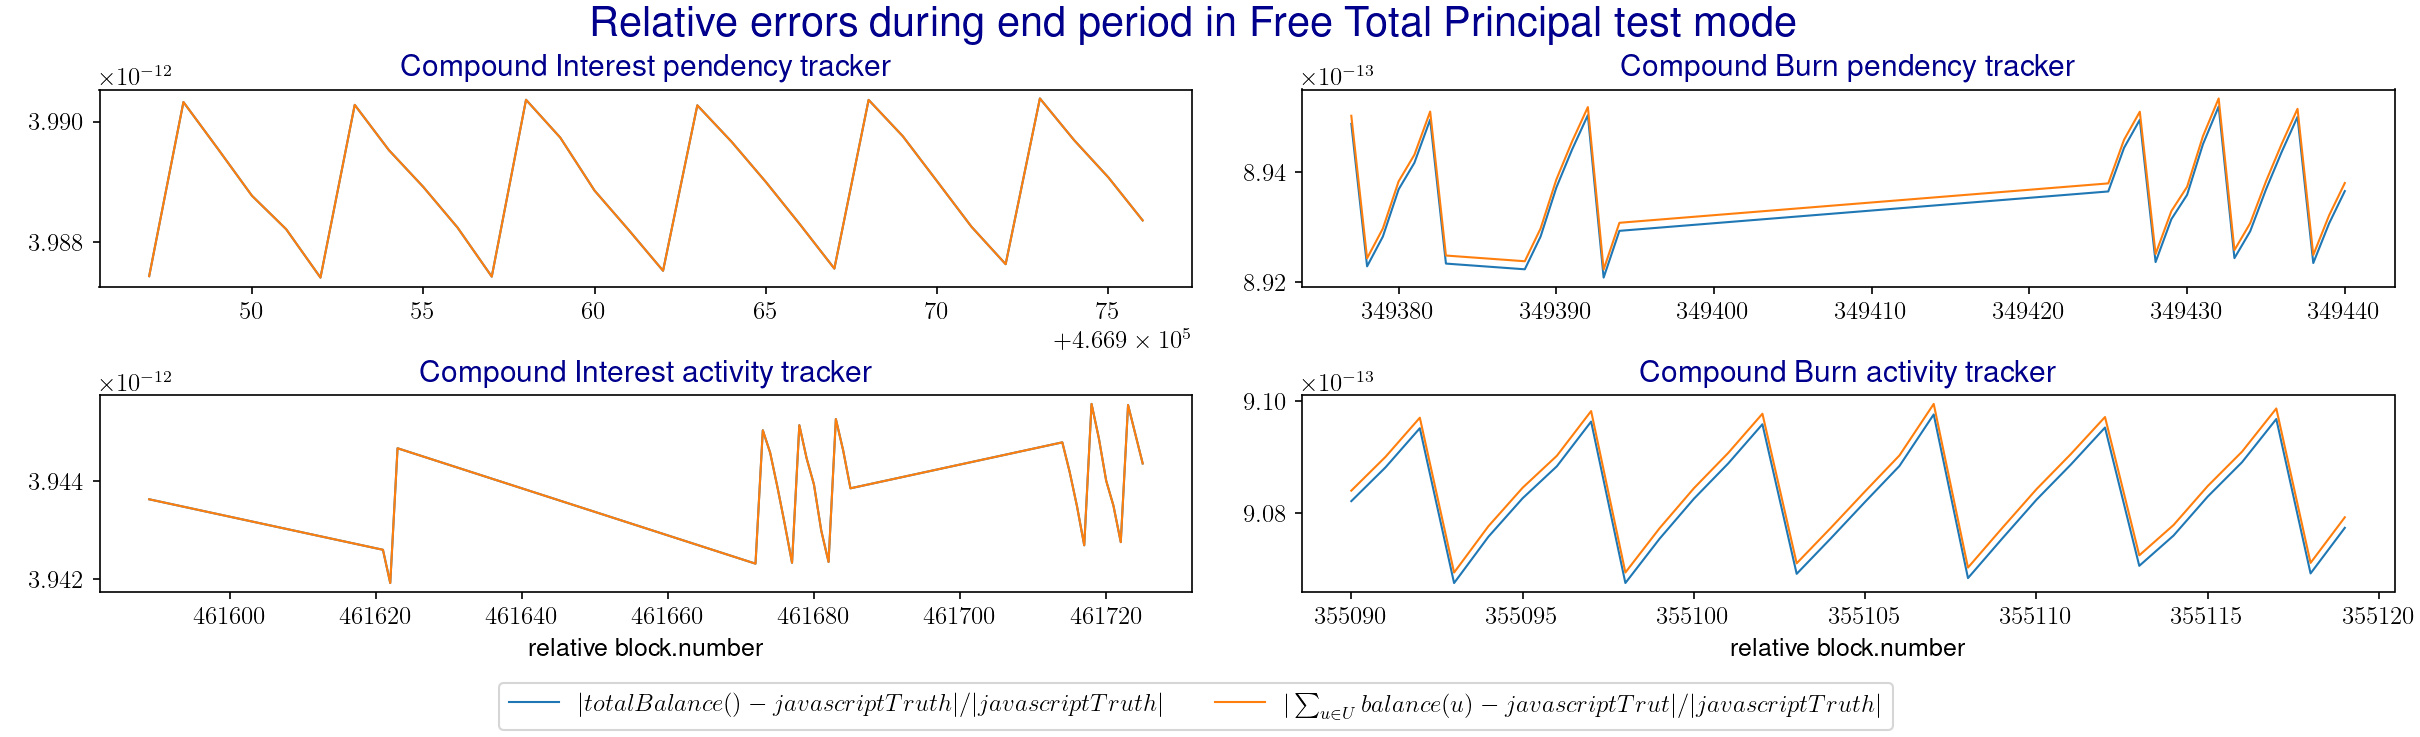
\includegraphics[width=5.3in]{images/6.3_free_com_relative_end.jpg}
  \caption{Relative Errors A and B, after a long run, 
  for compound tasks in Free Total Principal test mode. 
  The two Relative Errors are barely 
  distinguishable from each other for burn tasks. 
  }
  \label{fig:free_4_pillars}
\end{figure}

\subsection{Test case: Simple Tasks in Fixed Total Principal mode}

\begin{figure}[H]
  \centering
  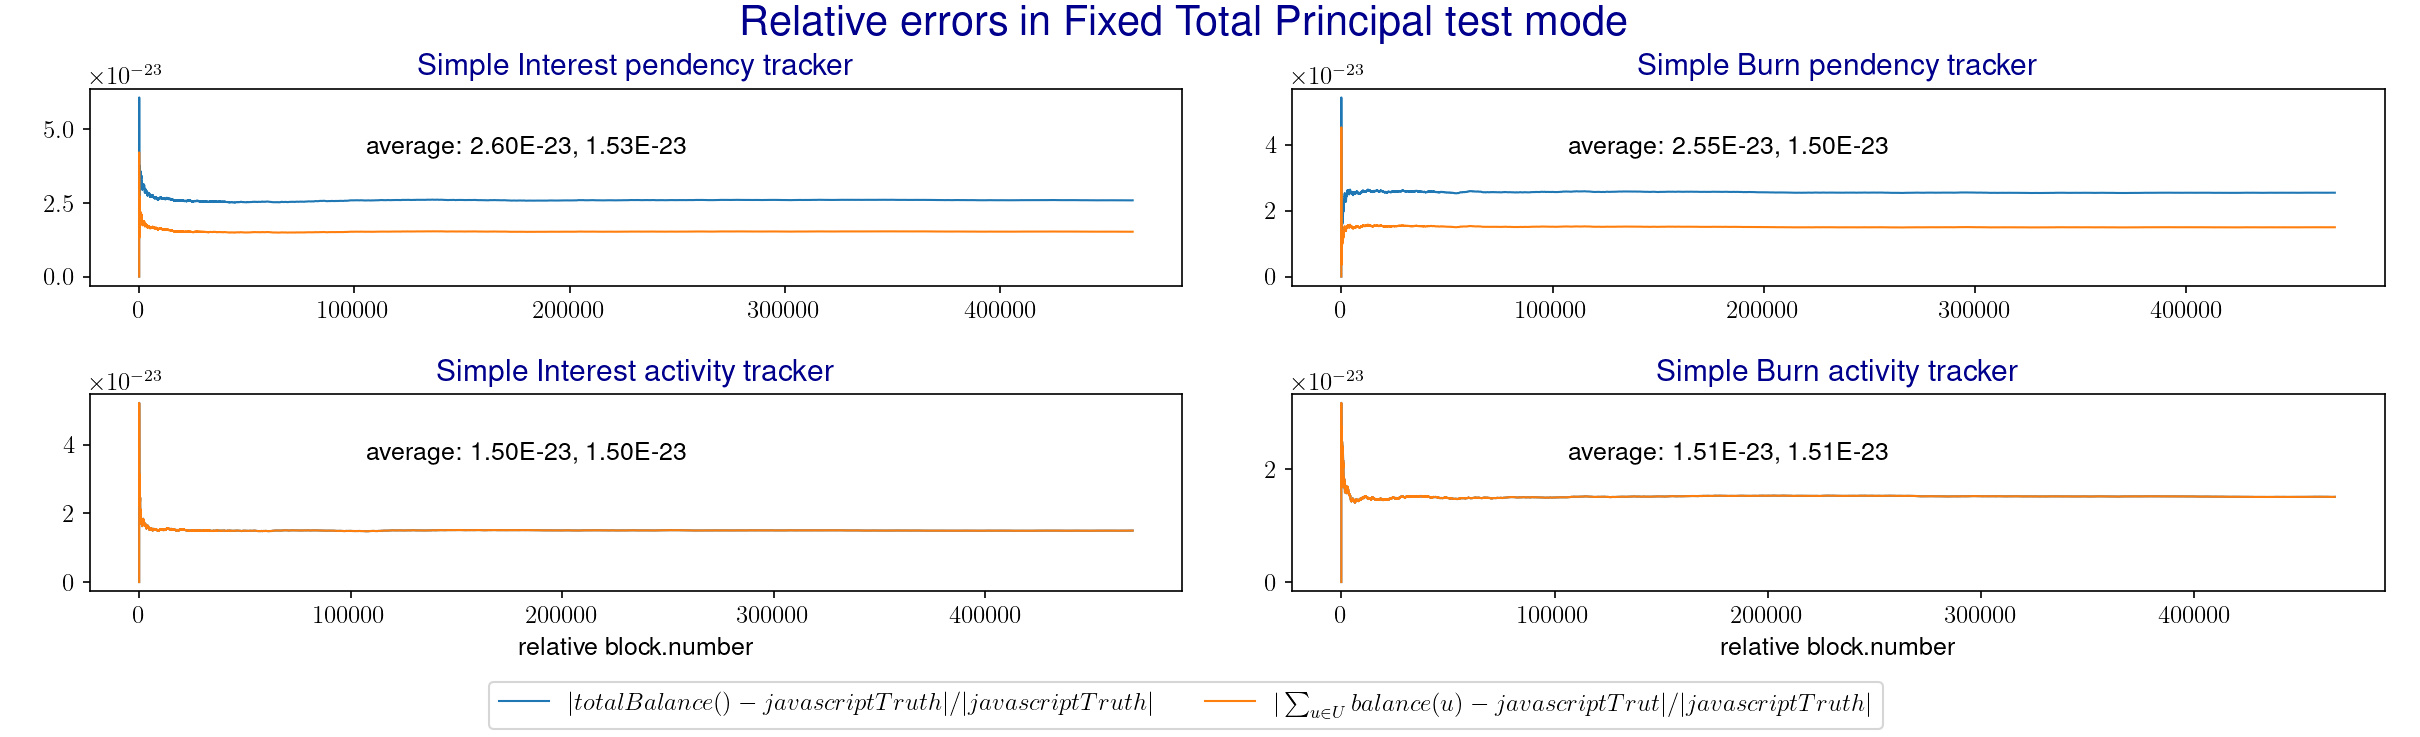
\includegraphics[width=5.3in]{images/6.3_fixed_sim_relative.jpg}
  \caption{Relative Errors A and B for simple tasks 
  in Fixed Total Principal test mode.
  }
  \label{fig:fixed_sim_relative_case}
\end{figure}

\begin{figure}[H]
  \centering
  % \fbox{\rule[-.5cm]{4cm}{4cm} \rule[-.5cm]{4cm}{0cm}}
  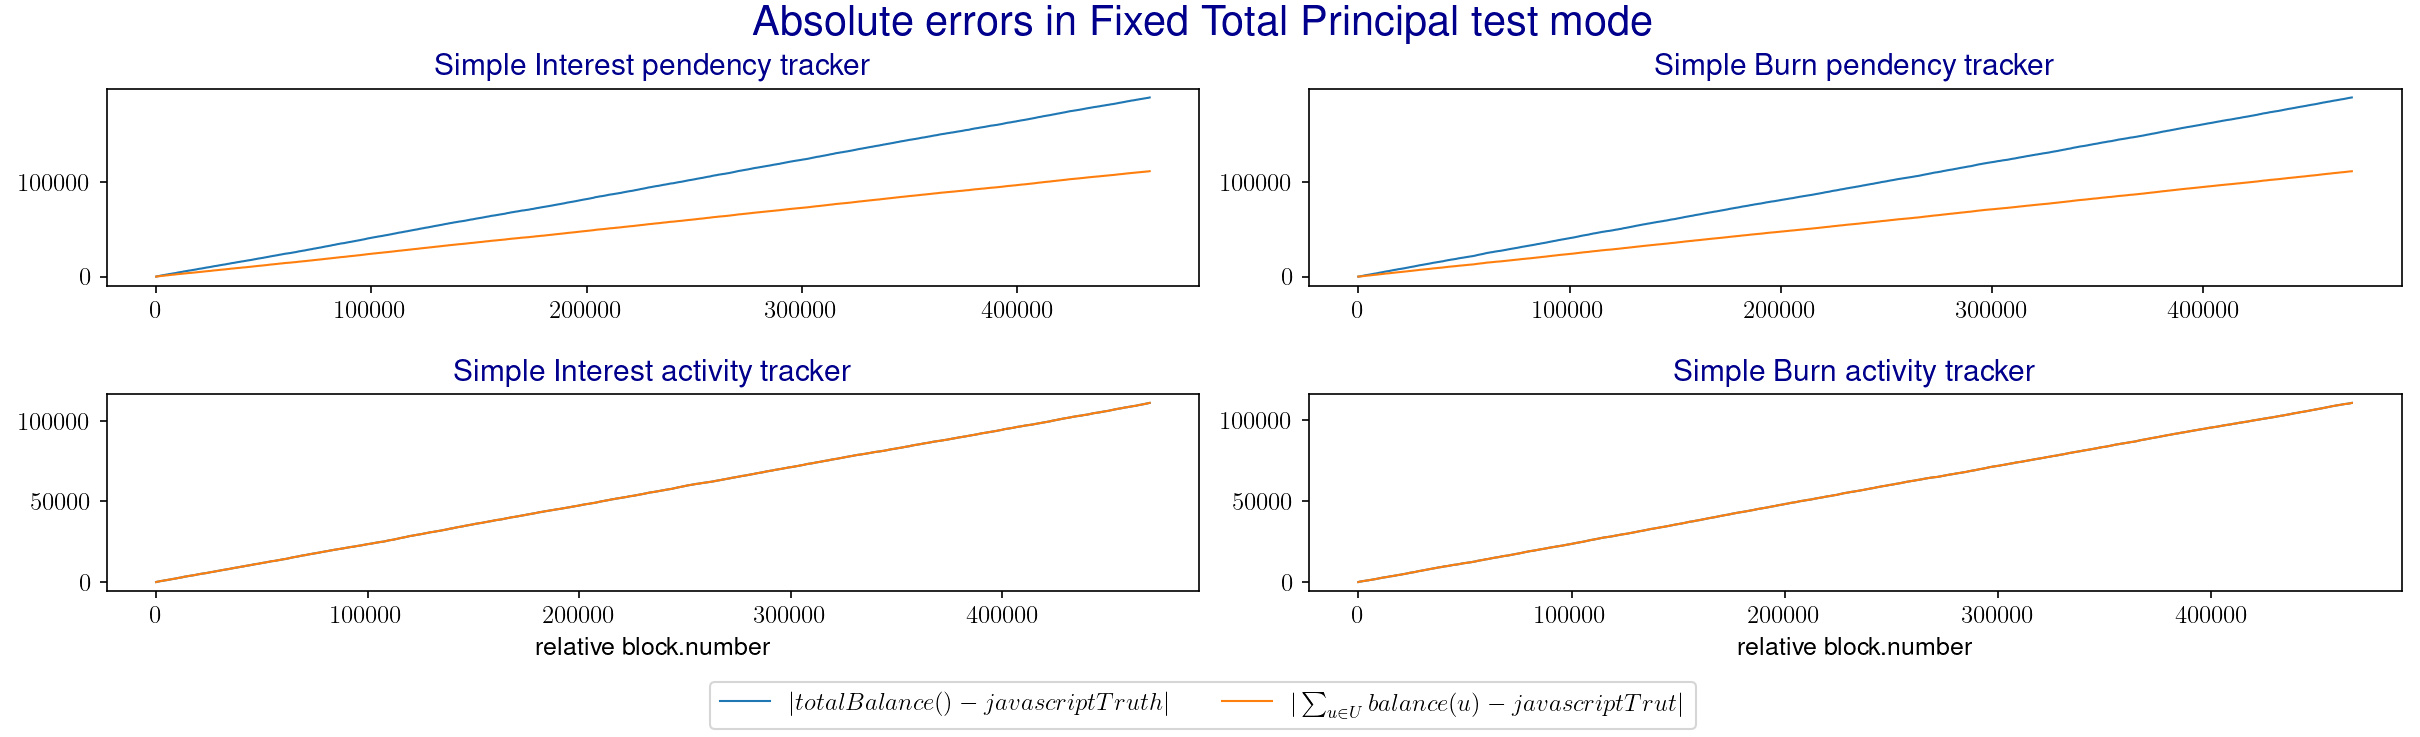
\includegraphics[width=5.3in]{images/6.3_fixed_sim_absolute.jpg}
  \caption{Absolute Consistency Errors for simple tasks 
  in Fixed Total Principal test mode. Activity tracker algorithms 
  show little, if not no, absolute errors.
  }
  \label{fig:fixed_sim_absolute_case}
\end{figure}

\begin{figure}[H]
  \centering
  % \fbox{\rule[-.5cm]{4cm}{4cm} \rule[-.5cm]{4cm}{0cm}}
  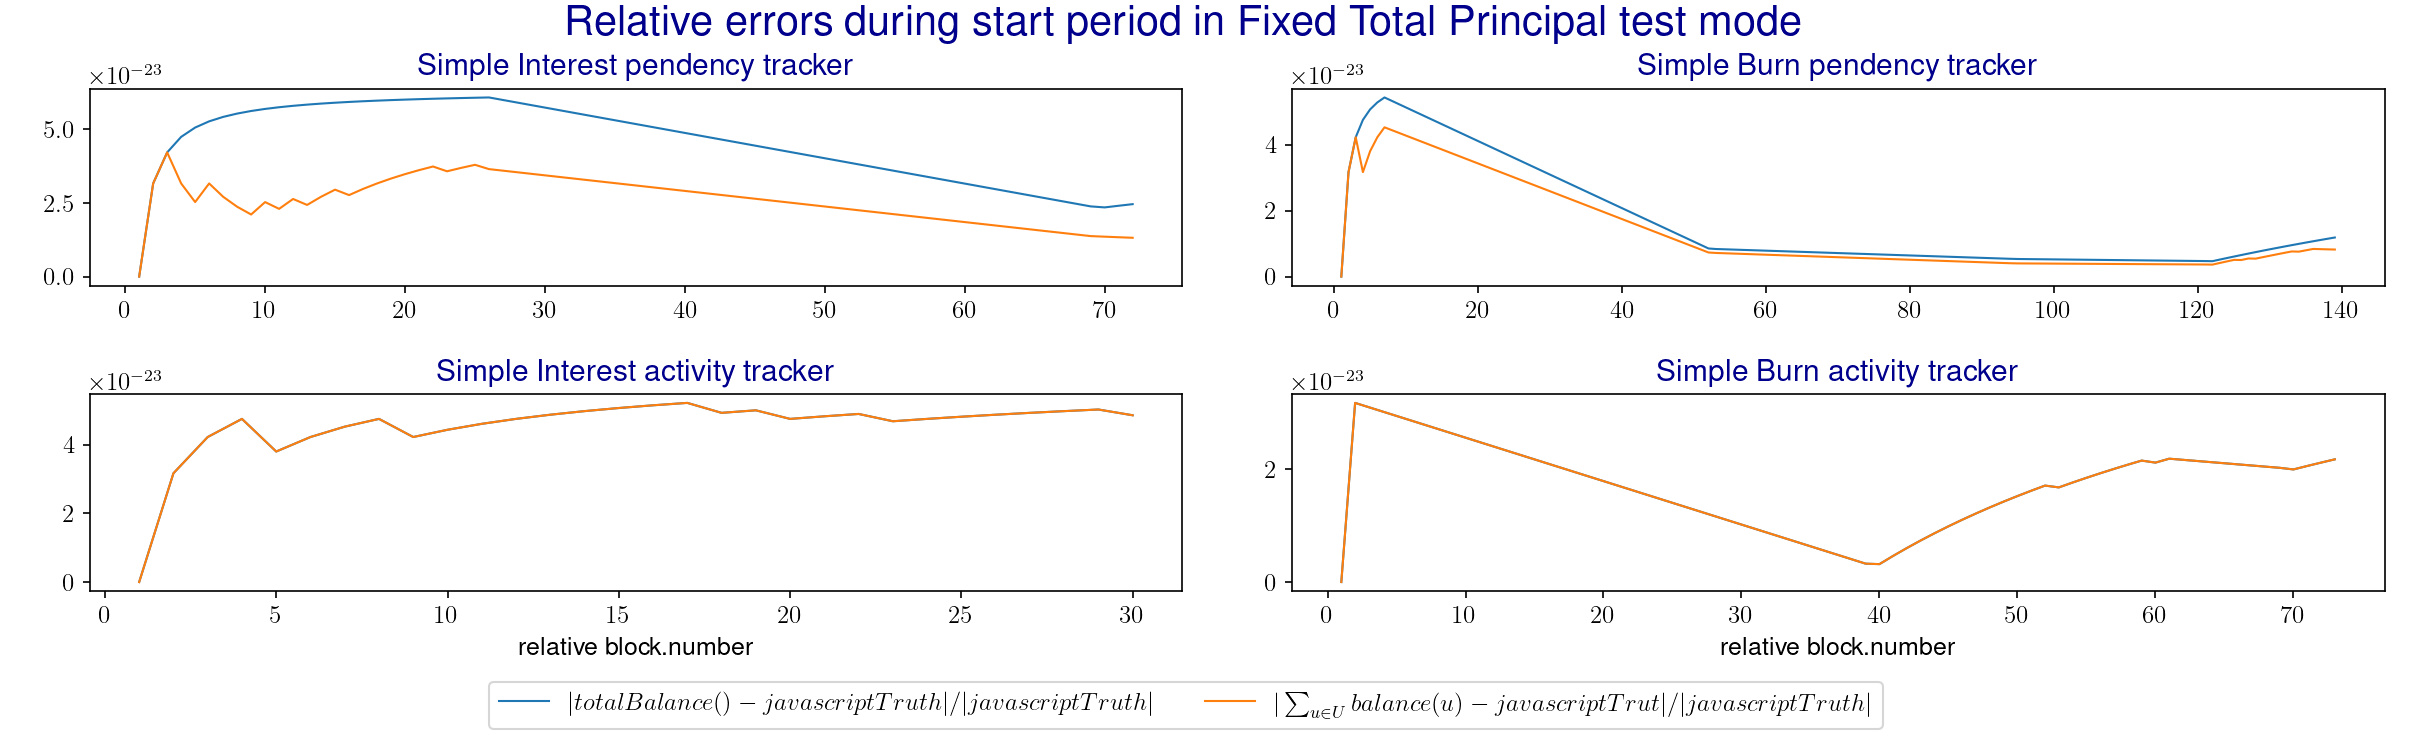
\includegraphics[width=5.3in]{images/6.3_fixed_sim_relative_start.jpg}
  \caption{Relative Errors A and B, during the starting period, for simple tasks 
  in Fixed Total Principal test mode.
  }
  \label{fig:fixed_sim_relative_start_case}
\end{figure}

\subsection{Test case: Compound Tasks in Fixed Total Principal mode}

\begin{figure}[H]
  \centering
  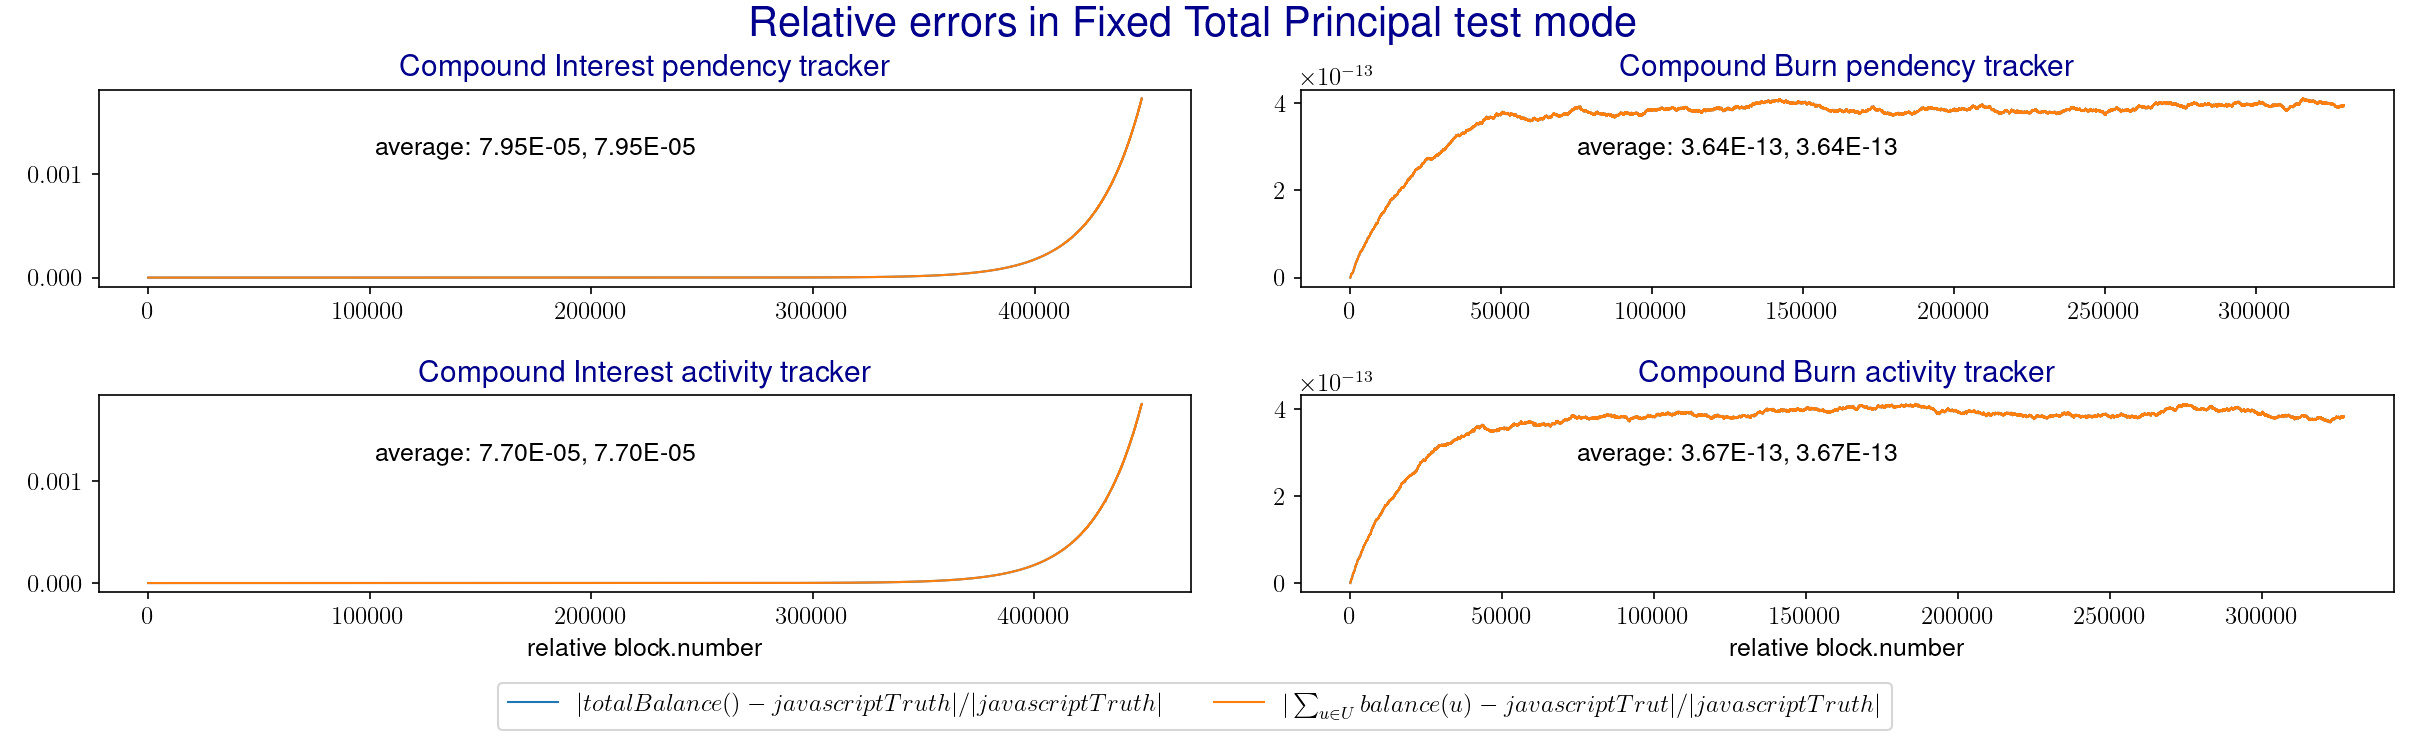
\includegraphics[width=5.3in]{images/6.3_fixed_com_relative.jpg}
  \caption{Relative Errors A and B for compound tasks 
  in Fixed Total Principal test mode. While Relative Errors are 
  not growing and lower than $10^{-12}$ in burn tasks, they are diverging  
  and as high as $0.002$, after a 128-year-long simulated run. 
  }
  \label{fig:fixed_com_relative_case}
\end{figure}

We guess the errors diverge, in the above chart, 
if the exponent is more than 1, as in 
interest tasks, where the exponent is $1+rate$; and converge if the 
exponent is less than 1, as in burn tasks, where the exponent is $1-rate$.
The interest rate $rate$ in this test scenario is $0.000474$, which is 
equivalent to about $1 \%$ every 21 days.

\begin{figure}[H]
  \centering
  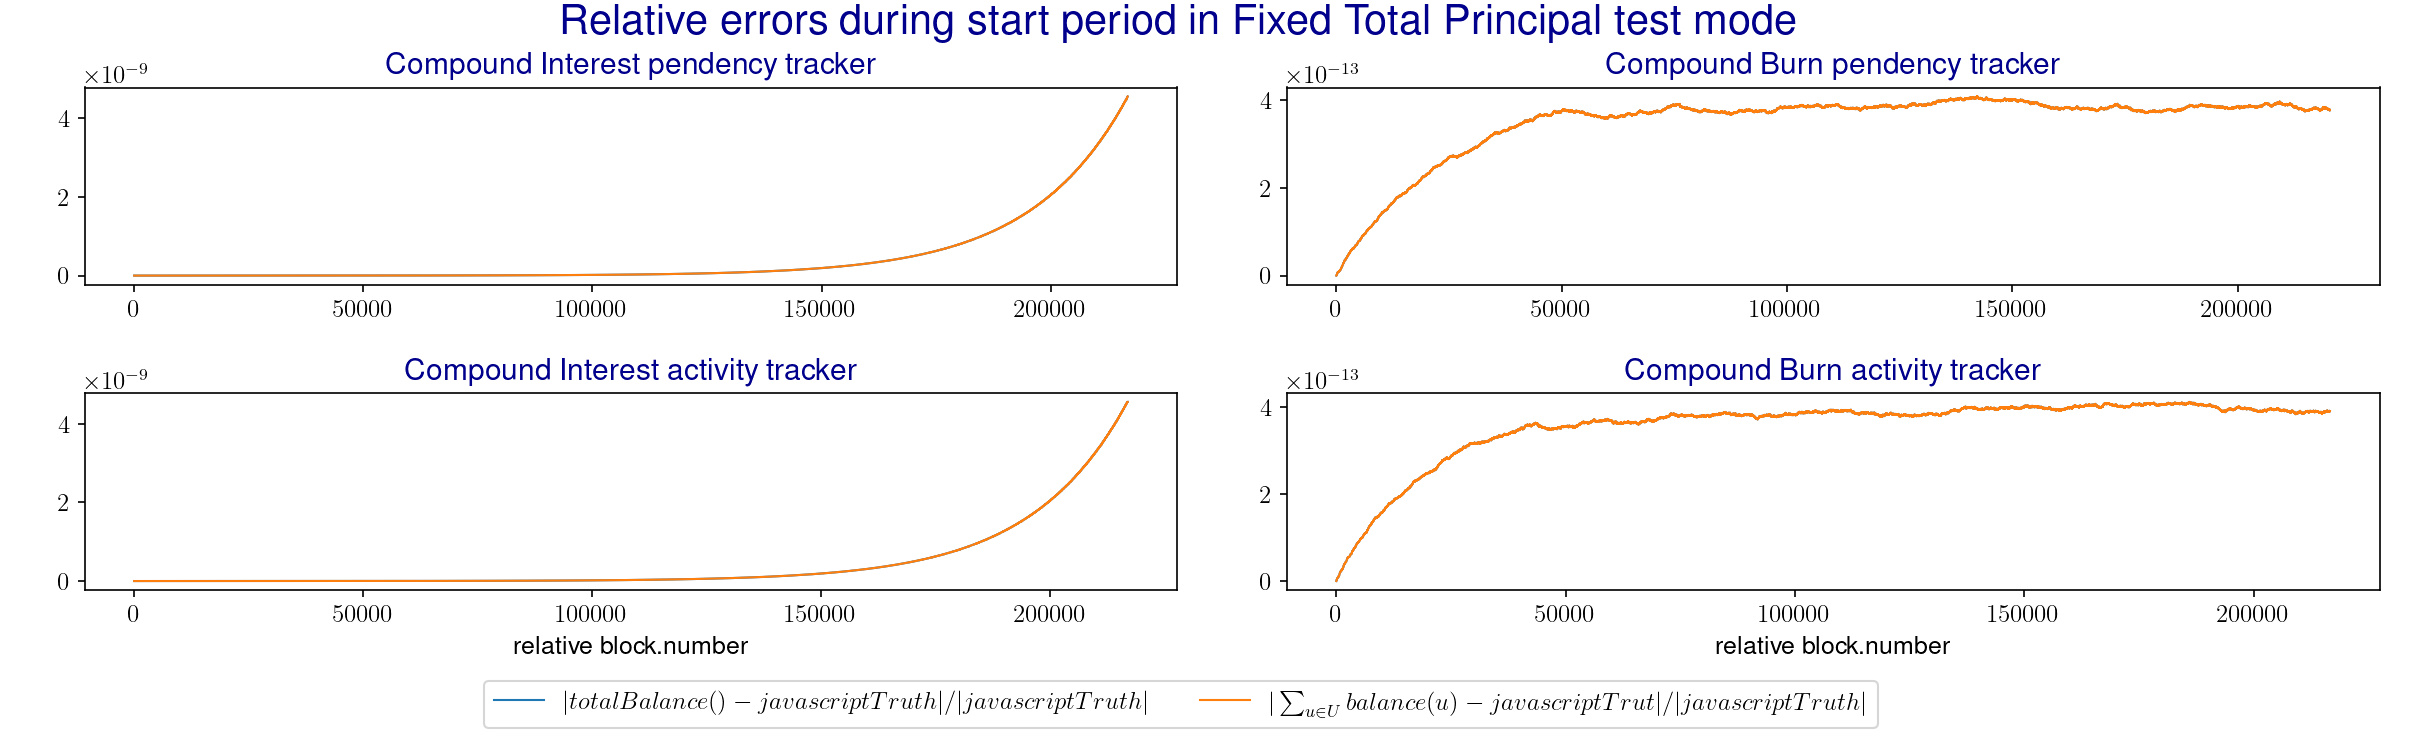
\includegraphics[width=5.3in]{images/6.3_fixed_com_relative_mid.jpg}
  \caption{Relative Errors A and B for compound tasks 
  in Fixed Total Principal test mode.
  }
  \label{fig:fixed_com_relative_case_mid}
\end{figure}

Unlike in Figure~\ref{fig:fixed_com_relative_case}, where the time span 
is 128 years,
the above chart spans only 60 simulated years.
The Relative Errors A and B for interest tasks 
are lower than $10^{-8}$, which is within the safe level.

\begin{figure}[H]
  \centering
  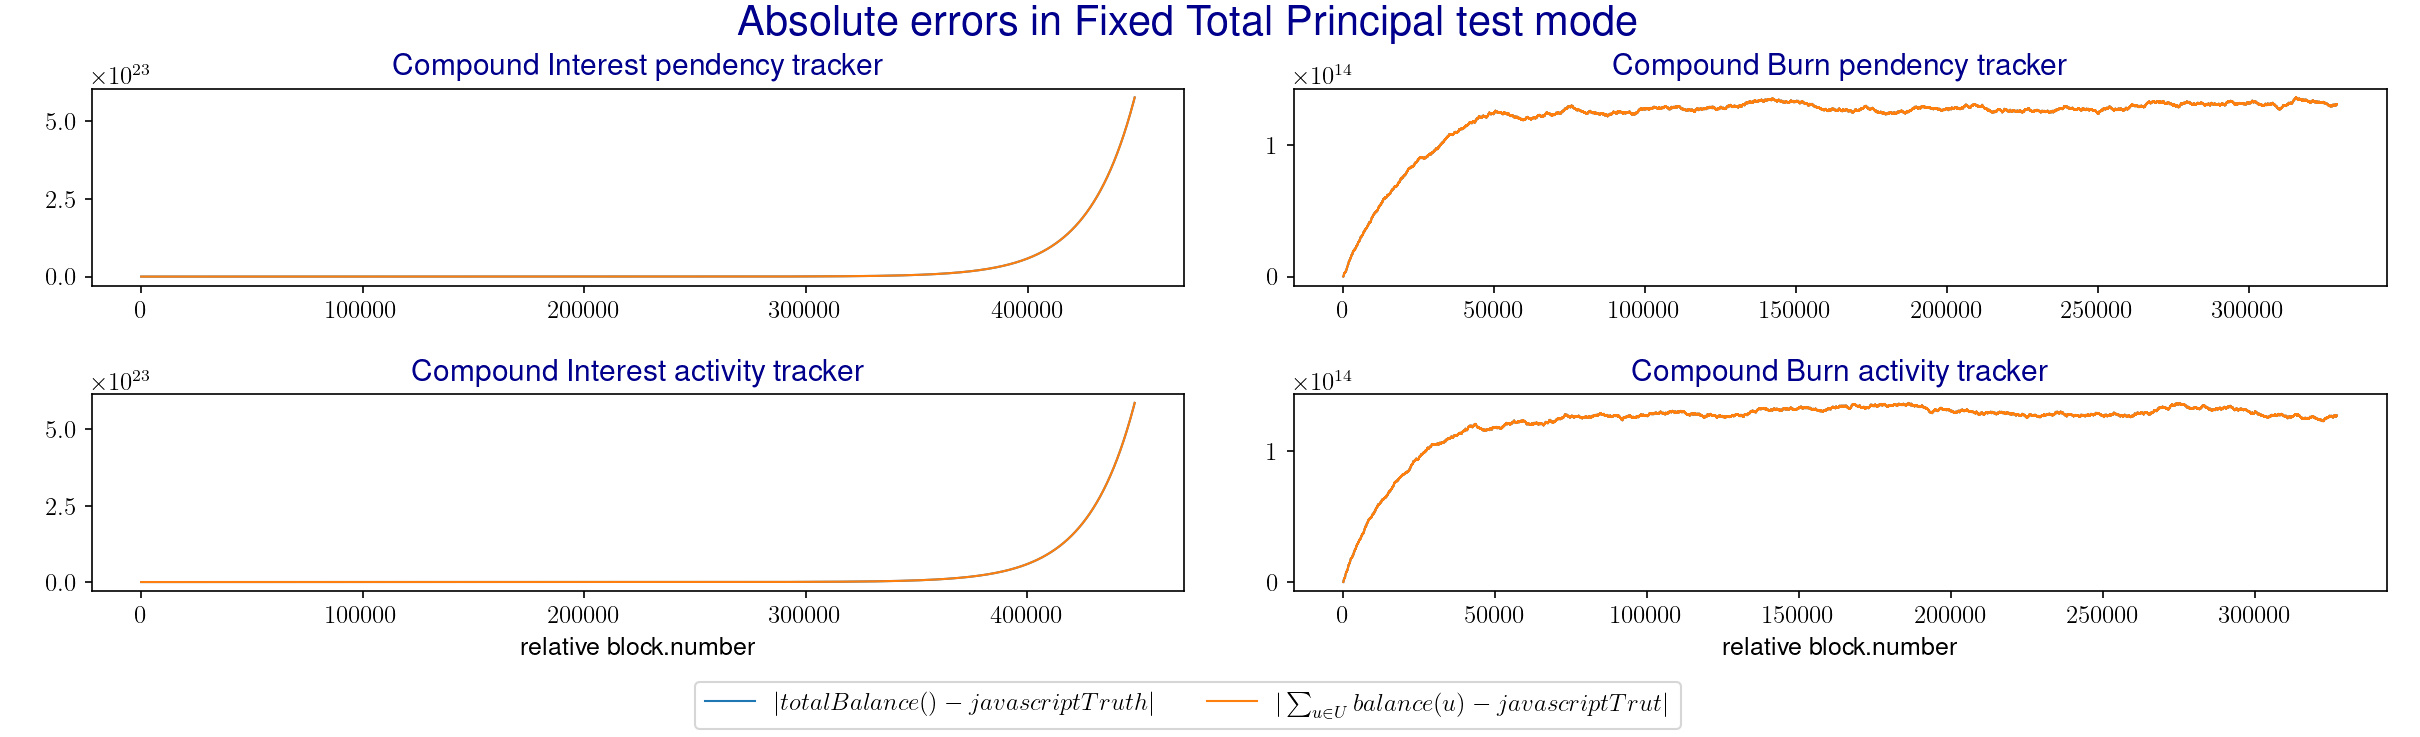
\includegraphics[width=5.3in]{images/6.3_fixed_com_absolute.jpg}
  \caption{Absolute Consistency Errors for compound tasks 
  in Fixed Total Principal test mode.
  }
  \label{fig:fixed_com_absolute_case}
\end{figure}

We guess, on the left of the above chart, 
that the exponentiation 
errors are time-exponential, which are successively accumulated 
to form new time-exponential errors.

\begin{figure}[H]
  \centering
  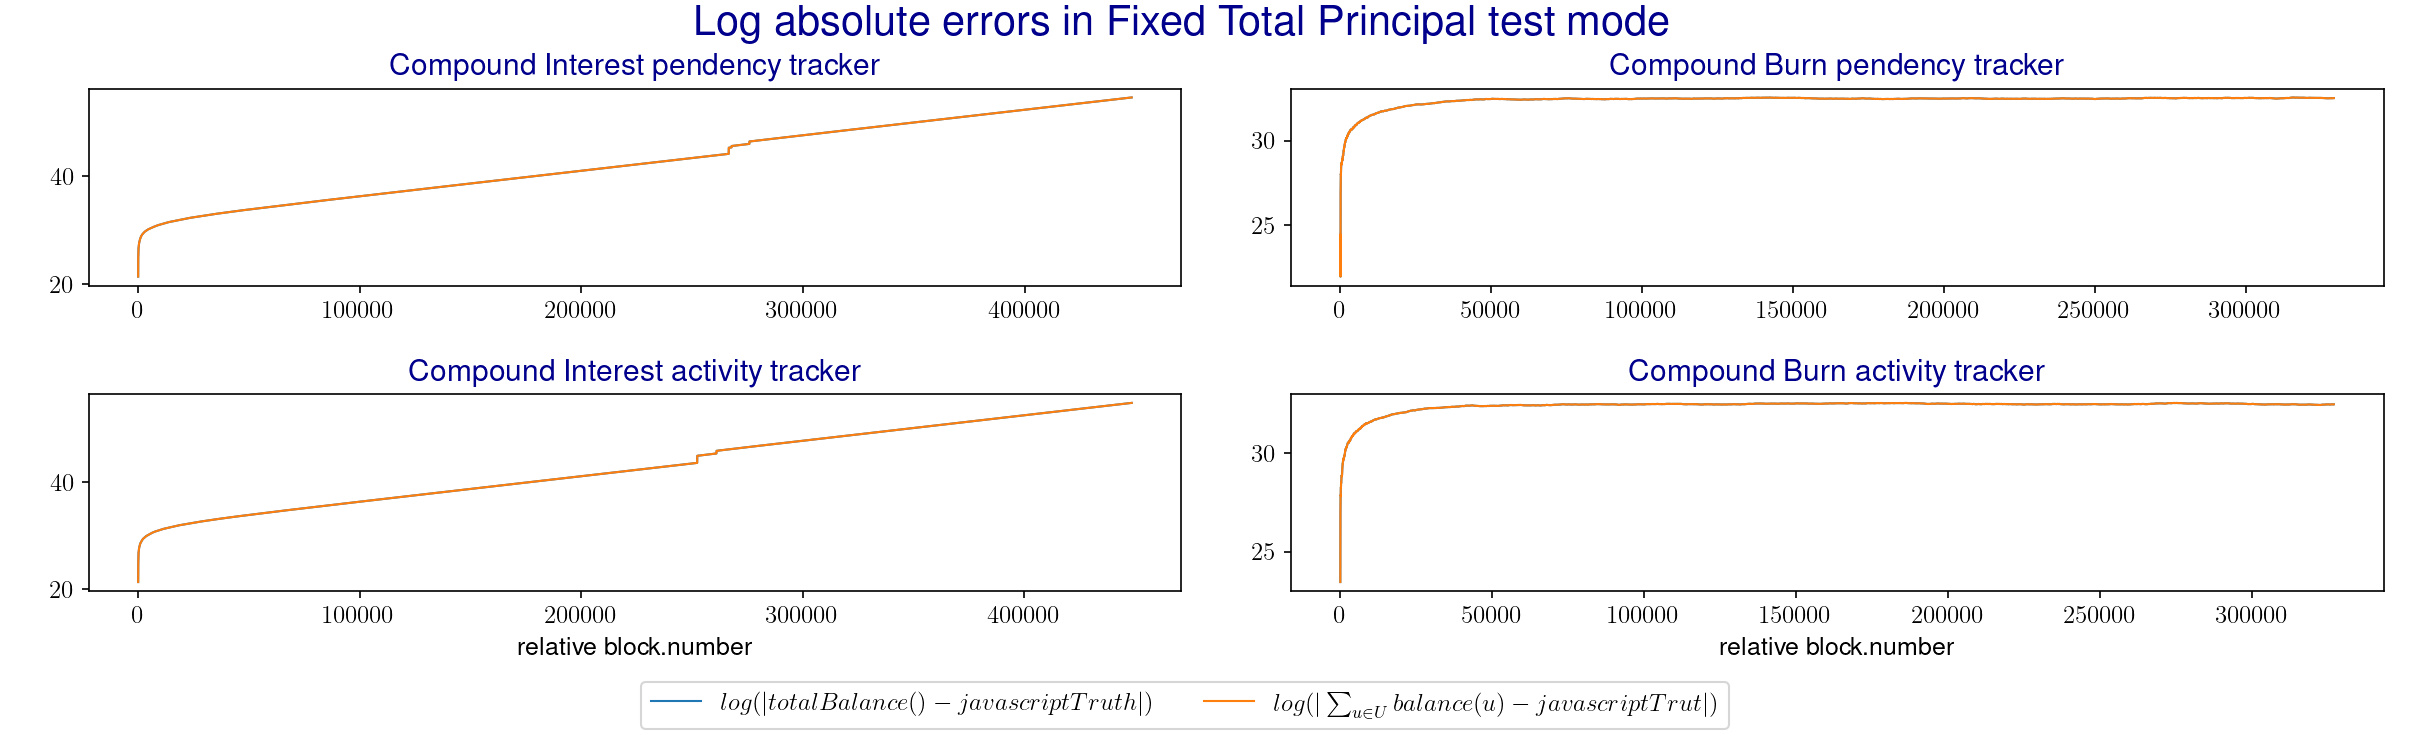
\includegraphics[width=5.3in]{images/6.3_fixed_com_absolute_log.jpg}
  \caption{Log Absolute Consistency Errors for compound tasks 
  in Fixed Total Principal test mode. The straight log lines on the left of the 
  chart confirms that the exponentiation errors are time-exponential.
  }
  \label{fig:fixed_com_absolute_log_case}
\end{figure}

\section{Conclusion}
\label{sec:Conclusion}

We proposed, proved, and demonstrated algorithms that solve Simple Interest,
Simple Burn, Compound Interest, and Compound Burn reward distribution tasks. 
The algorithms can distribute rewards to an unknown number of users, 
adhering to the computational quota  
if there are no computer numerical errors.
Although computer numerical errors are individually trivial, 
they collectively create a large deviation because the algorithms 
inherently and constantly accumulate amount figures that have numerical errors.
Table~\ref{tbl:RelativeErrors} shows Relative Errors A and B in 
various types of task and test modes.

Exponentiation errors turn out to be small if users' rewards are collected frequently, 
but grow harmful if they are accumulated over 
an extensively long period or a large number of transactions.
Division errors are also proved 
to be small enough to ignore compared to the huge magnitude of asset amount figures, 
unless we have an extremely large number of transactions.

\begin{table}[H]
  % \begin{center}
    \begin{spacing}{1.8}\centering
      \fontsize{8pt}{8pt}\selectfont
      \begin{tabular} {|m{2.4cm}|m{5.6cm}|m{6cm}|}
      \hline
      {\textbf{Task type}} & {\textbf{Free Total Principal test mode}} & {\textbf{Fixed Total Principal test mode}} \\
      \hline
      {\textbf{Simple Interest}} & {Keeps around tiny values, below $10^{-22}$} & {Keeps around a value, below $10^{-22}$} \\[3mm]
      \hline
      {\textbf{Simple Burn}} & {Keeps around tiny values, below $10^{-22}$} & {Keeps around tiny values, below $10^{-22}$} \\[3mm]
      \hline
      {\textbf{Compound Interest}} & {\textit{Diverges} slowly linearly, $4 * 10^{-12}$ after 128 years } & {\textit{Diverges} slowly but \textit{exponentially}, \newline $2 * 10^{-2}$ after 128 years, $5 * 10^{-9}$ after 60 years } \\[3mm]
      \hline
      {\textbf{Compound Burn}} & {\textit{Diverges} slowly linearly, $10^{-12}$ after 128 years} & {Converges to a small value, below $10^{-12}$} \\[3mm]
      \hline
    \end{tabular}
    \end{spacing}
  % \end{center}
  \caption {Relative Errors A and B in our test scenario.
  }
  \label{tbl:RelativeErrors}
  \end{table}

We leave mitigating numerical errors to future work, because that 
will require a significant amount of extra time.

We introduced new concepts and notations that can be reused in 
rigorous reasoning 
of decentralized techniques. We compared verbal proof and symbolic proof of 
decentralized algorithms and demonstrated symbolic proof may be more thorough and effective.

\section*{Acknowledgments}
\label{Acknowledgments}

We are deeply indebted to 
Calum Roberts, Dong-Zhe Lian, and Xavier Mitchell-Diggens
for their professional reviews and proofreading,
and excellent expertise in Decentralized Applications and academic writing.
This endeavor would not have been possible without Zheng-Yu Cai, who 
provided continuing administrative support and heartfelt encouragement.
I, the $1^{st}$ author, would like to express my deepest gratitude to 
my Mom, Dad, siblings, and wife for their wholehearted support.

\nocite{*}
\printbibliography

\end{document}



